\documentclass[]{tesis-usach}
% Opciones: coguia, propuesta

\usepackage{eurosym} % Para utilizar el símbolo \euro
\usepackage{longtable} % for add multi-page tables

\begin{document}
\baselineskip 23pt
\frontmatter								% Utiliza numeración romana

% ### Cubierta de la tesis ###
\thispagestyle{empty}
\facultad{Ingeniería}
\departamento{Informática}
\grado{Ingeniero Civil en Informática}

\titulo{Desarrollo de un SDK para dar soporte a OpenGlove en dispositivos móviles}

\autor{Israel Gedeón Elías Matínez Montenegro}
\email{nombre.apellido@usach.cl}
\run{12.345.678-9}		% S\'olo necesario en propuesta
\telefono{22222222}		% S\'olo necesario en propuesta
\annoingreso{Año}

\fecha{Lunes}{25}{Julio}{2018}

\profesorguia{Profesor Roberto González-Ibañez}
\profesorcoguia{Profesor(a) Co-Gu\'ia}

\ciudad{Santiago}
\pais{Chile}

\makecubierta


% ### Páginas preliminares de la tesis ###
\pagestyle{fancy}
\renewcommand{\headrulewidth}{0pt}		% Hace que no aparezca la línea horizontal superior al principio de estas páginas
\fancyhead[L]{}
\fancyhead[C]{}
\fancyhead[R]{}

{\setstretch{1.0}						% Interlineado en las páginas preliminares
\makecopyright							% Si es propuesta no se mostrará

% ### Resumen de la tesis
\setcounter{page}{0} 
\resumenCastellano{
OpenGlove es un dispositivo diseñado en el Departamento de Ingeniería Informática por el grupo de investigación InTeracTion perteneciente a la Universidad de Santiago de Chile. El guante permite la retroalimentación vibrotáctil o \textit{haptic feedback} cuando se interactúa con objetos en ambientes de realidad virtual (VR), aumentada (AR) o mixta (MR). Esta retroalimentación es generada a través de la vibración de motores distribuidos en distintas partes del guante, distribución que depende de los requerimientos del usuario o la aplicación. El guante también sensores de flexibilidad para la captura del movimiento de los dedos y una unidad de medición inercial o IMU(Inertial Measurement Unit) para capturar la orientación de la mano.

%OpenGlove fue concebido para que pueda ser utilizado en conjunto con otros dispositivos, tales como Oculus Rift, Kinect y Leap Motion. OpenGlove actualmente soporta un servicio bluetooth en Windows para la conexión de dispositivos. El guante adicionalmente soporta el uso de sensores de flexibilidad  y una unidad de medición inercial o IMU (Inertial Measurement Unit).

Si bien es posible tener una inmersión en estos ambientes,  esta es parcial, dejando de lado el sentido del tacto. El estado actual de OpenGlove no permite el uso del mismo en comunidades de desarrollo de VR, AR y MR en entornos móviles como Android e iOS. Esto limita la portabilidad y desacople del sistema operativo Windows. Por ello lo que se propone es dar soporte a OpenGlove en dispositivos móviles enriqueciendo la interacción en los entornos ya mencionados.
%Como
Esto se realizó mediante el desarrollo de un SDK para dispositivos móviles, el cual permite la conexión por Bluetooth de varias instancias de OpenGlove, como también la  configuración de los mismos mediante la carga de perfiles utilizando una aplicación de configuración. Esta aplicación expone un servicio, el cual es utilizado mediante las APIs en Java y C\#. Se realizaron evaluaciones de rendimiento y pruebas de concepto utilizando el sistema propuesto.

% el qué, el cómo, para qué y por qué

%OpenGlove es un dispositivo que permite la retroalimentación vibrotáctil en ambientes de realidad virtual. Fue diseñado en la Universidad de Santiago de Chile, su diseño es flexible dado que no se limita a una ubicación en especial de los dispositivos vibrotáctiles. Los prototipos realizados utilizan motores que generan vibraciones cuando se interactúa  con objetos en un entorno virtual o de realidad aumentada. OpenGlove se ha pensado para que pueda ser utilizado en conjunto con otros dispositivos, como Oculus Rift, Kinect y Leap Motion. Por otra parte, los prototipos de OpenGlove utilizan motores configurables con diferentes niveles de potencia, lo que permite la respuesta vibrotáctil en distintas áreas de la mano, lo cual puede ser utilizado para representar la sensación de tocar objetos en entornos virtuales, como también, recibir retroalimentación que represente impacto, el cual sería útil en un juego de boxeo por ejemplo.   Actualmente, el proyecto OpenGlove considera una arquitectura que involucra el guante que utiliza una placa Arduino LilyPad, con el cual puede ser configurado y utilizado mediante el SDK y la API de bajo nivel. Luego en un nivel superior de la arquitectura, existe un servicio que utiliza SOAP y REST para exponer los servicios mediante bluetooth en Windows y hacer uso del guante, como también el configurar parámetros de los componentes del guante. Finalmente, las  APIs de alto nivel para lenguajes de programación como C\#, C++, Java, y JavaScript implementadas el 2016, permiten desacoplamiento y abstraen  la complejidad en el uso de instancias y configuración de OpenGlove. El estado actual de OpenGlove no permite el uso del mismo en comunidades de desarrollo de realidad virtual móvil en Android, limitando con ello la portabilidad y desacople del sistema operativo Windows. Por ello lo que se propone es dar soporte a OpenGlove en dispositivos móviles. Esto se realizará mediante el desarrollo de una aplicación nativa en Android, que permitirá levantar un servicio bluetooth para el uso de varias instancias de OpenGlove, como también la configuración de los guantes, mediante la carga de perfiles. También se desarrollará un SDK para facilitar los futuros desarrollos en dispositivos móviles. Se realizarán evaluaciones de rendimiento y pruebas de concepto utilizando el sistema propuesto.

\vspace*{0.5cm}
\KeywordsES{ Haptic Feedback; Virtual Reality (VR); Augmented Reality (AR); Mixed Reality (MR); OpenGlove; SDK; API}
}

%\newpage

%\resumenIngles{
%Contrary to popular belief, Lorem Ipsum is not simply random text. It has roots in a piece of classical Latin literature from 45 BC, making it over 2000 years old. Richard McClintock, a Latin professor at Hampden-Sydney College in Virginia, looked up one of the more obscure Latin words, consectetur, from a Lorem Ipsum passage, and going through the cites of the word in classical literature, discovered the undoubtable source. Lorem Ipsum comes from sections 1.10.32 and 1.10.33 of "de Finibus Bonorum et Malorum" (The Extremes of Good and Evil) by Cicero, written in 45 BC. This book is a treatise on the theory of ethics, very popular during the Renaissance. The first line of Lorem Ipsum, "Lorem ipsum dolor sit amet..", comes from a line in section 1.10.32.

%The standard chunk of Lorem Ipsum used since the 1500s is reproduced below for those interested. Sections 1.10.32 and 1.10.33 from "de Finibus Bonorum et Malorum" by Cicero are also reproduced in their exact original form, accompanied by English versions from the 1914 translation by H. Rackham.

%\vspace*{0.5cm}
%\KeywordsEN{Key; words}
%}


% ### Dedicatoria y agredecimientos de la tesis ###
\dedicatoria{
Dedicado a...
}
		% En caso de no querer agregarlos, comente esta línea
\begin{agradecimiento}
Agradezco a
\end{agradecimiento}

% ### Índices ###
\tableofcontents							%% Tabla de contenido

\listoftables							%% Indice de tablas
\listoffigures							%% Indice de figuras
%\listofalgorithms						%% Indice de algoritmos (Optativo: En caso de poseer algoritmos)
\AtBeginEnvironment{algorithmic}{\setstretch{1.5}} % Interlineado de los algoritmos
} % end \setstretch{1.0}

% ### Cuerpo de la tesis ###
\mainmatter								% Reinicia el contador de páginas para partir de 1 y usando números arábicos.

% ### Capítulos de la tesis ###

%\newpage
\chapter{Introducción}
%%%%%%%%%%%%%%%%%%%%%%%%%%%%%%%%%%%%%%%%%%
% revisado = false
%%%%%%%%%%%%%%%%%%%%%%%%%%%%%%%%%%%%%%%%%%
%This is the introduction chapter that includes the previus seminary document.

	\section{Antecedentes y motivación}
%) Motivación: Esta sección explica el contexto y síntomas de un problema, así como las razones que justificarían resolverlo para alcanzar una situación deseada. Para esto, se describe una situación actual, normalmente indeseable, con datos o hechos relevantes, se identifica a quienes le ocurre, cuando les ocurre, como les ocurre, donde, etc., se identifican los principales síntomas indeseables de la situación. También se explican las consecuencias que tendría en las personas o en la comunidad si la situación actual se mantiene o se la deja evolucionar en forma natural. Normalmente las consecuencias son expresadas en alguna forma de pérdida continua o creciente: humana, material, económica, energética, oportunidades, eficiencia, etc. Se apoya sobre evidencia o referencias apropiadas respaldando las afirmaciones fuertes. Se argumenta sobre la importancia que tiene desarrollar una solución al problema y su impacto, o las consecuencias más relevantes que una solución tendría en las personas, en las empresas, o en alguna disciplina de conocimiento. Se describen finalmente los aspectos más relevantes de una situación deseada.

%Estilo OREO
%\textcolor{red}{AGREGAR OREO}
El tamaño del mercado de la realidad virtual (VR) \footnote{\textbf{Virtual Reality (VR):}  ``La realidad virtual (VR) proporciona un entorno 3D generado por computadora que rodea al usuario y responde a las acciones de esa persona de forma natural ..." \cite{gartner-group-VR}.}  y realidad aumentada (AR)\footnote{\textbf{Augmented Reality (AR):} ``es el uso de información en tiempo real en forma de texto, gráficos, audio y otras mejoras virtuales integradas con objetos del mundo real ... "" \citep{gartner-group-AR}} registra 6.1 billones de dólares para el año 2016 y se estima que para el 2017 ascienda a 11.4 billones \citep{statista-VR-AR}.  En este contexto también aparece la denominada realidad mixta (MR) \footnote{\textbf{Mixed reality (MR):} ``es el resultado de mezclar el mundo físico con el mundo digital,  incluyendo la interacción con objetos virtuales representados en el real ..." \citep{microsoft-MR}.} la cual es un punto intermedio entre VR y AR.  Actualmente es bastante popular el  uso de VR, AR y MR en dispositivos móviles, pero estos carecen del soporte de otros sentidos como lo es el tacto lo cual genera una disrupción cuando se interactúa con los objetos virtuales. En este contexto se puede presenta una brecha cuando se desea incluir retroalimentación vibrotáctil o el denominado \textit{haptic feedback}\footnote{\textbf{Haptic Feedback:} Haptics es una tecnología táctil o de retroalimentación de fuerza que aprovecha el sentido del tacto de una persona al aplicar vibraciones y / o movimiento a la punta del dedo del usuario ..." \citep{gartner-group-haptics}} a aplicaciones en los entornos ya mencionados. Adicionalmente se incluye la captura de movimiento, para su representación en  los ambientes ya mencionados.

%Para los años 2020 y 2021 las estimaciones esperan un tamaño de mercado de 143.3 billones de dólares y 215 billones de dólares 

En primer lugar, el tamaño del mercado entre el 2017 y 2020 para VR y AR espera más de un 1200\% de aumento en sumas de billones de dólares. Esto es una interesante oportunidad de negocio, como también el aprovechar las distintas comunidades de desarrollo de VR, AR y MR para masificar el uso de OpenGlove.

En segundo lugar, la disrupción que se genera cuando se interactúa con objetos virtuales y no se obtiene una respuesta similar a la experiencia real, crea un punto de quiebre entre lo real y lo virtual. Esto implica una inmersión parcial en los ambientes de VR, AR y MR.

En tercer lugar se tiene el alto costo asociados a la adquisición de los guantes. Es posible constatar precios de guantes que van desde los 300\euro \space hasta los 1300\euro \space y licencias desde los 2500\euro \space hasta los 13300\euro . Esto se traduce en costos más altos de desarrollo como también para los usuarios finales. Además genera un mercado con un alcance más limitado.

En base a los argumentos desarrollados, se evidencia una brecha en la inclusión de Haptic Feedback  y la captura de movimiento de las manos en proyectos de VR, AR y MR en dispositivos móviles, la cual actualmente no es cubierta de manera global.

El estado actual de OpenGlove no permite el uso del mismo en comunidades de desarrollo de VR, AR y MR en entornos móviles como Android e iOS. Esto limita la portabilidad y desacople del sistema operativo Windows, reduciendo el alcance que puede tener en las ya mencionadas comunidades de desarrollo.

%END OREO
%END MOTIVACION
    \section{Descripción del problema}
\label{seccion:descripcion-problema}
%%%%%%%%%%%%%%%%%%%%%%%%%%%%%%%%%%%%%%%%%%
% revisado = false
% actualizar diagrama de arquitectura con lo desarrollado por Rodrigo Cerda
%%%%%%%%%%%%%%%%%%%%%%%%%%%%%%%%%%%%%%%%%%

  %) Enunciado del problema: Aquí se define el problema a resolver, sin plantear una solución a priori. Incluir datos, precondiciones o antecedentes que sean necesarios para precisar el problema. Se sugiere plantearlo como una pregunta que desafíe al solucionador a buscar una forma de eliminar o reducir la tensión entre la situación actual indeseable y la situación deseada. Este enunciado debe ser consistente con el propósito de la solución.
  Actualmente el proyecto OpenGlove posee la  arquitectura que se aprecia en la Figura \ref{fig:arquitectura-open-glove}. El guante posee motores distribuidos en distintos lugares de la mano, los cuales pueden ser activados y desactivados según se requiera mediante APIs \citep{tesis-monsalve-rodrigo}, también se tienen sensores de flexibilidad y la captura de movimientos de la mano \citep{tesis-cerda-rodrigo} . Existe un servicio que utiliza SOAP y REST para exponer los servicios mediante Bluetooth en Windows. Luego las  APIs de alto nivel \citep{tesis-meneses-sebastian} para lenguajes de programación como C\#, C++, Java, y JavaScript , permiten la abstracción de  la complejidad en el uso de instancias y configuración de OpenGlove. El estado actual de OpenGlove no permite el uso del mismo en comunidades de desarrollo de realidad virtual móvil en Android VR\footnote{Comunidad Android: \url{https://developers.google.com/vr/android/}}, ni iOS \footnote{Comunidad iOS: \url{https//developers.google.com/vr/ios/}} sin depender del sistema que permite la configuración y la ejecución del servicio en Windows. Lo cual dificulta la integración de OpenGlove para soluciones en dispositivos móviles y la independencia de servicios alojados en otro sistema operativo,  para poder desarrollar aplicaciones de VR, AR o MR para dispositivos móviles.
  
El problema se puede resumir en la siguiente pregunta  ¿Cómo facilitar a la comunidad de desarrolladores de VR/AR/MR a integrar OpenGlove en entornos móviles y realizar una fácil configuración para los dispositivos?.
  
  \begin{figure}[H]
  \begin{center} 
   	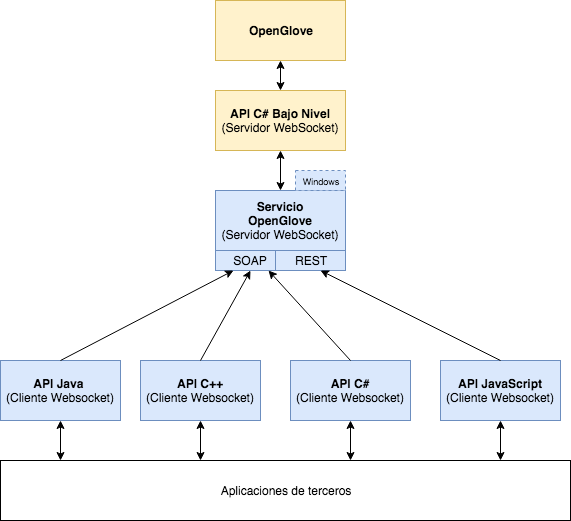
\includegraphics[width=0.5\textwidth]{images/chapter01/Legacy-OpenGlove-Architecture-02.png} 
    \caption[Arquitectura OpenGlove]{Arquitectura OpenGlove \\Fuente: Elaboración propia (2018)}
    \label{fig:arquitectura-open-glove}
  \end{center}
\end{figure}


    \section{Solución Propuesta}
%%%%%%%%%%%%%%%%%%%%%%%%%%%%%%%%%%%%%%%%%%
% revisado = false
% actualizar alcance considerando memoria de Rodrigo cerda
%%%%%%%%%%%%%%%%%%%%%%%%%%%%%%%%%%%%%%%%%%
A continuación se describen las características y el propósito de la solución propuesto para el problema planteado.

\subsection{Características de la solución}
%Características de la solución: Se describe una solución al problema indicando las principales características o requisitos que debe cumplir. Se describe desde la perspectiva de la ingeniería informática. La solución debe tener correspondencia con el objetivo general del proyecto, por ejemplo, puede ser el desarrollo de un sistema de software, evaluación o comparación de aplicaciones o métodos, desarrollo y/o evaluación de modelo(s) o de una teoría, etc.
Para resolver el problema, se propuso una solución para Android, la cual corresponde a un SDK que incluye las herramientas necesarias para el desarrollo de aplicaciones de terceros relacionadas a VR/AR/MR. El SDK incluye la documentación, APIs y software de configuración. Las APIs permiten activar y desactivar los distintos motores y sensores distribuidos en el guante como también el agregar, quitar y listar dispositivos Bluetooth. El software de configuración permite levantar un servicio Bluetooth en segundo plano, que permita agregar, activar, desactivar y listar dispositivos conectados. También se pueden guardar los perfiles de configuración de los guantes en el dispositivo. Dicha aplicación de configuración soporta  la conexión de múltiples dispositivos,  para lograr utilizar uno o más OpenGlove desde dispositivos móviles.

Cabe destacar que el SDK no implica un costo para los desarrolladores, ni para los usuarios del guante.

Las tecnologías que permiten implementar las características anteriormente mencionadas, son las siguientes:
\begin{itemize}

\item Servicios en segundo plano en Android \footnote{Background service Android: \url{https://developer.android.com/training/run-background-service/create-service.html}}, que permiten mantener un servicio que pueda seguir funcionando mientras otras aplicaciones se estén utilizando en el dispositivo.

\item Websocket \footnote{Websocket: \url{http://websocket.org/aboutwebsocket.html}}, tecnología que proporciona un canal de comunicación bidireccional y full-duplex (información enviada simultáneamente) sobre un único socket TCP. Está diseñada para ser implementada en navegadores y servidores web, pero puede utilizarse por cualquier aplicación cliente/servidor.

\item Bluetooth\footnote{Bluetooth Android: \url{https://developer.android.com/guide/topics/connectivity/bluetooth.html}}, tecnología de red inalámbrica que permite la transmisión de datos entre dispositivos.

\item Xamarin.Forms\footnote{Xamarin.Forms: \url{https://docs.microsoft.com/en-us/xamarin/xamarin-forms/}} tecnología que permite el desarrollo de aplicaciones multiplataforma para iOS y Android. En este proyecto, permite compartir la interfaz de usuario en ambos sistemas operativos de manera nativa y realizar las implementaciones específicas para cada uno.

\end{itemize}

La Figura \ref{fig:propuesta-arquitectura-open-glove} muestra la ubicación del proyecto considerando la arquitectura de OpenGlove. Es importante considerar que las APIs y servicios desarrollados considera Android como alcance.

\begin{figure}[H]
  \begin{center} 
   	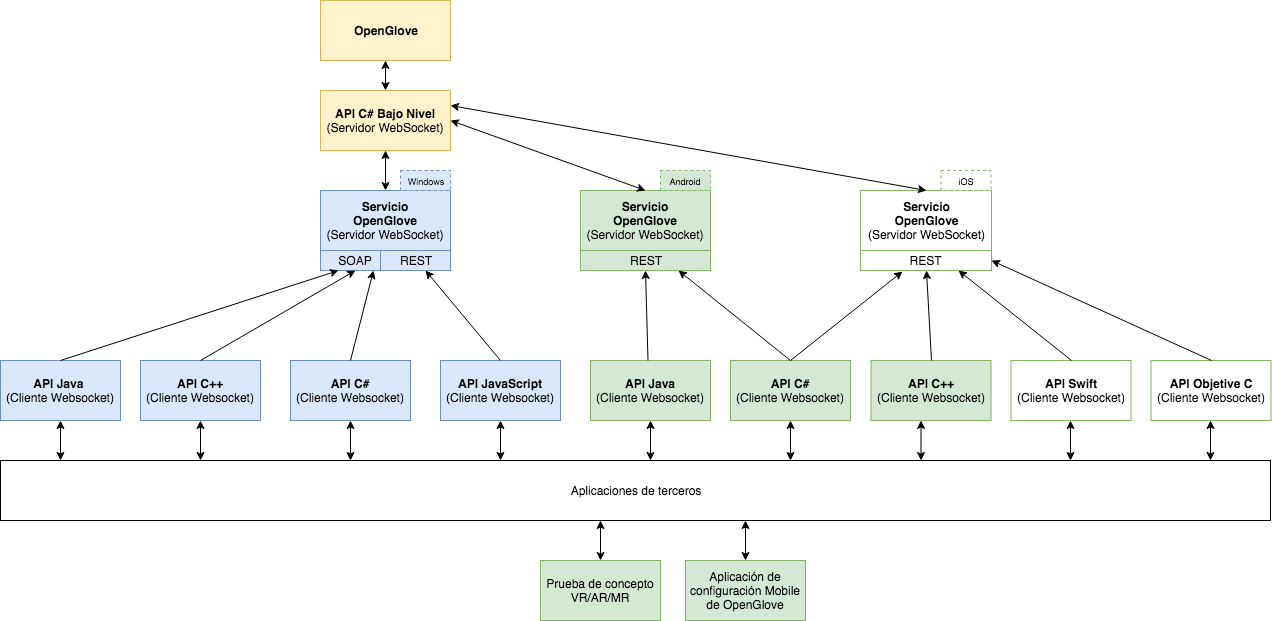
\includegraphics[width=0.9\textwidth]{images/chapter01/OpenGlove-Architecture-02.png} 
    \caption[Arquitectura Openglove]{Arquitectura OpenGlove \\Fuente: Elaboración propia (2018)}
    \label{fig:propuesta-arquitectura-open-glove}
  \end{center}
\end{figure}

\subsection{Propósitos de la solución}
%Propósito de la solución: Se indica el propósito del producto del proyecto, la razón que justificaría la existencia de una solución. Corresponde a la visión que tiene en mente el cliente respecto de la situación futura, o el beneficio que se espera reciba el destinatario de la solución, indicando en qué medida mejoraría la situación actual del problema.
El propósito del proyecto es poner al alcance de distintas comunidades las herramientas para el desarrollo y uso de dispositivos de respuesta vibrotáctil y seguimiento de las manos en ambientes de realidad virtual, mixta y aumentada, junto con promover el uso de OpenGlove en la comunidad Android, los entusiastas del DIY (Do It Yourself)  o ``házlo tú mismo'' y fabricantes que quieran hacer uso de estas tecnologías para sus proyectos.
    \section{Objetivos y alcance del proyecto}

\subsection{Objetivo general}

El objetivo general del proyecto es desarrollar un SDK que permita dar soporte a OpenGlove en dispositivos móviles.

%El objetivo general del proyecto es desarrollar una aplicación móvil que permita dar soporte a OpenGlove en dispositivos móviles, como así también desarrollar un SDK que permita la integración con aplicaciones de terceros mediante API.

\subsection{Objetivos específicos}

%Objetivos específicos: Especifican resultados parciales o metas intermedias necesarias para la consecución del objetivo general. Cada objetivo logrado se debe poder evaluar (los resultados son mensurables). Estos objetivos no deben ser confundidos con los propósitos del producto del trabajo. Numerar secuencialmente cada uno de los objetivos para poder identificarlos y así poder referirse a ellos.
En esta sección se listan los resultados parciales definidos para lograr el objetivo general del proyecto de titulación.

\begin{enumerate}
\item Desarrollar la aplicación de configuración de OpenGlove en Android. Permitiendo la creación, visualización, actualización y eliminación de los perfiles de configuración.

\item Desarrollar APIs en Java y C\# que permitan la administración de dispositivos Bluetooth en segundo plano en Android permitiendo la conexión, desconexión, activación y listado de guantes OpenGlove.  También permitirá la activación y control de actuadores \footnote{Definición actuadores: Un actuador es un dispositivo inherentemente mecánico cuya función es proporcionar fuerza para mover o “actuar” otro dispositivo mecánico. Dependiendo de el origen de la fuerza el actuador se denomina ``neumático'', ``hidráulico'' o ``eléctrico'' \citep{actuadores}}, flexores \footnote{  ``... es un sensor de flexión que produce una resistencia variable en función del grado al que este doblada".\citep{flexor-sensor-01}} e IMU (\textit{Inertial Measurement Unit}).

%\item Implementar la autenticación mediante cuentas de Google para acceder a los perfiles de configuración en FireBase \footnote{Base de datos no relacional en la nube Firebase \url{https://firebase.google.com/?hl=es-419}}.

\item Realizar evaluaciones de rendimiento para las APIs Java y C\#.

\item Demostrar el uso del SDK en un ambiente de VR, AR o MR, utilizando las APIs desarrolladas.
\end{enumerate}



    \section{Metodologías y herramientas utilizadas}

%
En esta sección se presenta la metodología utilizada a lo largo del proyecto, las herramientas y el ambiente de desarrollo del SDK que permitirá el soporte de OpenGlove en dispositivos móviles.

\subsection{Metodología a usar}
Para alcanzar los objetivos planteados en este proyecto, también es necesario elegir una metodología adecuada para el proyecto. En base a esto y a la incertidumbre que presenta el proyecto, es necesario que se elija una metodología que reduzca los riesgos asociados,  permitiendo entregas de software funcional de manera rápida y que puedan ser validados por el cliente (profesor guía). En este contexto y dado que el proyecto de título debe ser realizado dentro del semestre considerando un trabajo de 612 horas cronológicas y basado en la experiencia y el desarrollo de proyectos de similares características, la metodología planteada a continuación es la adecuada para el presente proyecto de ingeniería propuesto. 

La metodología corresponde a la utilizada por el grupo de investigación y desarrollo InTeracTion. Puede separarse en dos etapas principales. La primera etapa consiste en el desarrollo de prototipos funcionales, con la finalidad de obtener retroalimentación del cliente y así cubrir los requerimientos del cliente de manera iterativa. Esta etapa tiene como referencia la metodología RAD (Rapid Application Development) \citep{Martin:1991:RAD:103275}, la cual está orientada a grupos pequeños, enfocada en el producto y no en la documentación generada, necesitando entregas rápidas para obtener retroalimentación del producto desechable desarrollado.  El prototipo final aprobado será la base con lo que se desarrollará la siguiente etapa. La segunda etapa consiste en el desarrollo de las funcionalidades requeridas para el producto, utilizando como base el prototipo funcional de la primera etapa. El proyecto se desarrolla de manera iterativa e incremental, para su gestión se establece  como mínimo una reunión semanal en la cual se tratan temas como  el estado de avance, los compromisos asumidos para la semana, los compromisos siguientes y los problemas ocurridos.  En estas reuniones es posible tomar decisiones sobre los problemas ocurridos y cambiar de estrategia según sea necesario, esto permite reducir los riesgos ocasionados por la incertidumbre del proyecto. 

%<metodología del profesor Roberto>
En resumen la metodología a utilizar contempla las siguiente características:
\begin{itemize}
\item Primera etapa de desarrollo mediante prototipos basada en RAD.
\item Segunda etapa de desarrollo iterativo del prototipo maduro y aceptado.
\item Como mínimo reuniones una vez a la semana en todas las etapas.
\end{itemize}

Para la gestión del proyecto se utilizan los siguientes recursos, que permiten tener un seguimiento del trabajo a realizar, :

\begin{itemize}
\item Kanban físico y compromisos semanales.
\item Kanban simple de tres columnas o estados por hacer (TO DO), haciendo (DOING) y hecho (DONE).
\end{itemize}

%</metodología del  profesor Roberto>

Para que el proyecto llegue a buen término, se debe elegir la metodología adecuada al proyecto dado el contexto del mismo. Dada las características y la interacción que se desea establecer con el profesor guía como cliente, se adoptó la metodología utilizada por InTeracTion. Además, esta metodología presenta ventajas por sobre las tradicionales respecto de la adaptabilidad, colaboración con el cliente y entregas funcionales iterativas que pueden ser evaluadas cada cierto tiempo, mostrando los avances y favoreciendo el producto funcionando por sobre la documentación exhaustiva \footnote{Manifiesto ágil: \url{http://agilemanifesto.org/}}.

\subsection{Herramientas de Software}
En esta sección se listan las herramientas de Software que se utilizaron para el desarrollo del proyecto de título.
La aplicación fue desarrollada utilizando el IDE Visual Studio Community 2018 para Mac \footnote{Xamarin más VS Community para Mac 2018: \url{https://store.xamarin.com/}} en conjunto con el ecosistema de plataformas para compilar \footnote{ En resumidas palabras un compilador es un programa informático que traduce un programa escrito en un lenguaje de programación a otro lenguaje de programación. % Usualmente el segundo lenguaje es lenguaje de máquina, pero también puede ser un código intermedio (bytecode), o simplemente texto.
Este proceso de traducción se conoce como compilación. \url{http://www.ictea.com/cs/knowledgebase.php?action=displayarticle&id=8817}} aplicaciones móviles Xamarin.Forms, el cual utiliza el lenguaje de programación C\# para el desarrollo de aplicaciones nativas multiplataforma. Adicionalmente se utilizó el IDE Android Studio \footnote{Android Studio: \url{https://developer.android.com/studio/index.html?hl=es-419}}, el cual corresponde al IDE oficial para el sistema operativo Android, el cual integra distintas herramientas de desarrollo, como el SDK de Android, el editor de texto, el soporte para control de versiones, compilador, etc. A continuación se listan otras herramientas de software para el apoyo para el desarrollo del proyecto.

\begin{enumerate}

\item Github\footnote{Github: \url{https://github.com/}} para el control de  versiones.

\item Texmaker \footnote{Texmaker : \url{http://www.xm1math.net/texmaker/}}, para la escritura de la memoria.

\item RStudio\footnote{Rstudio: \url{https://www.rstudio.com/}}: para el análisis de datos de la evaluación del proyecto.

\item Google Drive\footnote{Google Drive: \url{https://www.google.com/intl/es\_ALL/drive/}}, para generar y compartir documentos  y archivos de manera colaborativa.

\item Microsoft Project Professional y Gantter, para el desarrollo de la carta gantt del proyecto de título.

\end{enumerate}

\subsection{Herramientas de Hardware}
El ambiente de desarrollo en el cual se desarrolló SDK fue un Macbook Pro con las siguientes características:
\begin{enumerate}
\item Sistema operativo SO macOS Sierra versión 10.13.3.
\item Procesador Intel Core i5,  3,1 GHz .
\item  Memoria RAM 8GB 2133 MHz LPDDR3.
\item 512 GB disco duro SSD.
\item Gráficos Intel Iris Plus Graphics 650 1536 MB.
\end{enumerate}
Las pruebas de la aplicación se realizarán utilizando Android Virtual Device (AVD) mediante Android Studio  y un smartphone \textit{Samsung Galaxy  S5 mini} \footnote{Smartphone: \url{http://www.movilcelular.es/samsung-galaxy-s5-mini-duos-sm-g800h/caracteristicas/1659}} con las siguientes características:

\begin{enumerate}
\item Sistema Operativo Android Marshmallow 6.0.1.
\item CPU: 1.4Ghz Quad-Core ARM Cortex-A7.
\item GPU: ARM Mali-400 MP4 450Mhz.
\item Memoria RAM 1,5GB LPDDR2.
\item Almacenamiento interno 16GB (12GB accesible al usuario).
\item Bluetooth Versión 4.0 con A2DP.
\item Sensores:  Acelerómetro, Proximidad, Brújula , Luz ambiental, Giroscopio, Biométrico (huellas digitales).
\end{enumerate}

El prototipo de dispositivo OpenGlove disponible en InTeracTion fue utilizado para realizar las pruebas y el desarrollo del SDK. Se usaron el IMU, motores y sensores de flexibilidad disponibles en el prototipo.

\begin{enumerate}
\item Sensores de flexibilidad de 2,2”, SparkFun.
\item Sensor de rastreo IMU, SparkFun.
\item Actuadores (En específico motores de vibración).
\item Bluetooth mate silver, Sparkfun.
\end{enumerate}
    \section{Organización del documento}

% cuidado con la palabra implementar (es implementar o desarrollar)

El presente documento posee seis capítulos que abarcan la totalidad de este proyecto de desarrollo en sus distintas fases. El Capítulo 1, Introducción, incluye los antecedentes y motivación del proyecto, presentando el problema y solución propuesta junto con los objetivos necesarios para concretarla. El Capítulo 2, Marco teórico, introduce los conceptos relevantes que permitirán una mejor compresión del problema junto a su solución. También se incluye el estado del arte, el cual detalla las soluciones alternativas actuales del problema planteado, detallando y comparándolas entre ellas. En el Capítulo 3, Análisis, se realiza un análisis sobre el desarrollo del SDK analizando los componentes de hardware y software disponibles, generando prototipos hasta que se genere el producto esperado. Luego en el Capítulo 4, Diseño e implementación, se diseña la solución a nivel de mockups  o maquetas, también a nivel arquitectural, comportamiento y de protocolos de comunicación. Posteriormente se implementan para lograr la solución diseñada. El Capítulo 5, Evaluación técnica, se realiza una evaluación del software desarrollado para establecer cuáles son los tiempos de respuesta (latencia) presentes y la comparativa con la versión de escritorio. Además se considera otro factor importante respecto a la solución , esto es, la eficiencia energética de la misma. Por último,  en el Capítulo 6, Conclusiones, se detallan los objetivos cumplidos, también los resultados obtenidos con la solución, los alcances y limitaciones de la misma, posibles mejoras para trabajos futuros y observaciones finales pertinentes.
    
\newpage
\chapter{Marco teórico}
%El presente capítulo da cuenta de los fundamentos teóricos y prácticos de este trabajo. En primer lugar, se presenta un marco conceptual y luego se presenta una revisión del estado del arte.
Este capítulo permite establecer las bases teóricas necesarias para una mejor comprensión del presente documento. El capítulo se divide en tres secciones, la primera correspondiente al Marco conceptual, en el cual se establecen los conceptos bases pertinentes al proyecto, luego en el Estado del arte se realiza una revisión del mismo.
	\section{Marco conceptual}

\subsection{API}

\subsection{SDK}

\subsection{Haptics}

\subsection{Tipos de aplicaciones móviles}
%https://www.solbyte.com/blog/2014/07/21/tipos-de-aplicaciones-moviles-nativas-webs-hibridas/

%https://clearbridgemobile.com/mobile-app-development-native-vs-web-vs-hybrid/

% Very : https://www.mobiloud.com/blog/native-web-or-hybrid-apps/

	\subsubsection{Nativas}
	
	\subsubsection{Híbridas}
	
	\subsubsection{Web}




    \section{Estado del arte}
%Estado del arte: El estado del arte de un objeto de estudio se refiere al estado más elevado de desarrollo alcanzado por el objeto en un momento particular. En este caso el objeto de estudio es la solución del problema, que puede ser un producto de software, un método, un modelo, una teoría, etc. Se presenta el ámbito o la(s) principal(es) disciplina(s) que aborda(n) soluciones al problema (redes neuronales, informática médica, seguridad en redes, sistemas cooperativos, industria informática, etc.). Se espera una revisión de los fundamentos teóricos del objeto de estudio, los antecedentes que hay del tema expresado en dos formas, primero una breve descripción de su evolución y luego una descripción resumida del estado del arte actual (últimos años), desde dos perspectivas: nacional e internacional. Lo más importante es el estado del arte al día de hoy.

En esta sección se busca presentar los antecedentes y el estado actual sobre los dispositivos de retroalimentación vibrotáctil disponibles en el mercado, las cuales suelen venir con herramientas para el desarrollo de aplicaciones de terceros. Una de las herramientas que se le suelen facilitar a los desarrolladores es el SDK (\textit{Software Development Kit}), el cual es un conjunto de herramientas utilizadas para desarrollar aplicaciones proporcionadas por proveedores de hardware y software. Los SDK suelen estar compuestos por interfaces de programación de aplicaciones APIs (\textit{Application Program Interface}), código de muestra, documentación, entre otros elementos \citep{techopedia-SDK}. En la Tabla \ref{table:SDKs} muestra una comparativa de distintas características de los SDKs del mercado referente a dispositivos de \textit{haptic feedback}. Es importante señalar que el SDK no posee soporte multiplataforma, tampoco tiene una integración directa con Unity, sería necesario hacer un plugin para ello.

% ... /table-generation/sdk-comparation.tgn
\begin{table}[H]
\centering
\caption[Comparación SDK de distintos Guantes]{Comparación SDK de distintos Guantes \\Fuente: Elaboración propia (2018)}
\label{table:SDKs}
\begin{tabular}{|l|l|l|l|l|}
\hline
          & \begin{tabular}[c]{@{}l@{}}Lenguajes \\ soportados\end{tabular} & SO soportado                                                                  & \begin{tabular}[c]{@{}l@{}}Información \\ Bidireccional\end{tabular} & \begin{tabular}[c]{@{}l@{}}Integración \\ SDK con Unity\end{tabular} \\ \hline
OpenGlove & C\#, Java, JavaScript                                           & Windows                                                                       & SI                                                                   & \begin{tabular}[c]{@{}l@{}}NO\\ (Requiere plugin)\end{tabular}       \\ \hline
GloveOne  & C++ y C\#                                                       & \begin{tabular}[c]{@{}l@{}}Windows, MAC, \\ Linux, Android e iOS\end{tabular} & SI                                                                   & SI                                                                   \\ \hline
AvatarVR  & C++ y C\#                                                       & \begin{tabular}[c]{@{}l@{}}Windows, MAC,\\ Linux, Android e iOS\end{tabular}  & SI                                                                   & SI                                                                   \\ \hline
Dexmo     & No anunciado                                                    & No anunciado                                                                  & SI                                                                   & Si                                                                   \\ \hline
\end{tabular}
\end{table}


\subsection{OpenGlove}
	Es un proyecto que consiste en un dispositivo que entrega \textit{haptics feedback}. Fue pensado para dispositivos de realidad virtual e interfaces naturales. El proyecto partió en el 2014 con el propósito  de facilitar la construcción y flexibilizar uno de los recursos claves para la inmersión en ambientes de  realidad virtual \citep{openglove-info-page}. OpenGlove se ha pensado para que pueda ser utilizado en conjunto con otros dispositivos, como Oculus Rift, Kinect y Leap Motion. Por otra parte, los prototipos de OpenGlove, utilizan motores configurables con diferentes niveles de potencia, lo que permite la respuesta vibrotáctil en distintas áreas de la mano. Esto puede ser utilizado para representar la sensación de tocar objetos en entornos virtuales, como también, recibir retroalimentación que represente impacto, el cual sería útil en un juego de boxeo por ejemplo.   Actualmente, se soporta el uso de actuadores, sensores de flexibilidad y Unidad de Medición Inercial (IMU por sus siglas en inglés).
    
            
\begin{figure}[H]
  \begin{center} 
   	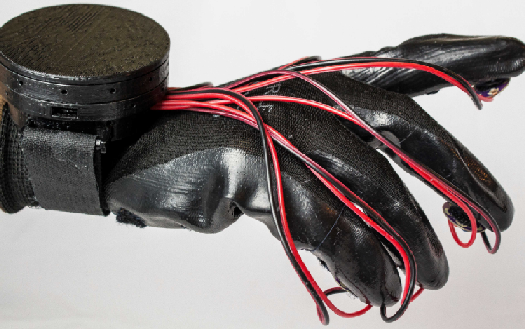
\includegraphics[width=0.5\textwidth]{images/fig-analisis-solucion/openglove.png} 
    \caption[Guantes OpenGlove]{Guantes OpenGlove \\Fuente: \cite{openglove-info-page}} 
    \label{fig:OpenGlove}
  \end{center}
\end{figure}

%\subsection{GloveOne}
% Now neurodigital only sell AvatarVR versión
%	Es un guante diseñado por Neurodigital para ofrecer la sensación del contacto con objetos en entornos de realidad virtual mediante  \textit{haptic feedback}. Posee 10 actuadores  vibrotáctiles distribuidos en posiciones fijas en los dedos, posee cinco sensores flexibles para el seguimiento de los dedos, se conecta mediante Bluetooth 4.0, posee una batería de litio con una duración de 8 horas. El guante posee un costo que van desde los 299 \euro \space . Las licencias profesionales alcanzan precios desde los  3.300 \euro \space hasta 13.300 \euro  \space la versión premium,  permiten acceder a la documentación, SDK y soporte, entre otros servicios.  \footnote{Precio de GloveOne y licencias: \url{https://www.neurodigital.es/gloveone/}}
    

%\begin{figure}[H]
%  \begin{center} 
%   	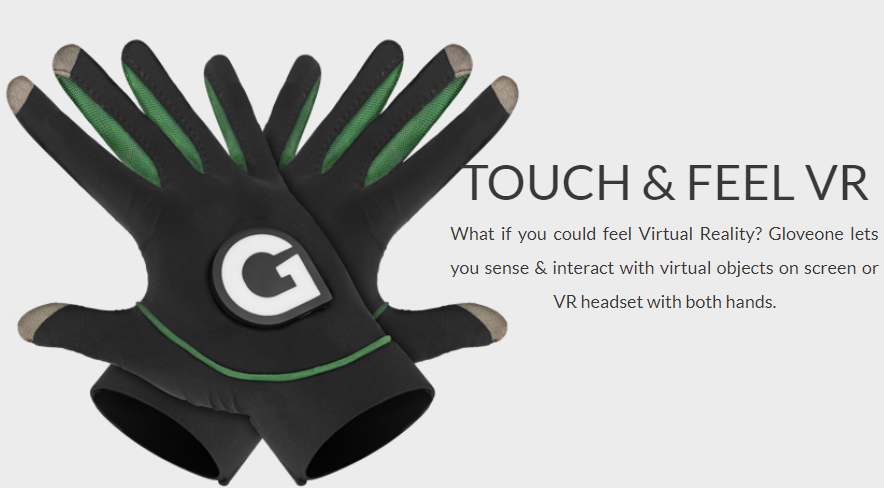
\includegraphics[width=0.4\textwidth]{images/fig-analisis-solucion/globeone.png} 
 %   \caption[Guantes GloveOne]{Guantes GloveOne \\Fuente: \cite{gloveone-info-page}} 
 %  \label{fig:gloveone}
 % \end{center}
%\end{figure}

    
\subsection{AvatarVR}
    	AvatarVR es otro guante diseñado por Neurodigital e incluye todas las funcionalidades presentes en GloveOne, junto a unas capacidades adicionales que ofrecen más funcionalidades. Además de los guantes se incluye un accesorio llamado TrackBand, que permite la captura de movimiento de la parte superior del cuerpo, basada en una configuración minimalista de los sensores  para en brazos y manos. Además sensores para el seguimiento de dedos mediante sensores 6x 9-AXIS IMUs. El guante y las trackbands poseen un costo desde 1.100 \euro \space.  Las licencias son de dos tipos profesional a 3.300 \euro \space y premium  a 13.300 \euro  \space para acceder a la documentación, SDK, soporte, entre otros servicios. 
	\footnote{Precio AvatarVR y licencias: \url{https://www.neurodigital.es/avatarvr/}}
        
\begin{figure}[H]
  \begin{center} 
   	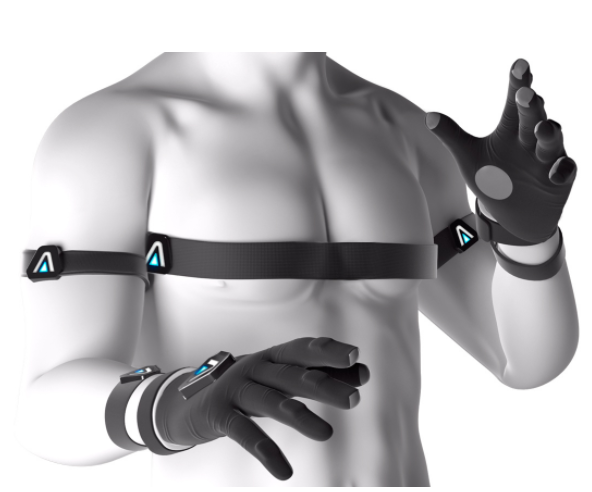
\includegraphics[width=0.4\textwidth]{images/fig-analisis-solucion/avatar-VR.png} 
     \caption[Guantes AvatarVR y TrackBand]{Guantes AvatarVR y TrackBand \\Fuente: \cite{avatarvr-info-page}} 
    \label{fig:avatarVR}
  \end{center}
\end{figure}

        
\subsection{Dexmo} 
    Dexmo es un exoesqueleto que permite \textit{haptic feedback} en ambientes de realidad virtual. Esto lo logra mediante la capacidad de retroalimentación de fuerza, lo que permite al usuario sentir el tamaño y la forma de cualquier objeto digital, lo que mejora enormemente la inmersión. La rigidez variable se logra mediante un control preciso del motor. Con esta característica, cada objeto virtual puede tener su propia rigidez.
    
Por protección de propiedad intelectual, su SDK sólo es accesible a clientes que hayan comprado Dexmo DK1. %En la figura se aprecian las capturas de lo que contiene sería una vista previa de su SDK.
    
            
\begin{figure}[H]
  \begin{center} 
   	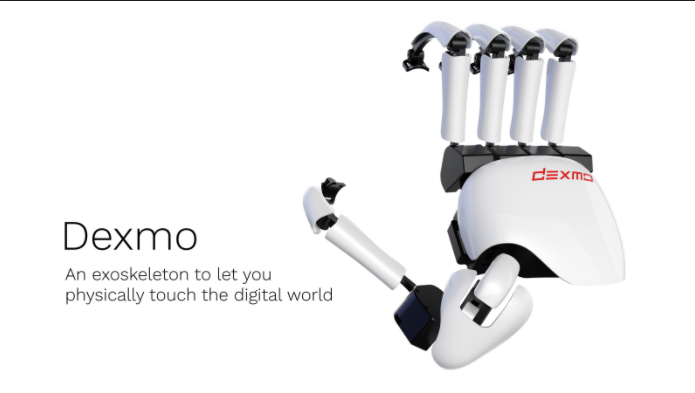
\includegraphics[width=0.5\textwidth]{images/fig-analisis-solucion/dexmo.png} 
    \caption[Guantes Dexmo]{Guantes Dexmo \\Fuente: \cite{dexmo-info-page}}  
    \label{fig:dexmo}
  \end{center}
\end{figure}
    
\subsection{Manus VR}
	Manus VR es un guante que permite \textit{haptic feedback}, seguimiento de dedos y manos para ambientes de realidad virtual. Sus especificaciones comerciales establecen que, es lavable, permite el seguimiento de los brazos, que también incluye un IMU para medir la orientación de la mano. Manus VR puede ser adquirido en dos versiones, la de desarrollador con un precio de 1.990 \euro \space y una versión profesional con un precio de 4.990 \euro \space \footnote{Precio de Manus VR y licencias \url{https://manus-vr.com/order.php}}
    
\begin{figure}[H]
  \begin{center} 
   	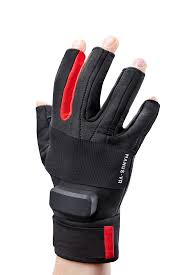
\includegraphics[width=0.3\textwidth]{images/fig-analisis-solucion/manus-vr.jpeg} 
    \caption[Guantes Manus VR]{Guantes Manus VR \\Fuente: \cite{manusvr-info-page}} 
    \label{fig:manus-vr}
  \end{center}
\end{figure}

\subsection{Haptx}
%Este es nuevo, muy interesante ...
%“HaptX Gloves are the result of years of research and development in haptic technology,” said Jake Rubin, Founder and CEO, HaptX Inc. “What really sets HaptX Gloves apart is the unprecedented realism they deliver. Our patented microfluidic technology physically displaces the skin the same way a real object would when touched, closely replicating its texture, shape, and movement.” 
\footnote{ Haptx \url{https://haptx.com/}}

\subsection{Sense glove}
\footnote{Sense Glove: \url{https://www.senseglove.com/}}

\subsection{Virtual Reality Smart Glove}
\footnote{VR Smart Glove: \url{http://www.designpartners.com/projects/virtual-reality-smart-glove/
}}


    \section{Resumen}
OpenGlove es un proyecto Open Source\footnote{ ``Open source o código abierto es el término empleado al software distribuido bajo una licencia que permite al usuario acceso al código fuente. Este tipo de licencia posibilita el estudio y la modificación del software con total libertad. Además, su redistribución está permitida siempre y cuando esta posibilidad vaya en concordancia con los términos de licencia bajo la que se adquiere el software" \citep{open-source}.}  que permite la retroalimenación vibrotáctil y comunicación bidireccional entre el guante y las aplicaciones mediante el uso del protocolo WebSocket. Como se ha podido ver, existen diversas alternativas en el mercado de dispositivos hápticos, siendo OpenGlove la alternativa Open Source que no requiere de costos altos de licencias ni del guante,  el cual es desarrollado según las necesidades específicas requeridas. Para lograr que la comunidad de desarrolladores de VR/AR/MR pueda integrar OpenGlove en entornos móviles y realizar una fácil configuración de ellos, se desarrollará un SDK que incluye las APIs de alto nivel necesarias para el desarrollo en las plataformas móviles, la aplicación de configuración y la documentación de uso de las APIs en pruebas de concepto. Es importante señalar la importancia de las pruebas de rendimiento sobre la solución a desarrollar. esto toma relevancia cuando se busca disminuir la latencia de los dispositivos conectados. Esto se debe considerar para brindar una excelente experiencia en entornos virtuales sin que se presenten retardos perceptibles. 

%El creciente mercado y comunidad de desarrolladores de VR, AR y MR, favorece la adopción de estas tecnologías en el tiempo.

\newpage
\chapter{Análisis}
%en este capítulo ....
En este capítulo se realiza un levantamiento de requisitos funcionales y no funcionales del SDK a desarrollar, considerando el estado actual del proyecto. Para luego realizar los diferentes prototipos de software basados en la metodología RAD, hasta obtener un producto final que cumpla con todos los requisitos establecidos en un comienzo. 
	\section{Levantamiento de requisitos de software}

\subsection{Antecedentes}
%debería incluirse los requerimientos de las anteriores 2 tesis (en lo que respecta al software) debe especificarse
% trabajo relacionado al SDK alto nivel (extensión de software)
% trabajo relacionado al extensión de OpenGlove a nivel de Hardware y Software
En los trabajos anteriores relacionados a OpenGlove, realizados por \cite{tesis-monsalve-rodrigo}, \cite{tesis-meneses-sebastian} y \cite{tesis-cerda-rodrigo} se ha logrado establecer las bases de hardware y software para dar soporte a la retroalimentación vibrotáctil y el seguimiento de las manos. En el trabajo de \cite{tesis-meneses-sebastian}, se realizó una extensión de sofware a OpenGlove, desarrollando un SDK de alto nivel para la retroalimentación vibrotáctil. Por otra parte, el trabajo de \cite{tesis-cerda-rodrigo}, se realizó una extensión de software y hardware para la captura de movimientos de la mano. En base a estos dos últimos se desprenden las diferentes funcionalidades y soporte que se debe lograr a nivel de software, para dar soporte a los actuadores, sensores de flexibilidad e IMU. Actualmente OpenGlove cuenta con un SDK para Windows, el cual incluye el sofware de configuración y cuatro APIs de alto nivel para los lenguajes C\#, Java, C++ y JavaScript. El SDK fue desarrollado en el IDE Visual Studio.

%Los dispositivos móviles suelen tener menos capacidades de cálculo, memoria y batería, por lo que se esperan tener latencias mayores a las presentadas en los trabajos antes mencionados. El SDK para dispositivos móviles


\subsection{Requisitos}
% ¿Requisitos o Requerimientos? http://investigacionit.com.ar/es/requisitos-o-requerimientos/
% Especificación de Requisitos según el estándar de IEEE 830 https://www.fdi.ucm.es/profesor/gmendez/docs/is0809/ieee830.pdf

Al realizar un análisis de los antecedentes y el problema planteado en el Capítulo 1, se capturan los siguientes requisitos funcionales del software.

%%%%%%%%%%%%%%%%%%%%%%%%%%%%%%%%%%%%%%%%%%%%
% https://www.tablesgenerator.com/
%\caption[Requisitos funcionales de software]{Requisitos funcionales de software \\ Fuente: Elaboración propia (2018)}
%\label{table:RF}\\

%{START} .../latex-2018-OpenGlove-SDK/tables-generator/functional-requeriments

% Please add the following required packages to your document preamble:
% \usepackage{longtable}
% Note: It may be necessary to compile the document several times to get a multi-page table to line up properly
\begin{longtable}[c]{|l|l|l|l|}
\caption[Requisitos funcionales de software]{Requisitos funcionales de software \\ Fuente: Elaboración propia (2018)}
\label{table:RF}\\
\hline
ID & Síntesis del Requisito & Descripción & Origen \\ \hline
\endfirsthead
%
\endhead
%
RF001 & \begin{tabular}[c]{@{}l@{}}El sistema debe permitir\\ al usuario ver los\\ dispositivos OpenGlove\\ emparejados\end{tabular} & \begin{tabular}[c]{@{}l@{}}El sistema debe ofrecer una \\ recopilación de los dispositivos \\ OpenGlove emparejados con\\ el dispositivo móvil, su estado de \\ conexión actual y la dirección \\ MAC del mismo.\end{tabular} & \begin{tabular}[c]{@{}l@{}}Inicio,\\ modificado de\\ Meneses (2016)\end{tabular} \\ \hline
RF002 & \begin{tabular}[c]{@{}l@{}}El sistema debe permitir\\ al usuario definir la\\ configuración de\\ hardware de cada guante\end{tabular} & \begin{tabular}[c]{@{}l@{}}Cada placa LilyPad posee pines \\ programables, en los cuales el \\ usuario puede conectar actuadores,\\ sensores de flexibilidad e IMU \\ para crear su propio OpenGlove. \\ Es necesario que se establezca\\ esta configuración en el sistema\\ para cada guante, ya que de ella \\ depende la activación de actuadores\\ y la lectura de datos de los flexores\\ e IMU. Se debe diferenciar pines\\ digitales y análogos de la placa\\ Arduino\end{tabular} & \begin{tabular}[c]{@{}l@{}}Inicio,\\ modificado de\\ Meneses (2016)\\ y RF001 de\\ Cerda (2017)\end{tabular} \\ \hline
RF003 & \begin{tabular}[c]{@{}l@{}}El sistema debe permitir\\ al usuario guardar una\\ configuración de\\ hardware\end{tabular} & \begin{tabular}[c]{@{}l@{}}Al crear un nuevo perfil de hardware\\ para un guante, el sistema debe contar\\ con un mecanismo para la persistencia\\ de esta configuración.\end{tabular} & \begin{tabular}[c]{@{}l@{}}Inicio,\\ Meneses (2016)\end{tabular} \\ \hline
RF004 & \begin{tabular}[c]{@{}l@{}}El sistema debe permitir\\ al usuario abrir una\\ configuración de\\ hardware previamente\\ almacenada por el\\ sistema\end{tabular} & \begin{tabular}[c]{@{}l@{}}Una vez guardada una configuración,\\ esta debe ser reconocible por el \\ sistema para su uso posterior en otro\\ guante.\end{tabular} & \begin{tabular}[c]{@{}l@{}}Inicio,\\ Meneses (2016)\end{tabular} \\ \hline
RF005 & \begin{tabular}[c]{@{}l@{}}El sistema debe permitir\\ al usuario definir la\\ configuración de \\ actuadores de cada\\ guante\end{tabular} & \begin{tabular}[c]{@{}l@{}}Dependiente de la configuración de\\ hardware, la configuración de\\ actuadores es una representación de\\ la distribución física de los actuadores\\ LilyPad en una  mano virtual. Esta\\ representación permite establecer\\ mapeos región-actuador usables en\\ una API de alto nivel. Se debe ofrecer\\ al usuario una solución gráfica que\\ permita ordenar la posición de los\\ actuadores en una representación de\\ la mano. También debe permitir la\\ posibilidad de agregar su propia\\ imagen que represente el mapeo.\end{tabular} & \begin{tabular}[c]{@{}l@{}}Inicio, \\ modificado de\\ Meneses (2016)\end{tabular} \\ \hline
RF006 & \begin{tabular}[c]{@{}l@{}}El sistema debe permitir\\ al usuario guardar una\\ configuración de \\ actuadores\end{tabular} & \begin{tabular}[c]{@{}l@{}}Al crear un nuevo perfil de actuadores\\ para un guante, el sistema debe contar\\ con un mecanismo para la persistencia\\ de estaconfiguración.\end{tabular} & \begin{tabular}[c]{@{}l@{}}Inicio,\\ Meneses (2016)\end{tabular} \\ \hline
RF007 & \begin{tabular}[c]{@{}l@{}}El sistema debe permitir\\ al usuario abrir una \\ configuración de\\ actuadores previamente\\ almacenada por el\\ sistema\end{tabular} & \begin{tabular}[c]{@{}l@{}}Una vez guardada una configuración\\ de actuadores, esta debe ser\\ reconocible por el sistema para su uso\\ posterior en otro guante.\end{tabular} & \begin{tabular}[c]{@{}l@{}}Inicio,\\ Meneses (2016)\end{tabular} \\ \hline
RF008 & \begin{tabular}[c]{@{}l@{}}El sistema debe permitir\\ al usuario establecer\\ conexión con un \\ dispositivo OpenGlove\\ emparejado\end{tabular} & \begin{tabular}[c]{@{}l@{}}Una vez emparejado un guante\\ OpenGlove, el sistema debe permitir\\ que el usuario inicie la conexión\\ Bluetooth. No es necesario que el\\ usuario especifique la dirección\\ MAC del guante.\end{tabular} & \begin{tabular}[c]{@{}l@{}}Inicio,\\ modificado de \\ Meneses (2016)\end{tabular} \\ \hline
RF009 & \begin{tabular}[c]{@{}l@{}}El sistema debe permitir\\ al usuario activar una \\ región de un guante con\\ intensidad a voluntad\end{tabular} & \begin{tabular}[c]{@{}l@{}}El sistema debe exponer al usuario\\ una sección que le permita activar\\ una región de un guante con la\\ intensidad (entre 0 y 255) que él\\ desee para probar el hardware. Esta\\ región esta predefinida y debe ser\\ independiente de la configuración\\ de hardware (actuadores) presente\\ en el guante. Esta función debe\\ estar disponible para uno o varios\\ actuadores en un guante.\end{tabular} & \begin{tabular}[c]{@{}l@{}}Inicio,\\ modificado de\\ Meneses (2016)\end{tabular} \\ \hline
RF010 & \begin{tabular}[c]{@{}l@{}}El sistema debe permitir\\ al usuario operar con\\ distintas implementa-\\ ciones de OpenGlove\end{tabular} & \begin{tabular}[c]{@{}l@{}}Al momento de crear un nuevo\\ perfil de hardware, el sistema\\ debe proveer un mecanismo para\\ que el usuario genere su propia\\ placa, lo que se traduce en un\\ nombre y una cantidad de pines\\ para poder usarla en su\\ configuración.\end{tabular} & \begin{tabular}[c]{@{}l@{}}Inicio,\\ Meneses (2016)\end{tabular} \\ \hline
RF011 & \begin{tabular}[c]{@{}l@{}}El sistema actual debe\\ permitir al usuario\\ guardar y cargar una\\ configuración de\\ hardware incluyendo\\ los flexores\end{tabular} & \begin{tabular}[c]{@{}l@{}}El SDK debe ser capaz de guardar\\ y cargar una configuración de\\ hardware, compuesta por  actuadores\\ y/o sensores de flexibilidad.\end{tabular} & \begin{tabular}[c]{@{}l@{}}Inicio,\\ modificado de\\ Cerda (2017)\end{tabular} \\ \hline
RF012 & \begin{tabular}[c]{@{}l@{}}El sistema debe permitir\\ al usuario crear una\\ configuración de los\\ sensores de flexibilidad\\ y del sensor de rastreo\\ IMU\end{tabular} & \begin{tabular}[c]{@{}l@{}}El software debe ser capaz de dar\\ soporte para la creación de nuevas\\ configuraciones de los sensores de\\ flexibilidad y el IMU.\end{tabular} & \begin{tabular}[c]{@{}l@{}}Inicio,\\ modificado de \\ Cerda (2017)\end{tabular} \\ \hline
RF013 & \begin{tabular}[c]{@{}l@{}}El sistema debe permitir\\ al usuario seleccionar\\ un sensor de flexibilidad\\ y  relacionarlo a una\\ región del guante\end{tabular} & \begin{tabular}[c]{@{}l@{}}La configuración correspondiente\\ a los sensores de flexibilidad, debe\\ ser capaz de seleccionar una región\\ del guante y relacionarlo con un\\ sensor de flexibilidad.\end{tabular} & \begin{tabular}[c]{@{}l@{}}Inicio,\\ Cerda (2017)\end{tabular} \\ \hline
RF014 & \begin{tabular}[c]{@{}l@{}}El sistema debe permitir\\ al usuario eliminar un\\ sensor de flexibilidad\\ de una región del guante\end{tabular} & \begin{tabular}[c]{@{}l@{}}La configuración de los sensores de\\ flexibilidad debe ser capaz de\\ eliminar un flexor de una región del\\ guante, de tal manera que la región\\ quede libre y el flexor pueda asignarse\\ a una nueva región.\end{tabular} & \begin{tabular}[c]{@{}l@{}}Inicio,\\ Cerda (2017)\end{tabular} \\ \hline
RF015 & \begin{tabular}[c]{@{}l@{}}El sistema debe enviar\\ los datos provenientes\\ de los sensores de\\ flexibilidad\\ automáticamente\end{tabular} & \begin{tabular}[c]{@{}l@{}}Cuando un sensor de flexibilidad es\\ asignado a una región del guante, el\\ sistema debe ser capaz de transmitir\\ los datos de dicho sensor de manera\\ automática, especificando el tipo de\\ dato, región y el valor leído.\end{tabular} & \begin{tabular}[c]{@{}l@{}}Inicio,\\ Cerda (2017)\end{tabular} \\ \hline
RF016 & \begin{tabular}[c]{@{}l@{}}El sistema debe parar\\ de enviar los datos \\ provenientes de los \\ sensores de flexibilidad\\ automáticamente\end{tabular} & \begin{tabular}[c]{@{}l@{}}Cuando un sensor de flexibilidad es\\ eliminado de una región del guante,\\ el sistema debe ser capaz de parar la\\ transmisión de datos de  dicho flexor\\  automáticamente.\end{tabular} & \begin{tabular}[c]{@{}l@{}}Inicio,\\ Cerda (2017)\end{tabular} \\ \hline
RF017 & \begin{tabular}[c]{@{}l@{}}El sistema debe permitir\\ al usuario definir un\\ threshold al momento\\ de enviar datos de los \\ sensores de flexibilidad\end{tabular} & \begin{tabular}[c]{@{}l@{}}El guante enviará el dato de un flexor,\\ solo si este dato posee una diferencia\\ mayor o igual al valor definido como\\ threshold, con respecto al último valor\\ enviado por dicho flexor.\end{tabular} & \begin{tabular}[c]{@{}l@{}}Inicio,\\ Cerda (2017)\end{tabular} \\ \hline
RF018 & \begin{tabular}[c]{@{}l@{}}El sistema debe permitir\\ al usuario la opción de \\ calibrar los sensores de \\ flexibilidad\end{tabular} & \begin{tabular}[c]{@{}l@{}}Los datos provenientes de los sensores\\ de flexibilidad deben ser calibrados\\ con respecto al máximo y mínimo\\ valor leído de la articulación de un\\ dedo.\end{tabular} & \begin{tabular}[c]{@{}l@{}}Inicio,\\ Cerda (2017)\end{tabular} \\ \hline
RF019 & \begin{tabular}[c]{@{}l@{}}El sistema debe permitir\\ al usuario probar los\\ sensores de flexibilidad\end{tabular} & \begin{tabular}[c]{@{}l@{}}Luego de asignar uno o más sensores\\ de  flexibilidad a una región del\\ guante, se debe habilitar un botón que\\ permita probar si la  configuración es\\ correcta, visualizando el valor\\ entregado por cada flexor en dicha\\ región.\end{tabular} & \begin{tabular}[c]{@{}l@{}}Inicio,\\ Cerda (2017)\end{tabular} \\ \hline
RF020 & \begin{tabular}[c]{@{}l@{}}El usuario debe permitir\\ al usuario poder obtener\\ datos desde un sensor de\\ rastreo IMU\end{tabular} & \begin{tabular}[c]{@{}l@{}}La configuración correspondiente al\\ sensor de rastreo IMU, debe ser\\ capaz de activar o desactivar el envío\\ de datos de ésta.\end{tabular} & \begin{tabular}[c]{@{}l@{}}Inicio,\\ Cerda (2017)\end{tabular} \\ \hline
RF021 & \begin{tabular}[c]{@{}l@{}}El sistema debe permitir\\ al usuario poder obtener\\ datos crudos o \\ procesados desde\\ el sensor de rastreo IMU\end{tabular} & \begin{tabular}[c]{@{}l@{}}La configuración del sensor de\\ rastreo IMU, debe ser capaz de definir\\ si los datos enviados por ésta son\\ procesados o no.\end{tabular} & \begin{tabular}[c]{@{}l@{}}Inicio,\\ Cerda (2017)\end{tabular} \\ \hline
RF022 & \begin{tabular}[c]{@{}l@{}}El sistema debe permitir\\ al usuario poder probar\\ el sensor de rastreo IMU\end{tabular} & \begin{tabular}[c]{@{}l@{}}Luego de activar el envío de datos del\\ sensor de rastreo IMU, se debe activar\\ un botón que active la visualización de\\ todos los datos entregados por el sensor.\end{tabular} & \begin{tabular}[c]{@{}l@{}}Inicio,\\ Cerda (2017)\end{tabular} \\ \hline
RF023 & \begin{tabular}[c]{@{}l@{}}El sistema debe permitir\\ al usuario calibrar el\\ sensor de rastreo IMU\end{tabular} & \begin{tabular}[c]{@{}l@{}}Los datos provenientes del IMU deben\\ ser calibrados bajo una posición de\\ referencia,  para poder determinar la\\ posición y orientación de la mano.\end{tabular} & Nuevo \\ \hline
\end{longtable}
%{END} tables-generator/functional-requeriments
%%%%%%%%%%%%%%%%%%%%%%%%%%%%%%%%%%%%%%%%%%%%















La Tabla \ref{table:RNF}, muestra los requisitos no funcionales obtenidos mediante las reuniones con el profesor guía. Al igual que lo señalado por \cite{tesis-monsalve-rodrigo}, de esta lista de requisitos para el SDK, se debe dar especial importancia a RNF004, el cual se refiere al umbral de tiempo que no se debe superar para ofrecer la retroalimentación táctil. Experimentos enfocados en medir los los tiempos en que una persona puede percibir inconsistencias entre una interacción táctil con un objeto virtual y un estímulo táctil recibido, obtienen los siguientes resultados: 54 ms para retroalimentación kinestésica \citep{latency-haptic-kinestesic-2004}, 60 ms en estudios de percepción \citep{latency-haptic-perception-2009} y 60 ms simulaciones quirúrgicas simulaciones \citep{latency-visual-haptic-2015}.


%%%%%%%%%%%%%%%%%%%%%%%%%%%%%%%%%%%%%%%%%%%%
% https://www.tablesgenerator.com/
%\caption[Requisitos no funcionales de software]{Requisitos  no funcionales de software \\ Fuente: Elaboración propia (2018)}
%\label{table:RNF}

\begin{table}[H]
\caption[Requisitos no funcionales de software]{Requisitos  no funcionales de software \\ Fuente: Elaboración propia (2018)}
\label{table:RNF}
\begin{tabular}{|l|l|l|l|}
\hline
ID     & Síntesis del requisito                                                    & Descripción                                                                                                                                                                                                                      & Origen \\ \hline
RNF001 & Sistema multiplataforma                                                   & \begin{tabular}[c]{@{}l@{}}El software a desarrollar debe ser ejecutado\\ inicialmente en el sistema operativo Android,\\ sin embargo, el proyecto en un futuro debe \\ poder dar soporte al sistema operativo iOS.\end{tabular} & Inicio \\ \hline
RNF002 & \begin{tabular}[c]{@{}l@{}}Soportar comunicación\\ Bluetooth\end{tabular} & \begin{tabular}[c]{@{}l@{}}El sistema debe ser capaz de comunicarse\\ con los dispositivos OpenGlove mediante \\ Bluetooth Clásico.\end{tabular}                                                                                 & Inicio \\ \hline
RNF003 & Interoperabilidad                                                         & \begin{tabular}[c]{@{}l@{}}El SDK debe permitir la interoperabilidad\\ entre los lenguajes de programación C\# y\\ Java.\end{tabular}                                                                                            & Inicio \\ \hline
RNF004 & Umbral latencia aceptada                                                  & \begin{tabular}[c]{@{}l@{}}El SDK no debe superar el umbral de 60 ms\\ de latencia perceptible por el usuario.\end{tabular}                                                                                                      & Inicio \\ \hline
\end{tabular}
\end{table}

%{START} .../2018Thesis-OpenGloveSDKMobile/tables-generator/no-functional-requeriments



%{END} .../2018Thesis-OpenGloveSDKMobile/tables-generator/no-functional-requeriments

	\section{Prototipos}
\label{seccion-prototipos}
A continuación se muestran los diferentes prototipos desarrollados durante la escritura de esta memoria. Los prototipos serán detallados utilizando una tabla resumen del mismo, la que incluye, los Objetivos del prototipo, una Descripción, los requisitos funcionales y no funcionales que aborda el prototipo.  Se incluyen las capturas del trabajo realizado, el análisis y conclusión del avance. Luego de la revisión de los prototipos, finalmente se detalla el desarrollo de las APIs, las cuales fueron desarrolladas en paralelo a los prototipos de la aplicación de configuración.

%En esta sección se muestran los prototipos desarrollados. Cada prototipo cuenta con una tabla para exponer el objetivo de éste, los requerimientos que aborda, imágenes del trabajo realizado y una conclusión sobre el avance del proyecto.

\subsection{Primer prototipo:  Activación de motores}
\label{primer-prototipo}
Este primer prototipo tiene como principal objetivo establecer las bases necesarias para conectar OpenGlove con un dispositivo Android y establecer una comunicación básica. Para ello se utiliza la documentación oficial de Android sobre las conexiones bluetooth \footnote{Documentación oficial android: \url{https://developer.android.com/guide/topics/connectivity/bluetooth}}, permitiendo en primera instancia la obtención de dispositivos vinculados y la conexión con alguno de los mismos. No es necesaria la modificación de código cargado en la placa arduino, puesto que los protocolos de comunicación (mensajes) ya han sido establecidos con anterioridad. Por tanto se procede a hacer uso de la API en Java de bajo nivel desarrollada por Monsalve (2015). El prototipo se resume en la Tabla \ref{table:prototype-01}.

%\caption[Primer prototipo]{Primer prototipo \\ Fuente: elaboración propia (2018).}
%\label{table:prototype-01}

\begin{table}[H]
\caption[Primer prototipo: activación de motores]{Primer prototipo \\ Fuente: elaboración propia (2018).}
\label{table:prototype-01}
\begin{tabular}{|l|l|}
\hline
\textbf{ID del prototipo} & \textbf{P001}                                                                                                                                                                                                                                                                                                                                                                                                      \\ \hline
Nombre                    & Activación de motores                                                                                                                                                                                                                                                                                                                                                                                              \\ \hline
Objetivos                 & \begin{tabular}[c]{@{}l@{}}Verificar la correcta activación de motores en una aplicación \\ de Android nativo, utilizando las APIs de bajo nivel disponibles.\end{tabular}                                                                                                                                                                                                                                         \\ \hline
Descripción               & \begin{tabular}[c]{@{}l@{}}El primer prototipo desarrollado hace uso de la API de bajo nivel\\ de Java desarrollada por Monsalve (2015), sumándose modificaciones\\ realizadas para establecer la conexión en Android. Se obtiene\\ un prototipo capaz de establecer una conexión Bluetooth con\\ dispositivos previamente vinculados, permitiendo activar y \\ desactivar un motor de manera remota.\end{tabular} \\ \hline
Requisitos funcionales    & RF001                                                                                                                                                                                                                                                                                                                                                                                                             \\ \hline
Requisitos no funcionales & RNF002, RNF004                                                                                                                                                                                                                                                                                                                                                                                                     \\ \hline
\end{tabular}
\end{table}

\begin{figure}[H]
	\centering
	\captionsetup{justification=centering}
   	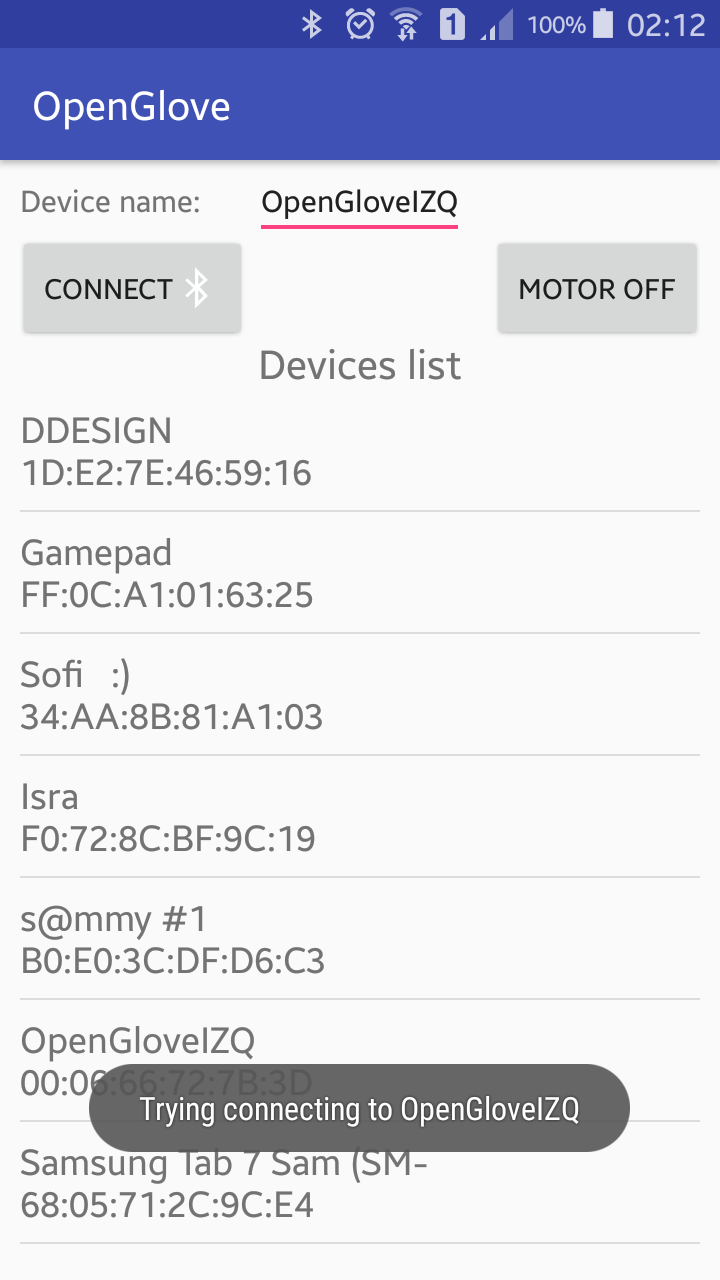
\includegraphics[width=0.3\textwidth]{images/chapter03/01-prototype.png} 
    \caption[Primer prototipo: activación de motores]{Primer prototipo: Activación de motores \\ Fuente: elaboración propia (2018).}
    \label{fig:prototype-01}
\end{figure}

Para lograr el objetivo propuesto, luego obtener los dispositivos vinculados y de la conexión con el guante mediante las APIs de bluetooth de Android, se procedió a enviar mensajes bajo el protocolo establecido en el desarrollo de Monsalve (2015). Dicho de una manera más detallada se utilizó la clase \textit{Message Generator} de la API de bajo nivel y la implementación nativa en Android para la escritura serial por medio de bluetooth. La Figura \ref{fig:prototype-01} consiste en el primer prototipo que muestra el listado de los dispositivos vinculados, la posibilidad de la conexión con el dispositivo deseado, permitiendo finalmente activar y desactivar el motor seleccionado para las pruebas. Para administrar la conexión entre los dispositivos, se requiere de un hilo\footnote{Hilo o Thread: En palabras muy resumidas, un hilo es una secuencia instrucciones dentro de un programa que se puede ejecutar independientemente de otro código, permitiendo así la ejecución en paralelo de instrucciones.} encargado de ello (\textit{ConnectedThread}), el cual se comunica con el hilo de la \textit{interfaz de usuario} (UI desde ahora)  mediante mensajes. El uso de hilos, permite administrar multiples conexiones con dispositivos Bluetooh de manera simultánea. En conclusión es posible realizar envio de mensajes bajo el protocolo que acepta OpenGlove desde una aplicación Android nativa en Java.



\subsection{Segundo prototipo: Obtención de datos desde los flexores}
\label{segundo-prototipo}
En el segundo prototipo se mantiene lo desarrollado previamente, añadiendo en esta iteración el soporte para los flexores. En este caso es necesaria la lectura desde el dispositivo OpenGlove. En la Tabla \ref{table:prototype-02} se muestra el resumen del prototipo ya mencionado. El RNF004 es cubierto parcialmente, debido a que se consulta continuamente el valor del flexor mediante funciones de bajo nivel, aumentando la latencia debido a las continuas consultas. No se presentan problemas de latencia para la activación y desactivación de motores.


%\caption[Segundo prototipo]{Segundo prototipo \\ Fuente: elaboración propia (2018).}
%\label{table:prototype-02}

\begin{table}[H]
\caption[Segundo prototipo: obtención de datos desde flexores]{Segundo prototipo\\ Fuente: elaboración propia (2018).}
\label{table:prototype-02}
\begin{tabular}{|l|l|}
\hline
\textbf{ID del prototipo} & \textbf{P002}                                                                                                                                                                                                                                                       \\ \hline
Nombre                    & Obtención de datos desde los flexores.                                                                                                                                                                                                                              \\ \hline
Objetivos                 & \begin{tabular}[c]{@{}l@{}}Verificar la correcta obtención de datos desde los flexores en \\ la aplicación de Android nativo, utilizando las APIs de bajo \\ nivel disponibles.\end{tabular}                                                                        \\ \hline
Descripción               & \begin{tabular}[c]{@{}l@{}}El segundo prototipo desarrollado agrega los métodos disponibles \\ de los flexores de la API de bajo nivel C\# hecha por Cerda (2017). \\ De esta manera, se obtiene un prototipo capaz de obtener los datos\\ del flexor.\end{tabular} \\ \hline
Requisitos funcionales    & RF001                                                                                                                                                                                                                                                              \\ \hline
Requisitos no funcionales & RNF002, RNF004 (parcialmente)
 \\ \hline
\end{tabular}
\end{table}


\begin{figure}[H]
	\centering
	\captionsetup{justification=centering}
   	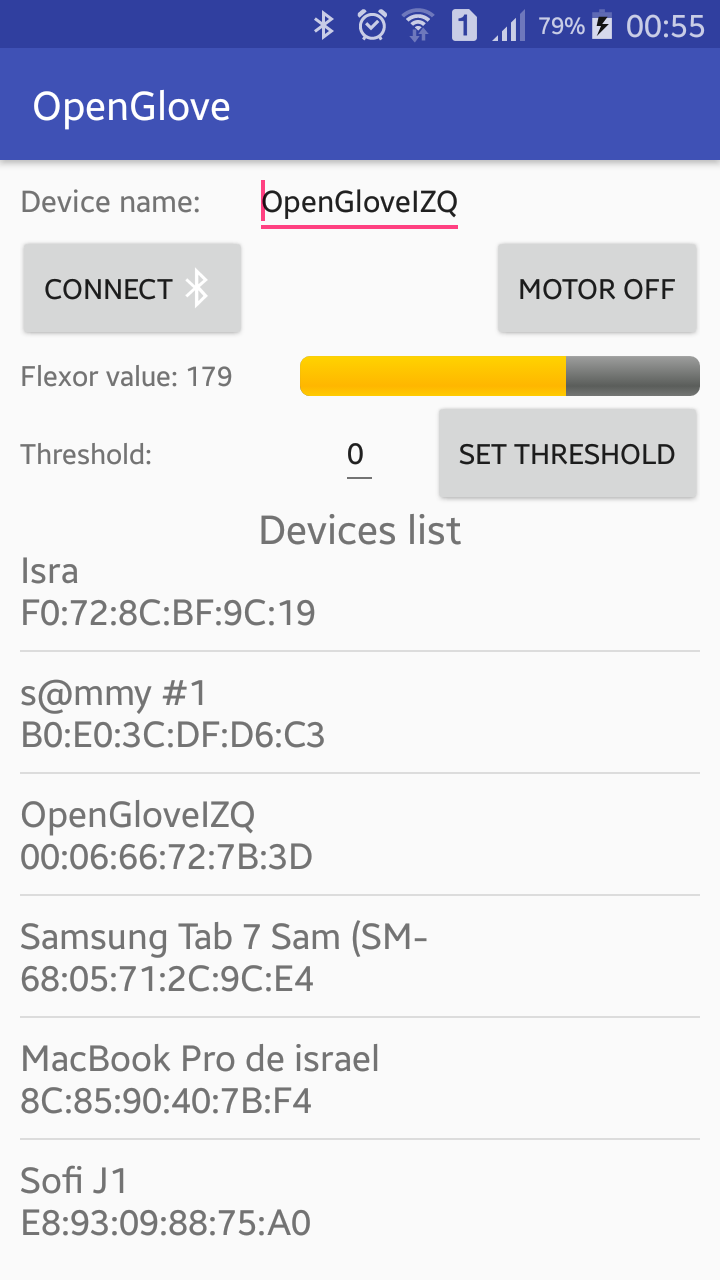
\includegraphics[width=0.3\textwidth]{images/chapter03/02-prototype.png} 
        \caption[Segundo prototipo: obtención de datos desde flexores]{Segundo prototipo: obtención de datos desde flexores \\ Fuente: elaboración propia (2018).}
    \label{fig:prototype-02}
\end{figure}

Para realizar la captura de datos del flexor, se obtiene valor actual del pin al cual el está conectado, esto se logra con el desarrollo de la función analogRead(pin) en Java basada en la API C\# de bajo nivel Cerda (2017). El hilo encargado de la administrar conexión (\textit{ConnectedThread}), tiene la responsabilidad de leer los mensajes desde OpenGlove y actualiza la UI enviando como un mensaje ente hilos el valor obtenido del flexor. Además se agregan las demás funciones de generación de mensajes relacionadas a los flexores en la API C\# ya mencionada. En la figura \ref{fig:prototype-02} se puede ver el estado actual del flexor el cual varia en un rango de entre 60 a 300 y 170 el valor medio del flexor sin aplicar fuerza.

\subsection{Tercer prototipo: Activación de motores y obtención de datos desde los flexores }
\label{tercer-prototipo}
% Xamarin C# prototype for cross platform use
En el segundo prototipo fue posible la activación del motor y obtener la información del flexor, permitiendo así comprobar la factibilidad de un desarrollo nativo en Android. En este tercer prototipo, se buscó dar soporte multiplataforma al proyecto, considerando la importancia de mantener umbrales de latencia, se optó por Xamarin. En concreto Xamarin.Forms,  que es una tecnología de desarrollo móvil multiplataforma \footnote{Traducción libre}, el cual permite desarrollar aplicaciones nativas para Android e iOS en C\#. La tabla \ref{table:prototype-03} muestra el resumen del tercer prototipo. El RNF004 es cubierto parcialmente, debido a que se consulta continuamente el valor del flexor al igual que el segundo prototipo. De igual manera no se presentan problemas de latencia para la activación y desactivación de motores.


%\caption[Tercer prototipo: activación de motores y obtención de datos desde flexores]{Tercer prototipo \\ Fuente: elaboración propia (2018).}
%\label{table:prototype-03}

\begin{table}[H]
\centering
\captionsetup{justification=centering}
\caption[Tercer prototipo: activación de motores y obtención de datos desde flexores]{Tercer prototipo \\ Fuente: elaboración propia (2018).}
\label{table:prototype-03}
\begin{tabular}{|l|l|}
\hline
\textbf{ID del prototipo} & \textbf{P003}                                                                                                                                                                                                                                                       \\ \hline
Nombre                    & Activación de motores y obtención de datos desde los flexores.                                                                                                                                                                                                                              \\ \hline
Objetivos                 & \begin{tabular}[c]{@{}l@{}}Verificar la correcta activación de motores y la obtención de \\ datos desde los flexores en la aplicación de Android nativo \\ con Xamarin.Forms, utilizando las APIs C\# de bajo nivel disponibles.\end{tabular}                                                                        \\ \hline
Descripción               & \begin{tabular}[c]{@{}l@{}}El tercer prototipo desarrollado agrega las mismas funcionalidades \\ que en el segundo prototipo.  De esta manera, se obtiene un prototipo \\ capaz de obtener los datos del flexor.\end{tabular} \\ \hline
Requisitos funcionales    & RF001                                                                                                                                                                                                                                                              \\ \hline
Requisitos no funcionales & RNF001, RNF002, RNF004 (parcialmente)                                                                                                                                                                                                                                                             \\ \hline
\end{tabular}
\end{table}



La figura \ref{fig:prototype-03} muestra el prototipo hecho en Xamarin.Forms, el cual es similar al segundo prototipo, con la diferencia en la forma de conectarse a un dispositivo bluetooth, el cual difiere en la forma de conectarse, este prototipo requiere presionar el dispositivo y aceptar el mensaje que explica el intento de conexión.


\begin{figure}[H]
	\centering
	\captionsetup{justification=centering}
   	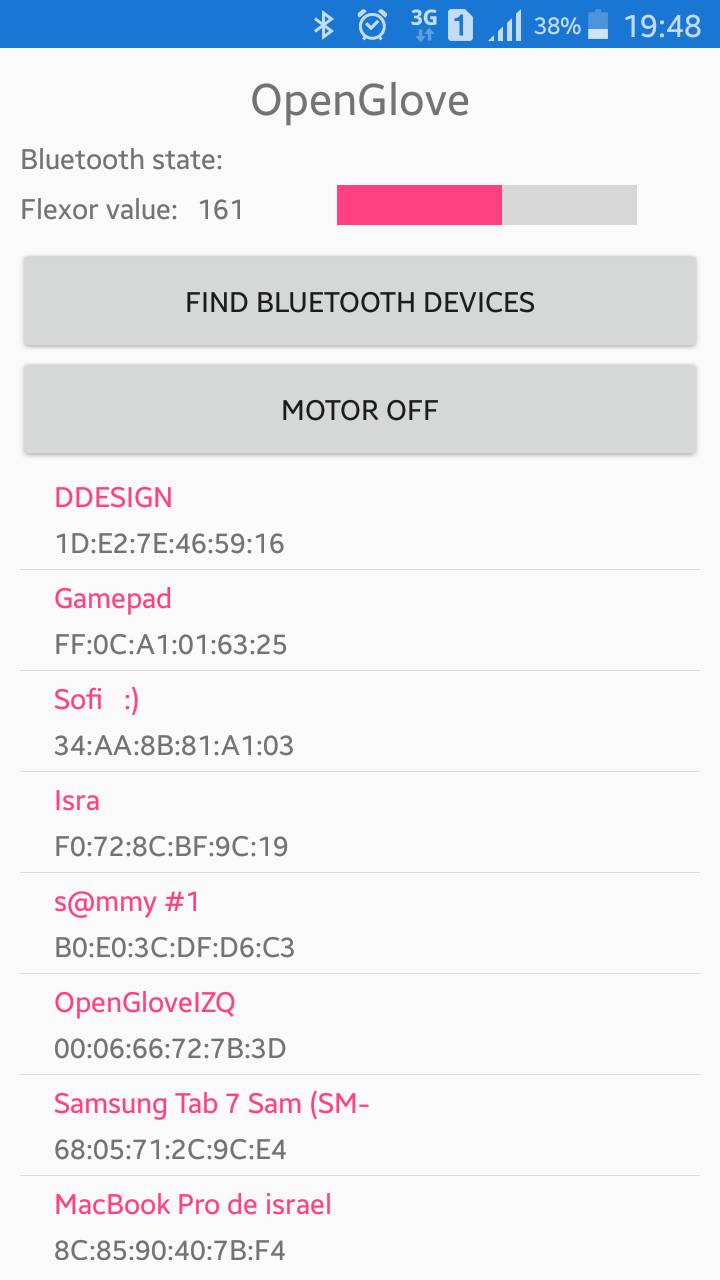
\includegraphics[width=0.3\textwidth]{images/chapter03/03-prototype.png} 
            \caption[Tercer prototipo: activación de motores y obtención de datos desde flexores]{Tercer prototipo: activación de motores y obtención de datos desde flexores \\ Fuente: elaboración propia (2018).}
    \label{fig:prototype-03}
\end{figure}





\subsection{Cuarto prototipo: Navegación aplicación, administración dispositivos Bluetooth, servidor WebSocket y configuración de la placa}
\label{cuarto-prototipo}
Este prototipo tiene como propósito cubrir los diferentes requisitos funcionales relacionados al comportamiento de la aplicación y ser la base de las siguientes iteraciones para dar soporte a los sensores de flexibilidad, actuadores e IMU. Se establece la navegación que posee la aplicación para hacer uso de todas las funcionalidades, por medio del diseño de un prototipo usando la herramienta AdobeXD en su versión grauita, con el cual se diseña, prototipa y se generan las diferentes imágenes e íconos que se utilizaron en el desarrollo del cuarto, quinto y sexto prototipo. La Figura \ref{fig:prototype-04}, muestra el prototipo desarrollado en Xamarin.Forms para Android y iOS, los cuales comparten la interfaz de usuario diferenciándose en la representaciones nativas de los elementos de cada plataforma. La Tabla \ref{table:prototype-04} muestra el resumen del prototipo ya mencionado.


%\caption[Cuarto prototipo]{Cuarto prototipo \\Fuente: elaboración propia (2018) }
%\label{table:prototype-04}

\begin{table}[H]
\caption[Cuarto prototipo]{Cuarto prototipo \\Fuente: elaboración propia (2018) }
\label{table:prototype-04}
\begin{tabular}{|l|l|}
\hline
\textbf{ID del prototipo} & \textbf{P004} \\ \hline
Nombre & \begin{tabular}[c]{@{}l@{}}Navegación aplicación, administración dispositivos Bluetooth, \\ servidor WebSocket y configuración de la placa.\end{tabular} \\ \hline
Objetivos & \begin{tabular}[c]{@{}l@{}}- Desarrollar Navegación de la aplicación (soporte iOS y Android).\\ - Desarrollar Administración de dispositivos Bluetooth.\\ - Desarrollar Administración del servidor WebSocket.\\ - Desarrollar la Configuración de la placa.\end{tabular} \\ \hline
Descripción & \begin{tabular}[c]{@{}l@{}}Este cuarto prototipo abarca los diferentes requisitos\\ funcionales relacionados al comportamiento de la aplicación y\\ de implementaciones de tecnología como el servidor WebSocket\\  embebido en la aplicación.\end{tabular} \\ \hline
Requisitos funcionales & RF001, RF002, RF003, RF004, RF008, RF010 \\ \hline
Requisitos no funcionales & RNF001, RNF002, RNF004 \\ \hline
\end{tabular}
\end{table}




\begin{figure}[H]
	\centering
	\captionsetup{justification=centering}
   	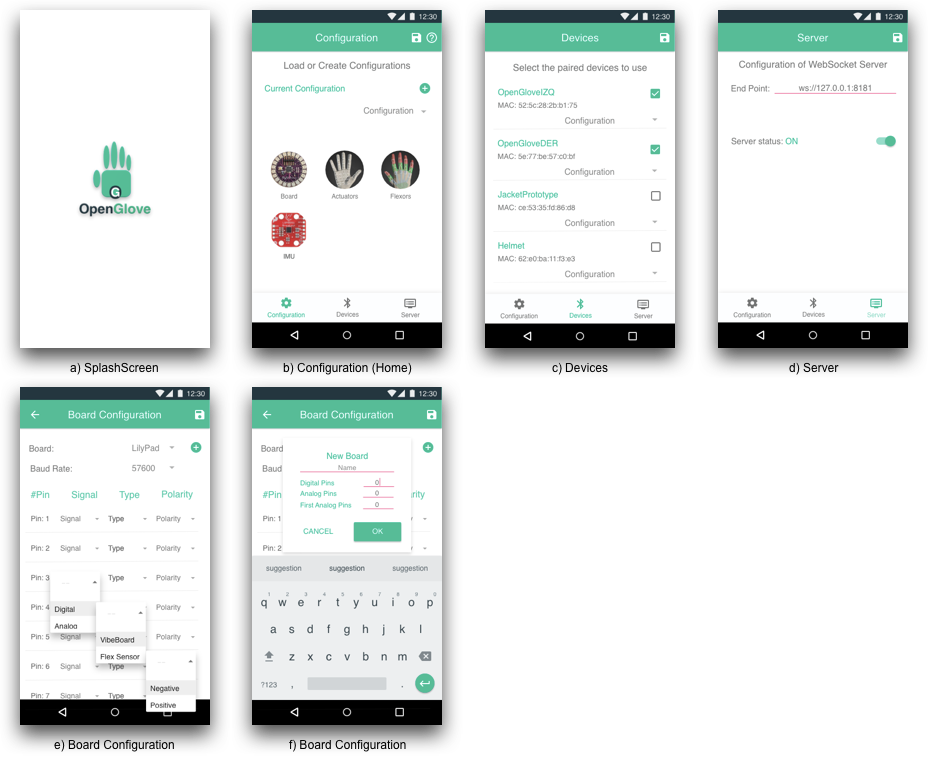
\includegraphics[width=1.0\textwidth]{images/chapter03/04-prototype/04-prototype.png} 
            \caption[Cuarto prototipo: app navigation, devices, server and board configuration]{Cuarto prototipo: app navigation, devices, server and board configuration \\ Fuente: elaboración propia (2018).}
    \label{fig:prototype-04}
\end{figure}

A continuación se describen las pantallas desarrolladas, especificando el alcance de las mismas para iOS y Android.

\begin{itemize}

\item La Figura \ref{fig:prototype-04}.a muestra el SplashScreen de la aplicación, el cual se muestra mientras se inicia la aplicación. \textbf{[Soporte completo: iOS y Android]}

\item La Figura \ref{fig:prototype-04}.b muestra el menú principal de la aplicación de configuración, en el cual es posible cargar configuraciones existentes o bien crear una nueva configuración, la cual contiene la configuración de la placa, de los actuadores, de los flexores y del sensor IMU. Esta aplicación seleccionada o creada puede ser modificada del menú principal accediendo a las pantallas que permiten configurar la placa, actuadores, flexores e IMU. La aplicación posee una navegación basada en BottomNavigation, la cual corresponde a una	 barra de navegación inferior que permite acceder al menú de configuración general, la configuración de dispositivos Bluetooth y la configuración del servidor. \textbf{[Soporte completo: iOS y Android]}

\item La Figura \ref{fig:prototype-04}.c muestra una lista con los dispositivos Bluetooth emparejados, permitiendo ver el nombre y dirección MAC de ellos. También permite elegir los dispositivos Bluetooth que se utilizarán junto la configuración que se le desee aplicar. La aplicación en iOS no puede mostrar la lista de dispositivos emparejados, no se implementó la clase Communication para el proyecto iOS, porque está fuera del alcance de este trabajo \textbf{[Soporte completo: Android]}.

\item La Figura \ref{fig:prototype-04}.d muestra la pantalla referente al servidor WebSocket, permitiendo definir la dirección de acceso al servidor y el encendido y apagado del mismo. Para la implementación del servidor WebSocket se utilizó el paquete de software Fleck, el que se encuentra disponible en la plataforma NuGet \footnote{Paquetes de software NuGet https://www.nuget.org/packages} junto a otros paquetes que pueden ser utilizados si son compatibles con la versión .NET standar 2.0. Con este paquete se desarrolló la clase OpenGloveServer para su uso en la aplicación de configuración. En esa clase se instancia un servidor y  donde se establecen los EventHandler necesarios para mandar mensajes entre los hilos que administran las conexiones de sus dispositivos Bluetooth (clase Communication) y el servidor WebSocket (clase OpenGloveServer) \textbf{[Soporte completo: iOS y Android]}.

\item La Figura \ref{fig:prototype-04}.e muestra la pantalla que permite definir la configuración de la placa, creando una nueva placa o utilizando alguna previamente creada, como puede ser la placa LilyPad utilizada en este trabajo. En esta pantalla de la aplicación, se puede elegir o crear una placa y seleccionar el BaudRate \footnote{El baud rate especifica la velocidad en la que se envían los datos por una línea serial, usualmente son expresadas en unidades de bits por segundo (bps). \url{https://learn.sparkfun.com/tutorials/serial-communication/rules-of-serial}
} con el que se trabajará. Luego de ello se procede a configurar los pines de placa considerando la configuración física de los mismos, definiendo el tipo de señal, pines digitales y análogos, si el pin corresponde a flexor o un actuador e indicando su polaridad, positiva o negativa \textbf{[Soporte completo: iOS y Android]}.

\item La Figura \ref{fig:prototype-04}.f muestra el diálogo utilizado para crear una nueva configuración de placa, pidiendo el nombre de la placa, el pin donde comienzan los pines análogos (depende de la placa específica \citep{tesis-cerda-rodrigo}), cantidad de pines digitales y análogos \textbf{[Soporte completo: iOS y Android]}.

\end{itemize}






\subsection{Quinto  prototipo: Mapeo de actuadores y prueba de actuadores}
\label{quinto-prototipo}
Este prototipo tiene como propósito cubrir los diferentes requisitos funcionales relacionados a los actuadores.  La Tabla \ref{table:prototype-05} muestra el resumen del prototipo antes mencionado. Este prototipo utilizó como base el cuarto prototipo desarrollado.

%\caption[Quinto prototipo]{Quinto prototipo \\Fuente: elaboración propia (2018)}
%\label{table:prototype-05}

\begin{table}[H]
\caption[Quinto prototipo]{Quinto prototipo \\Fuente: elaboración propia (2018)}
\label{table:prototype-05}
\begin{tabular}{|l|l|}
\hline
\textbf{ID del prototipo} & \textbf{P005}                                                                                                                                                                                     \\ \hline
Nombre                    & Mapeo de actuadores y prueba de actuadores                                                                                                                                                        \\ \hline
Objetivos                 & \begin{tabular}[c]{@{}l@{}}- Desarrollar el mapeo actuador-region\\ - Desarrollar la prueba de actuadores\end{tabular}                                                                            \\ \hline
Descripción               & \begin{tabular}[c]{@{}l@{}}Este quinto prototipo abarca los diferentes requisitos\\ funcionales relacionados a los actuadores, sumándose\\ a lo desarrollado en el cuarto prototipo.\end{tabular} \\ \hline
Requisitos funcionales    & \begin{tabular}[c]{@{}l@{}}RF001, RF002, RF003, RF004, RF005, RF006, RF007,\\ RF008, RF009, RF010, RF011\end{tabular}                                                                             \\ \hline
Requisitos no funcionales & RNF001, RNF002, RNF004                                                                                                                                                                            \\ \hline
\end{tabular}
\end{table}

\begin{figure}[H]
	\centering
	\captionsetup{justification=centering}
   	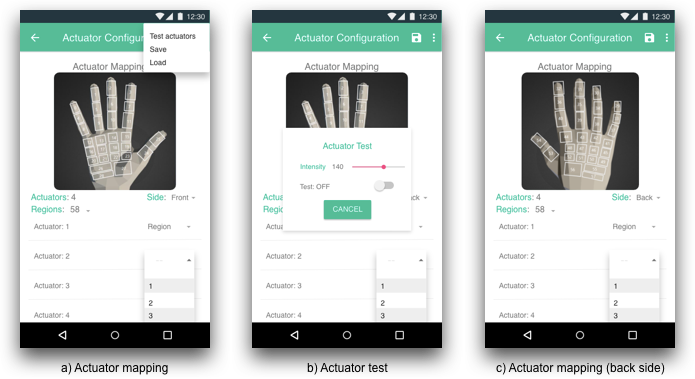
\includegraphics[width=1.0\textwidth]{images/chapter03/05-prototype/05-prototype.png} 
            \caption[Quinto prototipo: actuator mapping and  actuator test]{Quinto prototipo: actuator mapping and actuator test \\ Fuente: elaboración propia (2018).}
    \label{fig:prototype-05}
\end{figure}

En paralelo al desarrollo de este prototipo fue necesario el desarrollo de la API C\#, es decir el desarrollo de un cliente WebSocket utilizando el paquete de software WebSocketSharp\footnote{WebSocketSharp: \url{https://www.nuget.org/packages/WebSocketSharp/1.0.3-rc11}}. El cliente es quien envía mensajes al servidor que está dentro de la aplicación de configuración, para activar los actuadores deseados. Para ello se incluyen métodos para la activación de motores, en el cual se especifica el dispositivo Bluetooth y una lista de regiones a activar, las cuales son traducidas a los mensajes generados por la API de bajo nivel de OpenGlove.

A continuación se describen las pantallas desarrolladas, especificando el alcance de las mismas para iOS y Android.

\begin{itemize}

\item La Figura \ref{fig:prototype-05}.a muestra la pantalla que permite el mapeo actuador-región, mostrando una lista de los actuadores identificados desde la configuración de la placa. Es posible cambiar la imagen que representa el mapeo del dispositivo Bluetooth, para ello se requiere definir la cantidad de regiones que posee el lado frontal y trasero al momento de definir la cantidad de regiones, especificando también el número inicial que identifica a las regiones (iniciando en 1 o en 0 por ejemplo). El mapeo se realiza seleccionando la región desde una lista desplegable en cada actuador, la cual es generada dependiendo de la configuración inicial de la cantidad de regiones. \textbf{[Soporte completo: iOS y Android]}.

\item La Figura \ref{fig:prototype-05}.b muestra el diálogo que permite realizar las pruebas de los actuadores mapeados, permitiendo iniciar y detener la prueba con la intensidad seleccionada. La prueba se termina una vez se cierra el diálogo o se desactiva dentro del diálogo. La aplicación en iOS no puede activar regiones mapeadas, porque no se implementó la clase Communication para el proyecto iOS, porque está fuera del alcance de este trabajo \textbf{[Soporte completo: Android]}.

\item La Figura \ref{fig:prototype-05}.c muestra el segundo lado de la imagen de mapeo de actuadores, de la pantalla de mapeo mostrada en la Figura \ref{fig:prototype-05}.a.

\end{itemize}




\subsection{Sexto  prototipo: Mapeo de flexores, prueba de flexores y la configuración del IMU.}
\label{sexto-prototipo}
Este prototipo tiene como propósito cubrir los diferentes requisitos funcionales relacionados a los flexores e IMU. Se utilizó como base el quinto prototipo ya descrito. 

Este prototipo tiene como propósito cubrir los diferentes requisitos funcionales relacionados a los flexores e IMU.  La Tabla \ref{table:prototype-06} muestra el resumen del prototipo antes mencionado. Este prototipo utilizó como base el quinto prototipo desarrollado.

%\caption[Sexto prototipo]{Sexto prototipo \\Fuente: elaboración propia (2018)}
%\label{table:prototype-06}

\begin{table}[H]
\caption[Sexto prototipo]{Sexto prototipo \\Fuente: elaboración propia (2018)}
\label{table:prototype-06}
\begin{tabular}{|l|l|}
\hline
\textbf{ID del prototipo} & \textbf{P006}                                                                                                                                                                                                                                                                                                             \\ \hline
Nombre                    & \begin{tabular}[c]{@{}l@{}}Mapeo de flexores, prueba de flexores y la configuración\\ del IMU.\end{tabular}                                                                                                                                                                                                               \\ \hline
Objetivos                 & \begin{tabular}[c]{@{}l@{}}- Desarrollar el mapeo flexor-region\\ - Desarrollar la prueba de flexores\\ - Desarrollar la configuración del IMU\end{tabular}                                                                                                                                                               \\ \hline
Descripción               & \begin{tabular}[c]{@{}l@{}}Este sexto prototipo abarca los diferentes requisitos\\ funcionales relacionados a los flexores e IMU, sumándose\\ a lo desarrollado en el quinto prototipo. Esto es posible\\ gracias al desarrollo de la API C\#, la cual es replicada para\\ el lenguaje de programación Java.\end{tabular} \\ \hline
Requisitos funcionales    & \begin{tabular}[c]{@{}l@{}}RF001, RF002, RF003, RF004, RF005, RF006, RF007,\\ RF008, RF009, RF010, RF011, RF012, RF013, RF014,\\ RF015, RF016, RF018, RF019, RF020, RF021, RF022,\\ RF023\end{tabular}                                                                                                                    \\ \hline
Requisitos no funcionales & RNF001, RNF002, RNF003, RNF004, RNF005, RNF006                                                                                                                                                                                                                                                                            \\ \hline
\end{tabular}
\end{table}


\begin{figure}[H]
	\centering
	\captionsetup{justification=centering}
   	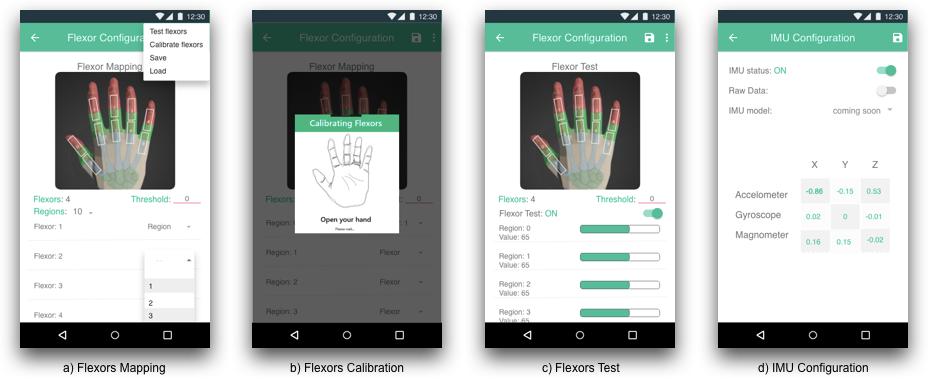
\includegraphics[width=1.0\textwidth]{images/chapter03/06-prototype/06-prototype.png} 
            \caption[Sexto prototipo: flexor mapping, flexor test and IMU configuration]{Sexto prototipo: flexor mapping, flexor test and IMU configuration\\ Fuente: elaboración propia (2018).}
    \label{fig:prototype-06}
\end{figure}

De igual manera al quinto prototipo, se agregan métodos que permiten el desarrollar las funcionalidades referentes a los flexores e IMU, permitiendo definir el Threshold (límite en que, se enviará un dato de un flexor si la diferencia es mayor o igual a este valor), agregar o remover flexores de una región, calibrar los flexores y confirmar la calibración. También permite iniciar o detener el IMU y definir si recibir datos crudos o procesados.

A continuación se describen las pantallas desarrolladas, especificando el alcance de las mismas para iOS y Android.

\begin{itemize}

\item La Figura \ref{fig:prototype-06}.a muestra la pantalla de mapeo flexor-region de igual manera que el de actuadores, agregando la asignación del Threshold que se utilizará cuando en la prueba de flexores y cuando se le asigne la configuración al o los dispositivos Bluetooth. \textbf{[Soporte completo: iOS y Android]}.

\item La Figura \ref{fig:prototype-06}.b muestra una pantalla sobrepuesta con una animación, la cual indica que es necesario mover las articulaciones para calibrar los flexores. La aplicación en iOS no puede calibrar los flexores, porque no se implementó la clase Communication para el proyecto iOS, porque está fuera del alcance de este trabajo \textbf{[Soporte completo: Android]}.

\item La Figura \ref{fig:prototype-06}.c muestra la pantalla que permite probar los flexores previamente mapeados, también se puede definir el Threshold antes de activar o desactivar la prueba de los flexores. La aplicación en iOS no puede obtener datos de los flexores, porque no se implementó la clase Communication para el proyecto iOS, porque está fuera del alcance de este trabajo \textbf{[Soporte completo: Android]}.

\item La Figura \ref{fig:prototype-06}.d muestra la pantalla de configuración del sensor de rastreo IMU, en la cual se puede iniciar o detener el mismo, configurar el envío de datos crudos o procesados. También permite ver los datos recibidos por el acelerómetro, giroscopio y magnetómetro para los ejes $X$, $Y$ y $Z$.Agregar soporte a otros modelos de sensores de rastreo IMU. No es posible seleccionar otro modelo de IMU aparte de SparkFun LSM9DS1, dado que requiere bibliotecas de software específicas en el código de la placa Arduino. Podría definirse que la selección de modelo de placa IMU, permita cargar código en la placa Arduino, incluyendo a las librerías y código específico del modelo del IMU. Esto podría ser realizado utilizando la conexión Bluetooth o por medio de conexión USB adecuada. Por ejemplo, la herramienta Bluino Loader - Arduino IDE\footnote{Bluino Loader: https://www.hackster.io/mansurkamsur/upload-sketch-arduino-over-bluetooth-using-android-f1ce55} permite cargar código a la placa Arduino por Bluetooth o USB. La aplicación en iOS no puede calibrar obtener datos desde el IMU, porque no se implementó la clase Communication para el proyecto iOS, porque está fuera del alcance de este trabajo \textbf{[Soporte completo: Android]}.

\end{itemize}

	\section{APIs}
%según implementación de las APIs en cada prototipo
Para que los desarrolladores puedan hacer uso de las funcionalidades disponibles en el SDK, se requiere del soporte de distintos lenguajes de programación permitiendo abarcar a las más importantes plataformas tecnológicas de Realidad Virtual, Aumentada y Mixta. Por lo tanto se considera la interoperabilidad para los lenguajes C\# y Java, como se especificó en el Requisito no funcional RNF003. Estas APIs fueron desarrolladas paralelamente a la aplicación de configuración pues se hace uso de ella, iniciando con la API de alto nivel de C\#. Una vez que la API C\# fue completada, se replicó utilizando el lenguaje Java. Las mencionadas APIs son clientes WebSockets que establecen conexión con el Servidor WebSocket provisto y administrado por la aplicación de configuración. El primer, segundo y tercer prototipo no incluyen el desarrollo de las APIs de alto nivel, porque estos prototipos abarcaron permitieron evaluar la factibilidad de distintas tecnologías y definir el trabajo a seguir en los siguientes prototipos.

El capítulo Diseño e Implementación especifica en mayor detalle los aspectos arquitecturales  de la solución y del comportamiento en los cuales las APIs están involucradas.

\subsection{Cuarto prototipo}
Este prototipo no incluye desarrollo de la APIs de alto nivel, pero si la implementación de distintas tecnologías y la definición del protocolo de mensajes a utilizar por las APIs de los siguientes prototipos. En este prototipo se implementó un servidor WebSocket que recibe conexiones entrantes de clientes WebSocket, los cuales pueden ser la aplicación de configuración y una aplicación de VR por ejemplo. El servidor WebSocket puede activarse o desactivarse desde la aplicación de configuración, permitiendo además definir el el punto de acceso o EndPoint del Servidor. El servidor WebSocket se comunica con la API de Bajo nivel mediante el uso de EventHandlers, los cuales permiten por una parte al Servidor recibir los mensajes provenientes de los dispositivos Bluetooth (datos de flexores e IMU) como también el enviar mensajes para la activación de actuadores, obtención de lista de dispositivos vinculados y la conexión de a los mismos. Es importante destacar que la administración de la conexión de dispositivos Bluetooth está implementada para el Sistema Operativo Android, por lo que es necesario realizar la implementación específica para iOS.
	
\subsection{Quinto prototipo}
En este prototipo se  abarcan las funcionalidades referidas a los actuadores, por tanto se aplicó el protocolo de comunicación definido en el cuarto prototipo, entre los clientes y el servidor WebSocket. Con ello se logró cubrir la inicialización, activación y mapeo de los actuadores mediante la API de alto nivel en C\#. Gracias a estas funcionalidades, la aplicación de configuración permite realizar el mapeo y pruebas de activación de los actuadores de los distintos dispositivos OpenGlove conectados.

\subsection{Sexto prototipo}
Este prototipo incluye todas las funcionalidades de la API C\# para el uso de OpenGlove en dispositivos móviles utilizando este lenguaje de programación. Esto se logró desarrollando las funcionalidades que no fueron cubiertas en el quinto prototipo, las referidas a los sensores de flexibilidad e IMU. Las funcionalidades implementadas respecto a los sensores de flexibilidad , permiten agregar agregar un flexor a una región para iniciar la transmisión de datos, remover un flexor de una región, calibrar los flexores, testear los flexores asignados a una región y la asignación de un umbral o Threshold (el dispositivo OpenGlove, enviará el dato de un flexor si la diferencia es mayor o igual a este valor). Respecto a las funcionalidades referidas al IMU, se permite iniciar el IMU, asignar el status del IMU, recibir datos crudos o procesados del IMU. Inicio y suspensión de lectura de datos es una funcionalidad que involucra a ambos sensores.
	\section{Resumen}

Durante el desarrollo del SDK, fue necesario un desarrollo de seis prototipos, los primeros tres que permitieron la validando la factibilidad de un desarrollo nativo en Android comparado al desarrollo multiplataforma con Xamarin.Forms. Los siguientes prototipos corresponden al desarrollo de la aplicación de configuración y las APIs para lograr cumplir con los requisitos funcionales y no funcionales del SDK. La Tabla \ref{table:RF-summary}
muestra el resumen de los requisitos funcionales, en el cual se aprecia la cobertura de los mismos en cada prototipo anteriormente detallado. La Tabla \ref{table:RNF-summary}, muestra de la misma forma la cobertura de los requisitos no funcionales del SDK.


%\centering
%\captionsetup{justification=centering}
%\caption[Matriz de prototipos de software vs requisitos funcionales]{Matriz de prototipos de software vs requisitos funcionales \\ Fuente: Elaboración propia (2018)}
%\label{table:RF-summary}

\begin{table}[H]
\centering
\captionsetup{justification=centering}
\caption[Matriz de prototipos de software vs requisitos funcionales]{Matriz de prototipos de software vs requisitos funcionales \\ Fuente: Elaboración propia (2018)}
\label{table:RF-summary}
\begin{tabular}{|c|c|c|c|c|c|c|}
\hline
 & P001 & P002 & P003 & P004 & P005 & P006 \\ \hline
RF001 & X & X & X & X & X & X \\ \hline
RF002 &  &  &  & X & X & X \\ \hline
RF003 &  &  &  & X & X & X \\ \hline
RF004 &  &  &  & X & X & X \\ \hline
RF005 &  &  &  &  & X & X \\ \hline
RF006 &  &  &  &  & X & X \\ \hline
RF007 &  &  &  &  & X & X \\ \hline
RF008 & X & X & X & X & X & X \\ \hline
RF009 &  &  &  &  & X & X \\ \hline
RF010 &  &  &  & X & X & X \\ \hline
RF011 &  &  &  &  & X & X \\ \hline
RF012 &  &  &  &  &  & X \\ \hline
RF013 &  &  &  &  &  & X \\ \hline
RF014 &  &  &  &  &  & X \\ \hline
RF015 &  &  &  &  &  & X \\ \hline
RF016 &  &  &  &  &  & X \\ \hline
RF017 &  &  &  &  &  & X \\ \hline
RF018 &  &  &  &  &  & X \\ \hline
RF019 &  &  &  &  &  & X \\ \hline
RF020 &  &  &  &  &  & X \\ \hline
RF021 &  &  &  &  &  & X \\ \hline
RF022 &  &  &  &  &  & X \\ \hline
RF023 &  &  &  &  &  & X \\ \hline
\end{tabular}
\end{table}


%\centering
%\captionsetup{justification=centering}
%\caption[Matriz de prototipos de software vs requisitos no funcionales]{Matriz de prototipos de software vs requisitos no funcionales \\ Fuente: Elaboración propia (2018)}
%\label{table:RNF-summary}

\begin{table}[H]
\centering
\captionsetup{justification=centering}
\caption[Matriz de prototipos de software vs requisitos no funcionales]{Matriz de prototipos de software vs requisitos no funcionales \\ Fuente: Elaboración propia (2018)}
\label{table:RNF-summary}
\begin{tabular}{|c|c|c|c|c|c|c|}
\hline
 & P001 & P002 & P003 & P004 & P005 & P006 \\ \hline
RNF001 &  &  & X & X & X & X \\ \hline
RNF002 & X & X & X & X & X & X \\ \hline
RNF003 &  &  &  &  &  & X \\ \hline
RNF004 & X & X &  & X & X & X \\ \hline
\end{tabular}
\end{table}
	
%\newpage
\chapter{Diseño e implementación}
	\section{Arquitectura general}

La Figura \ref{fig:arquitectura-open-glove}, muestra la arquitectura general de OpenGlove, donde es posible ver el trabajo previo realizado por \cite{tesis-monsalve-rodrigo}, \cite{tesis-meneses-sebastian} y \cite{tesis-cerda-rodrigo}, como también el trabajo que resulta de este proyecto y el que se realizará en un futuro.

\begin{figure}[H]
  \begin{center} 
   	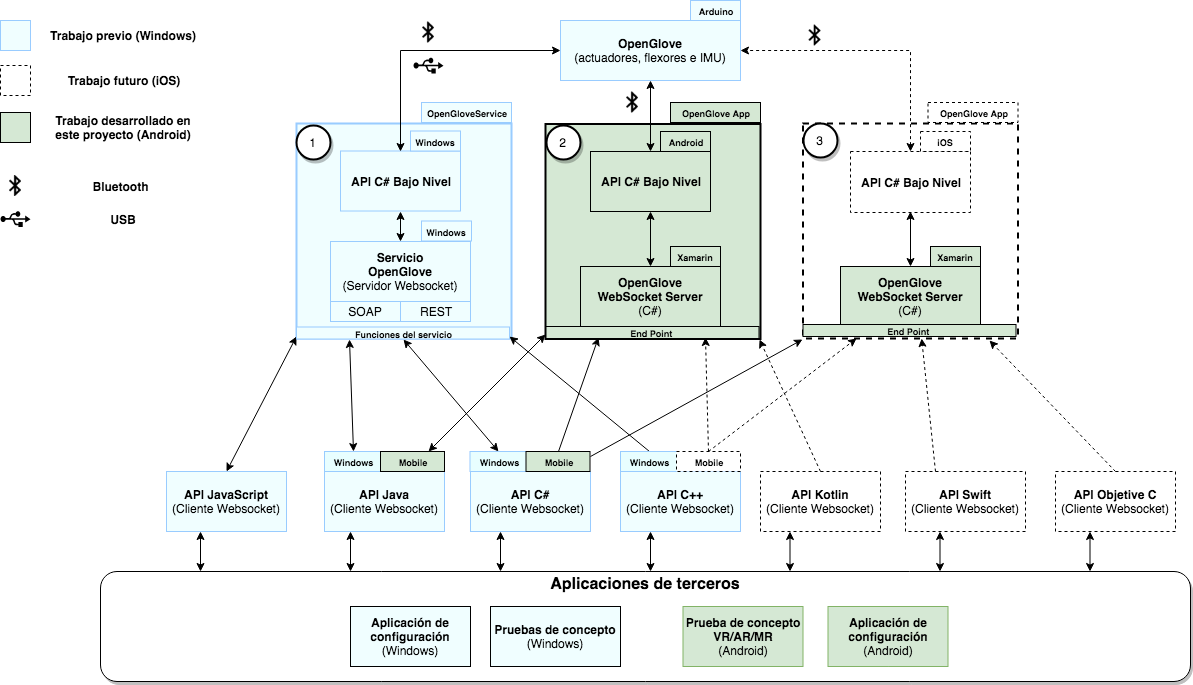
\includegraphics[width=1.0\textwidth]{images/chapter04/OpenGlove-Architecture-General.png} 
    \caption[Arquitectura de Openglove]{Arquitectura de OpenGlove \\Fuente: Elaboración propia (2018)}
    \label{fig:arquitectura-open-glove}
  \end{center}
\end{figure}

La aplicación de configuración de OpenGlove desarrollada en este proyecto, permite comunicarse con dispositivos OpenGlove a través de comunicación serial Bluetooth. Para acceder a sus funcionalidades los desarrolladores hacen uso de las APIs de alto nivel, las cuales corresponden a clientes WebSocket. Éstas pueden ser utilizadas en cualquier aplicación compatible con el lenguaje de la API a utilizar. Dado que se utiliza Xamarin.Forms para desarrollar aplicaciones nativas multiplataforma, para iOS y Android, el servidor Websocket es desarrollado utilizando bibliotecas de software de C\#, para que ambas plataformas compartan el código. La API de bajo nivel, debe ser específica en cada sistema operativo, por las diferencias de comunicación presentes en cada uno. Por esta misma razón se desarrollan las APIs de alto nivel en  Java y C\#. La primera permite hacer uso de OpenGlove en proyectos Android y la segunda permite hacer aplicaciones para iOS y Android utilizando Xamarin. El uso de Xamarin.Forms permite reutilizar código de la Interfaz de Usuario y desarrollar de manera específica para cada plataforma utilizando un mismo lenguaje de programación. Cabe destacar que la comunicación realizada entre las APIs y la aplicación es mediante WebSockets considerando que OpenGlove es una aplicación que transmite datos en tiempo real.

\begin{figure}[H]
  \begin{center} 
   	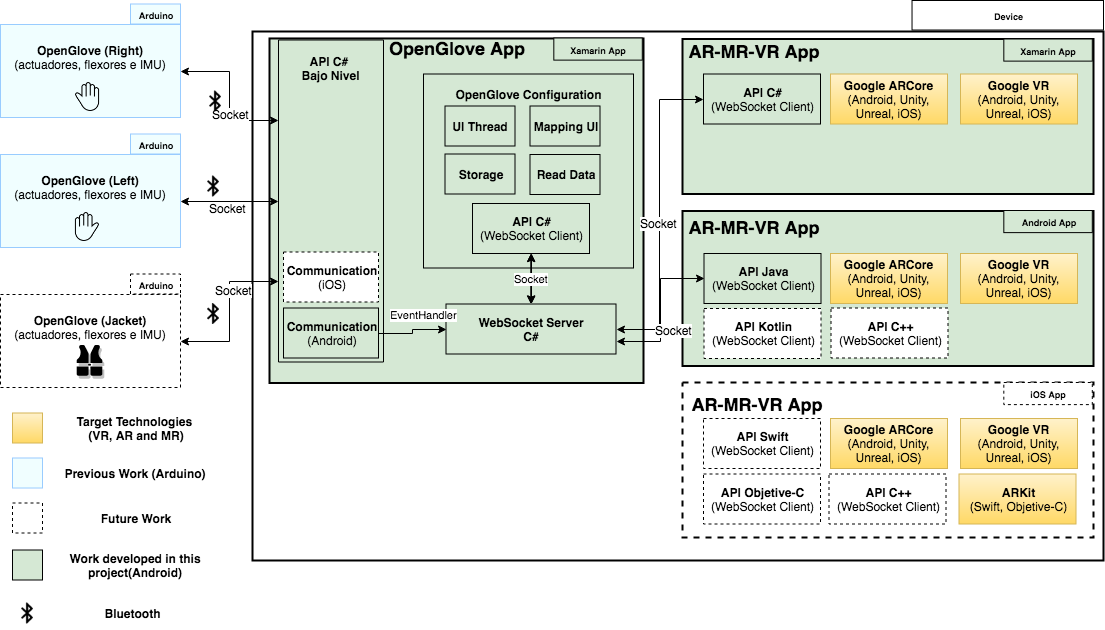
\includegraphics[width=1.0\textwidth]{images/chapter04/OpenGlove-Architecture-Specification.png} 
    \caption[Detalle Arquitectura de Openglove]{Detalle Arquitectura de OpenGlove \\Fuente: Elaboración propia (2018)}
    \label{fig:detalle-arquitectura-open-glove}
  \end{center}
\end{figure}

La Figura \ref{fig:detalle-arquitectura-open-glove} muestra el detalle de la arquitectura considerando el objetivo de uso de las APIs de alto nivel en Java y C\#. Las APIs de alto nivel mencionadas permiten el desarrollo de aplicaciones de terceros en Android nativo usando Java o con C\# utilizando Xamarin. Para realizar aplicaciones de AR o VR, se puede utilizar Google ARCore y Google VR respectivamente. Ambas herramientas de Google están disponibles para Android, iOS, Unity y Unreal.

Esta arquitectura establece al servidor WebSocket como proveedor de las funcionalidades referentes a los actuadores, flexores e IMU. Por tanto la aplicación de configuración y las aplicaciones de terceros utilizan las mismas APIs de alto nivel para su desarrollo.

Dado el alcance de la solución, no se ha desarrollado APIs de alto nivel que tengan como objetivos aplicaciones de terceros para iOS, para lo cual requiere un dispositivo iPhone real para realizar las pruebas de Bluetooth y WebSockets, o en su defecto un MacBook para poder visualizar la interfaz de la aplicación, pero sin hacer uso de las funcionalidades Bluetooth ni WebSocket. También es importante recalcar la necesidad de implementar parte de la API de bajo nivel en C\# ( Communication ) específica para iOS para gestionar las conexiones de los dispositivos Bluetooth y la administración de mensajes entre la API de bajo nivel y el servidor WebSocket. Este es un trabajo que se puede realizar a futuro para dar soporte a OpenGlove en iOS.



	\section{Estructura}
En esta sección se detalla la estructura de los distintos componentes de sofware desarrollados, los cuales son: el servicio que expone las funcionalides, las APIs que las consumen, el software de configuración  y el diagrama de clases de cada uno.

\subsection{Servicio}
\subsection{APIs}
\subsection{Software de configuración}
	\section{Comportamiento}
\label{seccion-comportamiento-apis}
Para comprender el comportamiento de las APIs de alto nivel, es necesario complementar lo detallado sobre la clase OpenGlove en la Subsección \ref{subseccion-estructura-apis-hl}, en la cual se habló sobre la estructura de las mismas. Cada instancia de la clase OpenGlove de alto nivel, permite ejecutar acciones sobre su cliente WebSocket, el servidor WebSocket al que se conecta, a las configuraciones de su instancia de la clase OpenGloveDevice alojada en el servidor y realizar acciones sobre el software de control Arduino. Además, cada instancia provee un fácil consumo de los datos provenientes de Arduino. La suma de esto es lo que hace posible una representación de los dispositivos OpenGlove en las APIs de alto nivel en tiempo real, incluyendo el envío de mensajes de manera bidireccional y full-duplex para los lenguajes de programación C\# y Java. Con esto se facilita que otras APIs de alto nivel pueden ser desarrolladas, utilizando lenguajes de programación que permitan: el manejo de eventos o funciones lambda o el envío de mensajes entre hilos, además del uso de Clientes WebSocket (API WebSocket y protocolo RFC 6455). De esta forma, se reduce la necesidad de agregar lógica compleja en la API de alto nivel.

A continuación se describe el comportamiento general de los métodos disponibles en las APIs de alto nivel, utilizando diagramas de actividades. Se agruparon estos métodos según su nivel de interacción con las diferentes capas de abstracción del SDK. Las capas de abstracción corresponden a: la API de alto nivel (Cliente WebSocket), el Servidor WebSocket, las instancias de la clase OpenGloveDevice, las instancias de LegacyOpenGlove (API C\# de bajo nivel) y el software de control Arduino.



\subsection{Métodos aplicados sobre cliente WebSocket}
\label{subsection:method-websocket-client}

Los métodos que pueden ser aplicados sobre el cliente WebSocket se muestran en la Figura \ref{fig:methods-0-api-hl}. Estos métodos son ejecutados por la aplicación que utiliza una instancia de OpenGlove, realizando la acción sobre el cliente WebSocket. Esto se detalla en el diagrama de actividades de la Figura \ref{fig:activity-diagrams-0-api-hl}. Adicionalmente, en el caso que se logre la conexión con el servidor WebSocket, el evento OnOpen del cliente es invocado. Cuando se invoca ese evento, se agrega la instancia OpenGlove al servidor  y se inicia la captura de datos. Eso se realizó utilizando los métodos AddOpenGloveDeviceToServer y StartCaptureDataFromServer respectivamente. El comportamiento de estos dos métodos mencionados se incluyen en la Subsección \ref{subsection:method-websocket-server}.

\begin{figure}[H]
  \begin{center} 
      \begin{lstlisting}
	// OpenGloveActions: OpenGlove High level API (WebSocketClient)
	public void ConnectToWebSocketServer();
	public void DisconnectFromWebSocketServer();
	\end{lstlisting}
   \captionsetup{justification=centering}
    \caption[Métodos aplicados sobre el cliente WebSocket]{Métodos aplicados sobre el cliente WebSocket \\Fuente: Elaboración propia (2018)}
    \label{fig:methods-0-api-hl}
  \end{center}
\end{figure}



\begin{figure}[H]
  \begin{center} 
   	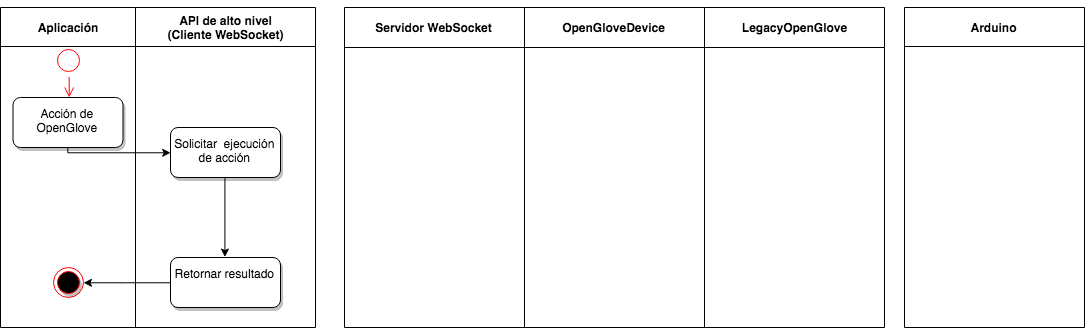
\includegraphics[width=1.0\textwidth]{images/chapter04/ActivityDiagrams-OpenGloveActions-0.png} 
   	\captionsetup{justification=centering}
    \caption[Diagrama de actividades de los métodos aplicados sobre el cliente WebSocket]{Diagrama de actividades de los métodos aplicados sobre el cliente WebSocket\\Fuente: Elaboración propia (2018)}
    \label{fig:activity-diagrams-0-api-hl}
  \end{center}
\end{figure}




\subsection{Métodos aplicados sobre servidor WebSocket}
\label{subsection:method-websocket-server}
Los métodos que pueden ser aplicados sobre el servidor WebSocket se muestran en la Figura \ref{fig:methods-1-websocket-server}. Estos métodos son ejecutados por la aplicación que utiliza una instancia de OpenGlove, realizando la acción sobre el servidor WebSocket, pasando por la capa intermedia del cliente WebSocket. El comportamiento de estos métodos se aprecia en el diagrama de actividades de la Figura \ref{fig:activity-diagrams-1-websocket-server}.




\begin{figure}[H]
  \begin{center} 
\begin{lstlisting}
// OpenGloveActions: WebSocket Server
public void AddOpenGloveDeviceToServer();
public void RemoveOpenGloveDeviceFromServer();
public void SaveOpenGloveConfiguration();
public void StartCaptureDataFromServer();
public void StopCaptureDataFromServer();
\end{lstlisting}
   \captionsetup{justification=centering}
    \caption[Métodos aplicados sobre el servidor WebSocket]{Métodos aplicados sobre el servidor WebSocket \\Fuente: Elaboración propia (2018)}
    \label{fig:methods-1-websocket-server}
  \end{center}
\end{figure}


\begin{figure}[H]
  \begin{center} 
   	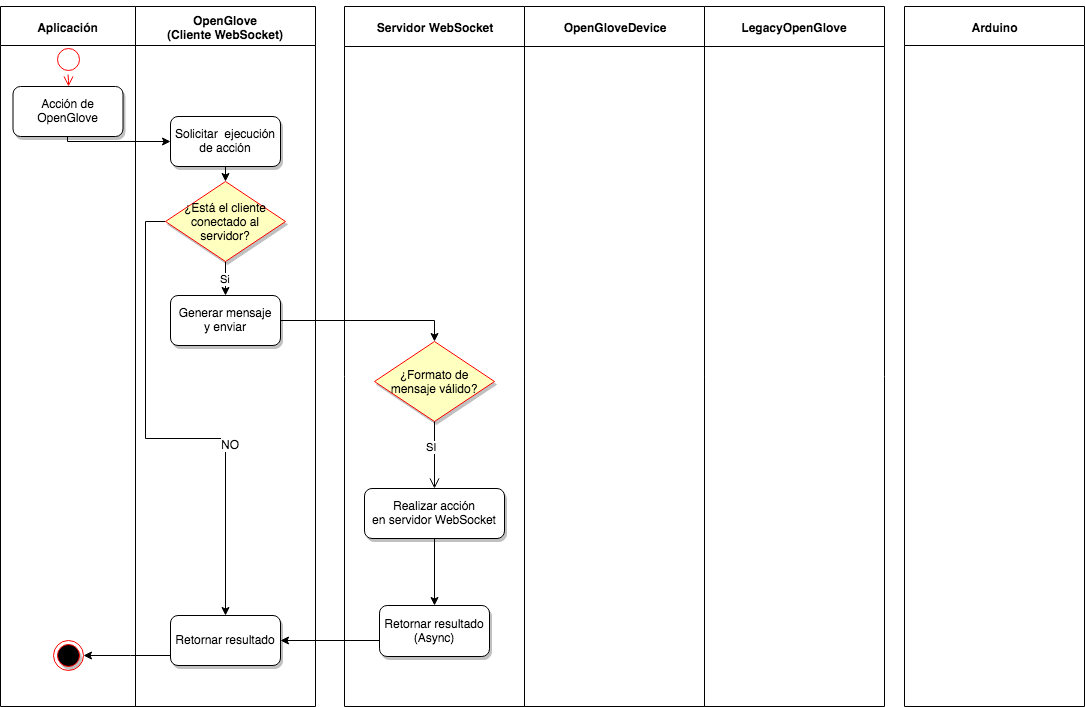
\includegraphics[width=1.0\textwidth]{images/chapter04/ActivityDiagrams-OpenGloveActions-1.png} 
   	\captionsetup{justification=centering}
    \caption[Diagrama de actividad de los métodos aplicados sobre el servidor WebSocket]{Diagrama de actividad de los métodos aplicados sobre el servidor WebSocket\\Fuente: Elaboración propia (2018)}
    \label{fig:activity-diagrams-1-websocket-server}
  \end{center}
\end{figure}





\subsection{Métodos aplicados sobre instancias de OpenGloveDevice}
\label{subsection:method-openglove-device}
Los métodos que pueden ser aplicados sobre la instancia de la clase OpenGloveDevice en el servidor WebSocket se muestran en la Figura \ref{fig:methods-2-openglove-device}. Estos métodos son ejecutados por la aplicación que utiliza una instancia de OpenGlove, realizando la acción sobre la instancia de OpenGloveDevice en el servidor WebSocket, pasando por las capas intermedias del cliente y el servidor WebSocket. El comportamiento de estos métodos se puede apreciar en el diagrama de actividades de la Figura \ref{fig:activity-diagrams-2-openglove-device}.


\begin{figure}[H]
  \begin{center} 
\begin{lstlisting}
// OpenGloveActions: OpenGlove Instances
public void ConnectToBluetoothDevice();
public void DisconnectFromBluetoothDevice();
public void AddActuator(int region, int positivePin, int negativePin);
public void AddActuators(List<int> regions, List<int> positivePins, List<int> negativePins);
public void AddFlexor(int region, int pin);
public void AddFlexors(List<int> regions, List<int> pins);
public void SetThreshold(int value);
public void SetIMUStatus(bool status);
public void SetRawData(bool status);
public void SetIMUChoosingData(int value);
public void SetLoopDelay(int value);
\end{lstlisting}
   	\captionsetup{justification=centering}
    \caption[Métodos aplicados sobre instancias de OpenGloveDevice]{Métodos aplicados sobre instancias de OpenGloveDevice\\Fuente: Elaboración propia (2018)}
    \label{fig:methods-2-openglove-device}
  \end{center}
\end{figure}

\begin{figure}[H]
  \begin{center} 
   	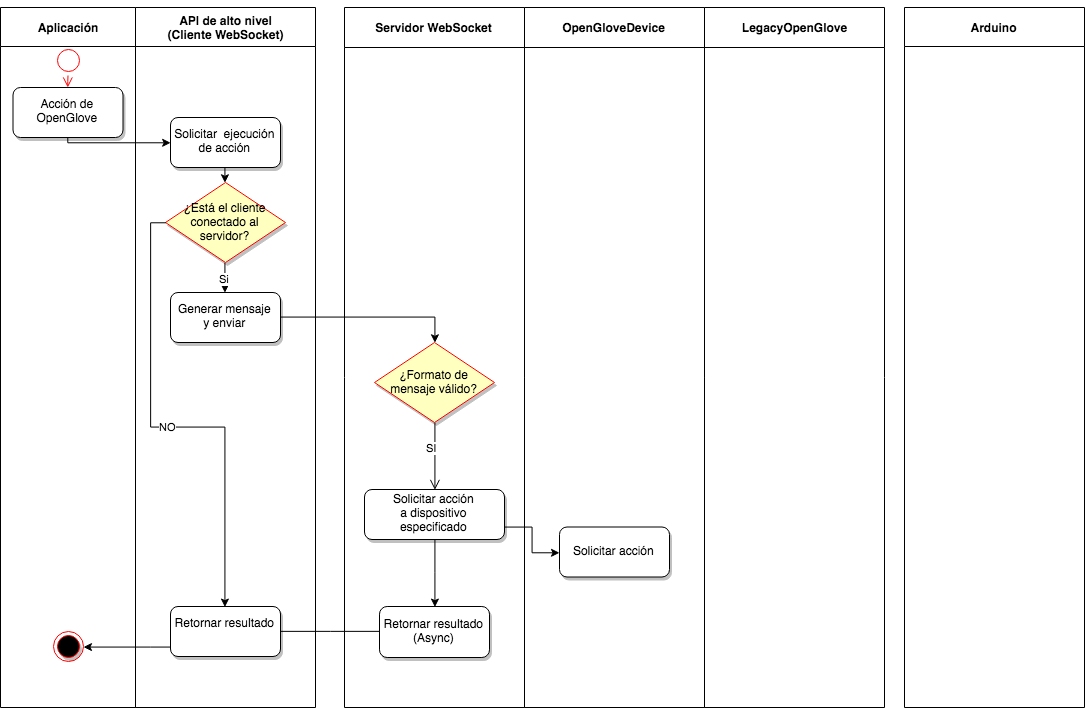
\includegraphics[width=1.0\textwidth]{images/chapter04/ActivityDiagrams-OpenGloveActions-2.png} 
   	\captionsetup{justification=centering}
    \caption[Diagrama de actividades de las acciones OpenGlove sobre instancias de OpenGloveDevice en servidor]{Diagrama de actividades de las acciones OpenGlove sobre instancias de OpenGloveDevice en servidor\\Fuente: Elaboración propia (2018)}
    \label{fig:activity-diagrams-2-openglove-device}
  \end{center}
\end{figure}



\subsection{Métodos aplicados sobre el software de control Arduino}
\label{subsection:method-openglove-arduino}
Los métodos que pueden ser aplicados sobre el software de control Arduino se muestran en la Figura \ref{fig:methods-3-openglove-arduino}. Estos métodos son ejecutados por la aplicación que utiliza una instancia de OpenGlove, realizando la acción sobre el software de control Arduino. Estos métodos generan cambios en el dispositivo Arduino. Para realizar la acción se pasa por las capas intermedias del cliente, el servidor WebSocket y la instancia de OpenGloveDevice que administra la conexión con Arduino. El comportamiento de estos métodos se puede apreciar en el diagrama de actividades de la Figura \ref{fig:activity-diagrams-3-openglove-arduino}.


\begin{figure}[H]
  \begin{center} 
\begin{lstlisting}
// OpenGloveActions: Software of Control Arduino
public void Start();
public void Stop();
public void RemoveActuator(int region);
public void RemoveActuators(List<int> regions);
public void ActivateActuators(List<int> regions, List<string> intensities);
public void ActivateActuatorsTimeTest(List<int> regions, List<string> intensities);
public void TurnOnActuators();
public void TurnOffActuators();
public void TurnOnFlexors();
public void TurnOffFlexors();
public void ResetActuators();
public void RemoveFlexor(int region);
public void RemoveFlexors(List<int> regions);
public void CalibrateFlexors();
public void ConfirmCalibration();
public void ResetFlexors();
public void StartIMU();
public void ReadOnlyAccelerometerFromIMU();
public void ReadOnlyGyroscopeFromIMU();
public void ReadOnlyMagnetometerFromIMU();
public void ReadOnlyAttitudeFromIMU();
public void ReadAllDataFromIMU();
public void TurnOnIMU();
public void TurnOffIMU();
public void GetOpenGloveArduinoVersionSoftware();
\end{lstlisting}
   	\captionsetup{justification=centering}
    \caption[Métodos aplicados sobre el software de control Arduino]{Métodos aplicados sobre el software de control Arduino\\Fuente: Elaboración propia (2018)}
    \label{fig:methods-3-openglove-arduino}
  \end{center}
\end{figure}



\begin{figure}[H]
  \begin{center} 
   	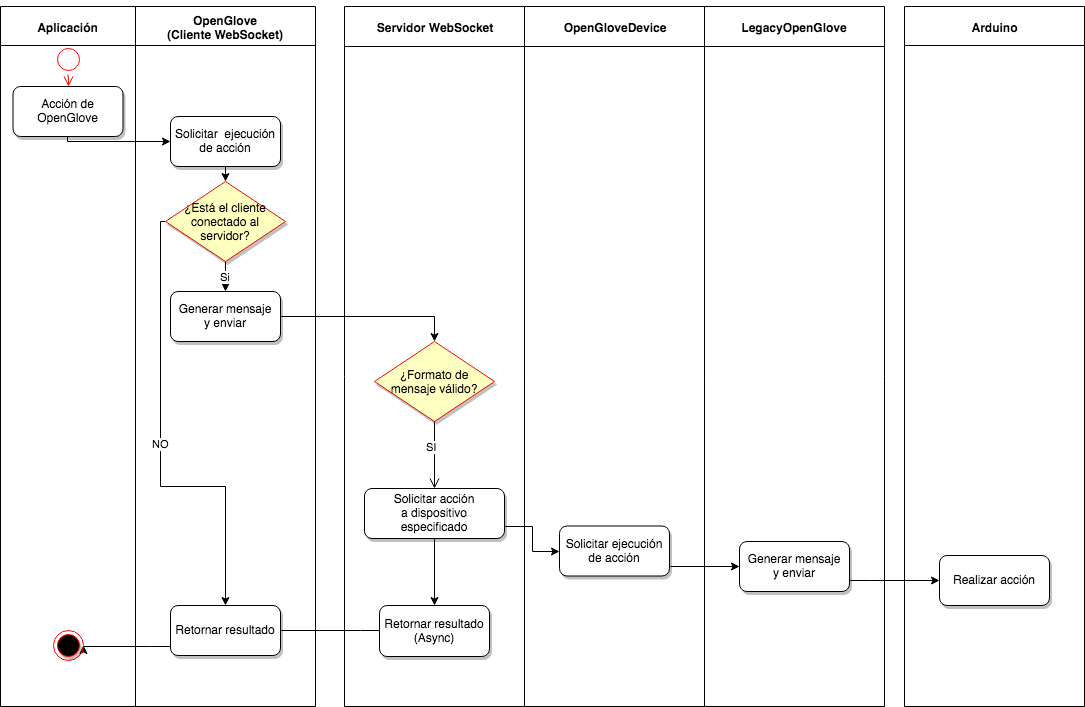
\includegraphics[width=1.0\textwidth]{images/chapter04/ActivityDiagrams-OpenGloveActions-3.png} 
   \captionsetup{justification=centering}
    \caption[Diagrama de actividades de los métodos aplicados sobre el software de control Arduino]{Diagrama de actividades de los métodos aplicados sobre el software de control Arduino\\Fuente: Elaboración propia (2018)}
    \label{fig:activity-diagrams-3-openglove-arduino}
  \end{center}
\end{figure}


\subsection{Escuchando mensajes provenientes de Arduino}
\label{subsection:reading-openglove-arduino}
Este comportamiento ocurre cuando se ha inicializado por lo menos un flexor y/o se ha inicializado e iniciado la IMU. La Figura \ref{fig:methods-4-listening-arduino}, muestra el formato de los métodos que deben ser implementados por los objetos que utilicen instancias de la clase OpenGlove. El comportamiento de estos métodos se aprecia en el Diagrama de actividades de la Figura \ref{fig:activity-diagrams-4-ListeningMessagesFromArduino}

\begin{figure}[H]
  \begin{center}
\begin{lstlisting}
// OpenGloveActions: Listening messages from Arduino Control Software
// For use in API C#: subcribe to event with your own method
// For use in API Java: implements public interface with lambdas or method references
public void OnTimeTestServerLatencyActivateActuatorsReceived(long nanoSeconds);
public void OnTimeTestArduinoLatencyActivateActuatorsReceived(long microSeconds);
public void OnFlexorValueReceived(int region, int value);
public void OnAccelerometerValuesReceived(float ax, float ay, float az);
public void OnGyroscopeValuesReceived(float gx, float gy, float gz);
public void OnMagnometerValuesReceived(float mx, float my, float mz);
public void OnAttitudeValuesReceived(float pitch, float roll, float yaw);
public void OnAllIMUValuesReceived(float ax, float ay, float az, float gx, float gy, float gz, float mx, float my, float mz);
public void OnInfoMessagesReceived(string message);
\end{lstlisting}
   	\captionsetup{justification=centering}
    \caption[Lectura de mensajes provenientes de Arduino]{Lectura de mensajes provenientes de Arduino\\Fuente: Elaboración propia (2018)}
    \label{fig:methods-4-listening-arduino}
  \end{center}
\end{figure}

\begin{figure}[H]
  \begin{center} 
   	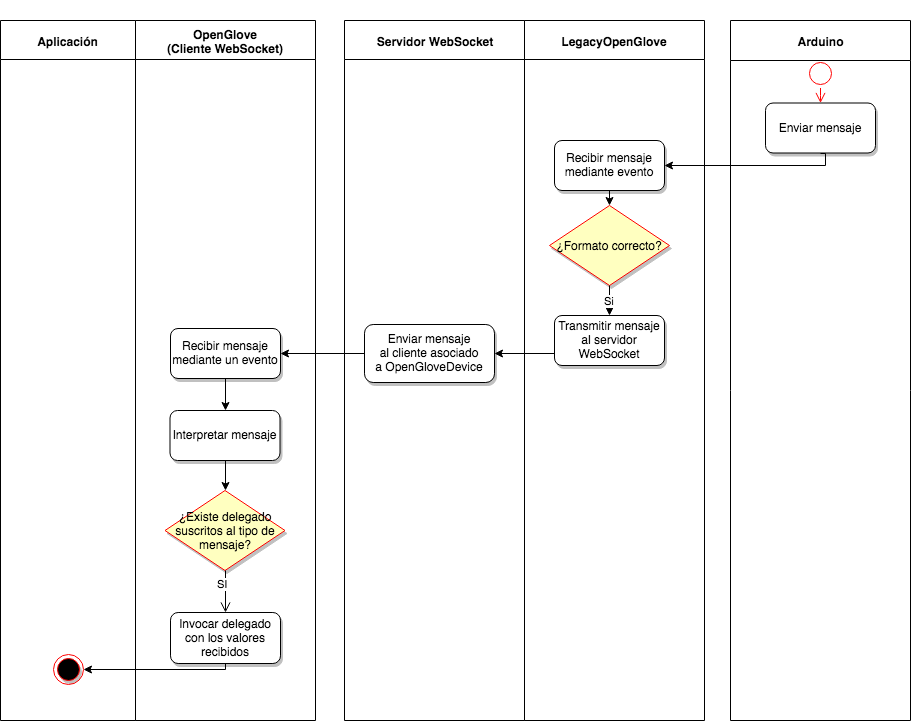
\includegraphics[width=1.0\textwidth]{images/chapter04/ActivityDiagrams-ListeningMessagesFromArduino.png} 
   	\captionsetup{justification=centering}
    \caption[Diagrama de actividades de la lectura de mensajes provenientes de Arduino]{Diagrama de actividades de la lectura de mensajes provenientes de Arduino\\Fuente: Elaboración propia (2018)}
    \label{fig:activity-diagrams-4-ListeningMessagesFromArduino}
  \end{center}
\end{figure}

\subsection{Escuchando el estado de conexión del dispositivo Bluetooth}
\label{subsection:reading-bluetooth-device-state}

Para actualizar el estado de la conexión Bluetooth en las APIs de alto nivel, el hilo que administra dicha conexión, debe enviar  actualizaciones del estado de conexión o desconexión con los dispositivos. Cuando el estado del socket está conectado se envía un mensaje  \textit{``b,True"}  y cuando no, se envía \textit{``b,False"}. La Figura \ref{fig:methods-5-listening-bluetoothdevice-state}, muestra el método que se debe implementar para obtener los cambios de estado de la conexión Bluetooth.  El comportamiento de activación de estos métodos se puede apreciar en el diagrama de actividades de la Figura \ref{fig:activity-diagrams-5-listening-bluetoothdevice-state}.

\begin{figure}[H]
  \begin{center}
\begin{lstlisting}
// OpenGloveActions: Listening Bluetooth device connection state messages
// For use in API C#: subcribe to event with your own method
// For use in API Java: implements public interface with lambdas or method references
public void OnBluetoothDeviceConnectionStateChanged(bool isConnected);
\end{lstlisting}
   	\captionsetup{justification=centering}
    \caption[Lectura del estado de conexión del dispositivo Bluetooth]{Lectura del estado de conexión del dispositivo Bluetooth\\Fuente: Elaboración propia (2018)}
    \label{fig:methods-5-listening-bluetoothdevice-state}
  \end{center}
\end{figure}

\begin{figure}[H]
  \begin{center} 
   	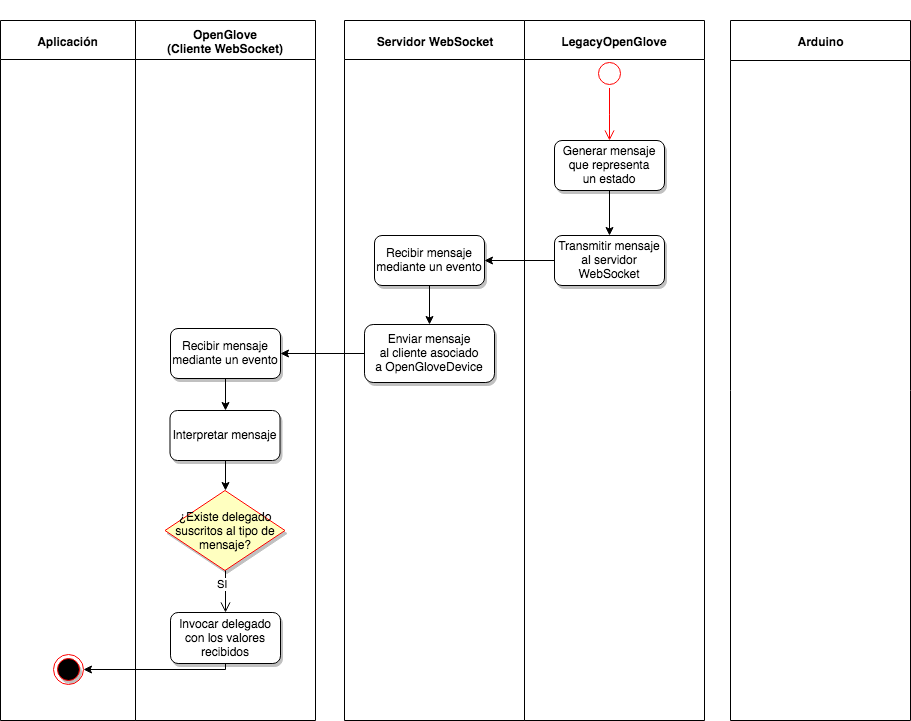
\includegraphics[width=1.0\textwidth]{images/chapter04/ActivityDiagrams-ListeningMessagesFromOpenGloveDevice.png} 
   	\captionsetup{justification=centering}
    \caption[Diagrama de actividades del método que escucha la conexión del dispositivo Bluetooth]{Diagrama de actividades del método que escucha la conexión del dispositivo Bluetooth\\Fuente: Elaboración propia (2018)}
    \label{fig:activity-diagrams-5-listening-bluetoothdevice-state}
  \end{center}
\end{figure}


\subsection{Escuchando el estado de conexión del cliente WebSocket}
\label{subsection:listening-openglove-arduino}
Para notificar el estado de la conexión del cliente WebSocket en las APIs de alto nivel, se invoca el método OnWebSocketConnectionStateChanged, cada vez que ocurre un cambio utilizando OnOpen y OnClose de la API WebSocket. La Figura \ref{fig:methods-6-listening-websocket-state}, muestra el método que debe ser implementado para escuchar el estado de conexión del cliente WebSocket. El comportamiento de este método se puede apreciar en el diagrama de actividades de la Figura \ref{fig:activity-diagrams-6-listening-websocket-state}.


\begin{figure}[H]
  \begin{center}
\begin{lstlisting}
// OpenGloveActions: Listening WebSocket client connection state messages
// For use in API C#: subcribe to event with your own method
// For use in API Java: implements public interface with lambdas or method references
public void OnWebSocketConnectionStateChanged(bool isConnected);
\end{lstlisting}
   	\captionsetup{justification=centering}
    \caption[Lectura del estado de conexión del cliente WebSocket]{Lectura del estado de conexión del cliente WebSocket\\Fuente: Elaboración propia (2018)}
    \label{fig:methods-6-listening-websocket-state}
  \end{center}
\end{figure}


\begin{figure}[H]
  \begin{center} 
   	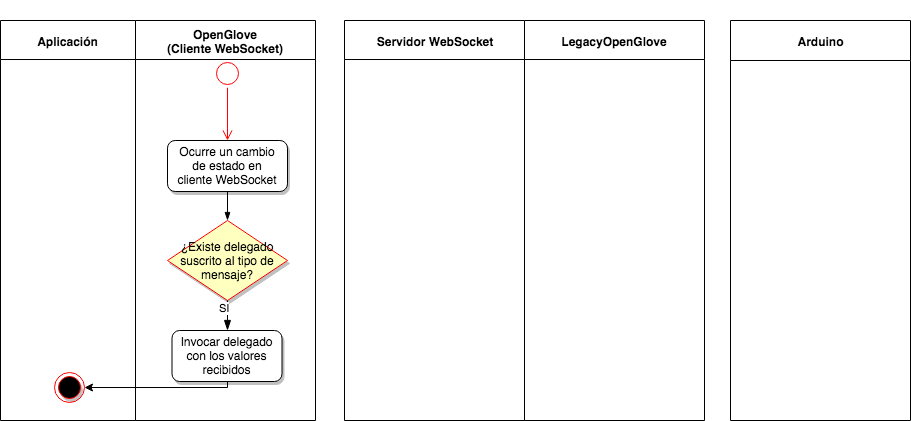
\includegraphics[width=1.0\textwidth]{images/chapter04/ActivityDiagrams-ListeningFromWebSocketClient.png} 
   	\captionsetup{justification=centering}
    \caption[Diagrama de actividades del método que escucha la conexión del dispositivo Bluetooth]{Diagrama de actividades del método que escucha la conexión del dispositivo Bluetooth\\Fuente: Elaboración propia (2018)}
    \label{fig:activity-diagrams-6-listening-websocket-state}
  \end{center}
\end{figure}
	\section{Aspectos de implementación}


\subsection{Desarrollo multiplataforma en Xamarin.Forms}
De los resultados de la comparación en la Sección \ref{section:native-vs-crossplartform} entre desarrollo nativo en Android con Android Studio y  Android con Xamarin.Forms, se obtuvo que los rendimientos no eran muy diferentes entre si, por tanto, se optó por el uso de Xamarin.Forms, ya que provee soporte multiplataforma y permite que el proyecto pueda ser utilizado en otras plataformas en un futuro, utilizando las APIs y bibliotecas nativas que permitan comunicación tanto Bluetooth como WebSocket.




\subsection{API C\# bajo nivel}
En la Sección \ref{subseccion-estructura-api-ll}, se detalla sobre la estructura de OpenGloveDevice que corresponde a la API de bajo nivel C\#. Respecto a la implementación, se debe mencionar el uso de \textit{DependencyService}\footnote{DependencyService: \url{https://docs.microsoft.com/en-us/xamarin/xamarin-forms/app-fundamentals/dependency-service/introduction}} de Xamarin.Forms, el cual permite realizar diferentes implementaciones de una interfaz referenciada en el proyecto principal, a los demás proyectos asociados (iOS, Android, UWP, etc.). Para ello se requiere la declaración de una interfaz en el código compartido (proyecto principal), segundo, realizar una implementación de la interfaz en cada proyecto por plataforma, cada implementación debe ser registrada en \textit{DependencyService} para que esta sea cargada en tiempo de ejecución. Finalmente en el código compartido, se debe llamar explícitamente a \textit{DependencyService} para hacer uso de ella.


\subsection{Servidor WebSocket}




\subsection{Software de configuración}



\subsection{APIs}
	%\subsubsection{Kotlin}
	%\subsubsection{Objetive C}
	%\subsubsection{Swift}
	%\subsubsection{C++}
	
	\subsubsection{Java}

	\subsubsection{C\#}
    
	\section{Resumen}
Este capítulo abordó el diseño e implementación de la solución propuesta, detallando la arquitectura adoptada, su comportamiento y aspectos importantes de la implementación del diseño. Con ello se logró definir y utilizar una arquitectura con diferentes capas de abstracción, utilizando clientes WebSocket como representación de dispositivos OpenGlove, para poder enviar y recibir información desde el servidor que brinda la mayoría de las funcionalidades. Gracias a esto se logró minimizar la complejidad de las APIs de alto nivel, permitiendo a la comunidad de desarrolladores crear sus propias APIs de alto nivel para otros lenguajes, teniendo como base las hechas con C\# y Java.
		
\newpage
\chapter{Evaluación técnica}
En este capítulo se detallan las evaluaciones técnicas realizadas en el proyecto. Primero se muestran los resultados de las evaluaciones de motores y flexores de la aplicación nativa (tercer prototipo) y multiplataforma (cuarto prototipo), con los cuales se decide el uso de Xamarin.Forms. En segundo lugar se muestran y analizan los resultados de los tiempos de activación de los motores para las APIs desarrolladas en C\# y Java. En tercer lugar se muestran y analizan los resultados obtenidos de los tiempo de lectura de datos desde los flexores e IMU juntos para las APIs antes mencionadas. Finalmente se realiza un resumen sobre los resultados obtenidos en las evaluaciones técnicas del proyecto.
	\section{Evaluación aplicaciones nativa y multiplataforma}

A continuación se detalla la evaluación de los prototipos 3 y 4 ya expuestos en la Sección 3.2, los cuales poseen las mismas funcionalidades pero desarrollados con distintas herramientas, el primero utilizando el IDE Android Studio para desarrollar con el SDK nativo de android (desde ahora Droid) y el segundo prototipo utilizando el IDE VisualStudio Community en un proyecto Xamarin.Forms (desde ahora Xamarin). Ambos prototipos fueron modificados para realizar la siguiente evaluación que consta de 1,000 muestras y su almacenamiento en la memoria interna para la cantidad de motores y flexores del hardware disponible. Las pruebas fueron realizadas en el dispositivo Samsung Galaxy S5 mini y Nexus 5 ya señalados en el Capítulo 1. Para el análisis de latencia de los motores, se considerando su tiempo de activación y desactivación con una precisión de nanosegundos ($ns$), transformando los resultados a microsegundos ($\mu s$).  Por tanto el umbral límite de 60 milisegundos ($ms$) es equivalente a 60,000 $\mu s$ ó 60,000,000 $ns$ .

\subsection{Prototipo 3 : Droid - Galaxy}

\subsubsection{Motores}

Se realizaron pruebas desde uno a cinco motores , el resumen de los resultados para las pruebas de activación de los motores se encuentra en la Tabla \ref{table:motor-droid-galaxy}. La Figura \ref{fig:droid-galaxy-hist-motors}, muestra los histogramas de las latencias obtenidas al mandar los mensajes de activación y desactivación, siendo la gráfica para dos motores el único con una asimetría (Skewness) negativa, lo que indica que la cola de la distribución de los datos está orientada a la izquierda, por tanto la media de la distribución se encuentra desplazada a la derecha. Para las demás pruebas realizadas se obtuvieron asimetrías positivas, lo que indica que la cola de la distribución se encuentra a la derecha, por tanto su media se encuentra desplazada a la izquierda. Esto se ve reflejado en los gráficos de cajas de la Figura \ref{fig:droid-galaxy-boxplot-motors}. Las gráficas de Q-Q (quantile-quantile) mostradas en la Figura \ref{fig:droid-galaxy-QQ-motors}, demuestran que la curva no sigue estrictamente una distribución normal, pero los gráfico Q-Q de la misma figura, para para dos, cuatro y cinco motores muestra resultados cercanos a la normal exceptuando los valores atípicos, los cuales pueden ser apreciados también en sus respectivas gráficas de cajas. Finalmente la Curtosis (Kurtosis) de todas las pruebas fue positiva, lo que indica que las colas de estas distribuciones son más pesadas que la de una distribución normal, es decir, en comparación a ella concentran mayor cantidad de datos en las colas.

% {START} RESUME TABLE ---------------------------------
%\caption[Resumen resultado pruebas motor Droid-Galaxy]{Resumen resultado pruebas motor Droid-Galaxy \\ Fuente: Elaboración propia (2018)}
%\label{table:motor-droid-galaxy} 

% Table created by stargazer v.5.2.2 by Marek Hlavac, Harvard University. E-mail: hlavac at fas.harvard.edu
% Date and time: Tue, Jul 03, 2018 - 19:28:30
% Requires LaTeX packages: dcolumn 
\begin{table}[!htbp] \centering 
\caption[Resumen resultado pruebas motor Droid-Galaxy]{Resumen resultado pruebas motor Droid-Galaxy  en $\mu s$\\ Fuente: Elaboración propia (2018)}
\label{table:motor-droid-galaxy}
\begin{tabular}{@{\extracolsep{5pt}} D{.}{.}{-3} D{.}{.}{-3} D{.}{.}{-3} D{.}{.}{-3} D{.}{.}{-3} D{.}{.}{-3} D{.}{.}{-3} D{.}{.}{-3} } 
\\[-1.8ex]\hline 
\hline \\[-1.8ex] 
\multicolumn{1}{c}{Motors} & \multicolumn{1}{c}{Mean} & \multicolumn{1}{c}{Median} & \multicolumn{1}{c}{Min} & \multicolumn{1}{c}{Max} & \multicolumn{1}{c}{Std. Dev.} & \multicolumn{1}{c}{Skewness} & \multicolumn{1}{c}{Kurtosis} \\ 
\hline \\[-1.8ex] 
1 & 245.345 & 170.156 & 135.469 & 681.354 & 141.369 & 1.336 & 3.376 \\ 
2 & 263.026 & 272.031 & 192.084 & 357.083 & 36.334 & -0.114 & 2.965 \\ 
3 & 570.168 & 375.026 & 313.802 & 1,576.875 & 337.726 & 1.257 & 2.911 \\ 
4 & 418.957 & 424.843 & 304.688 & 668.750 & 61.357 & 0.417 & 4.613 \\ 
5 & 484.390 & 497.240 & 353.073 & 724.479 & 78.401 & 0.221 & 3.303 \\ 
\hline \\[-1.8ex] 
\end{tabular} 
\end{table} 
% {END} RESUME TABLE ---------------------------------


\begin{figure}
 \begin{center} 
   	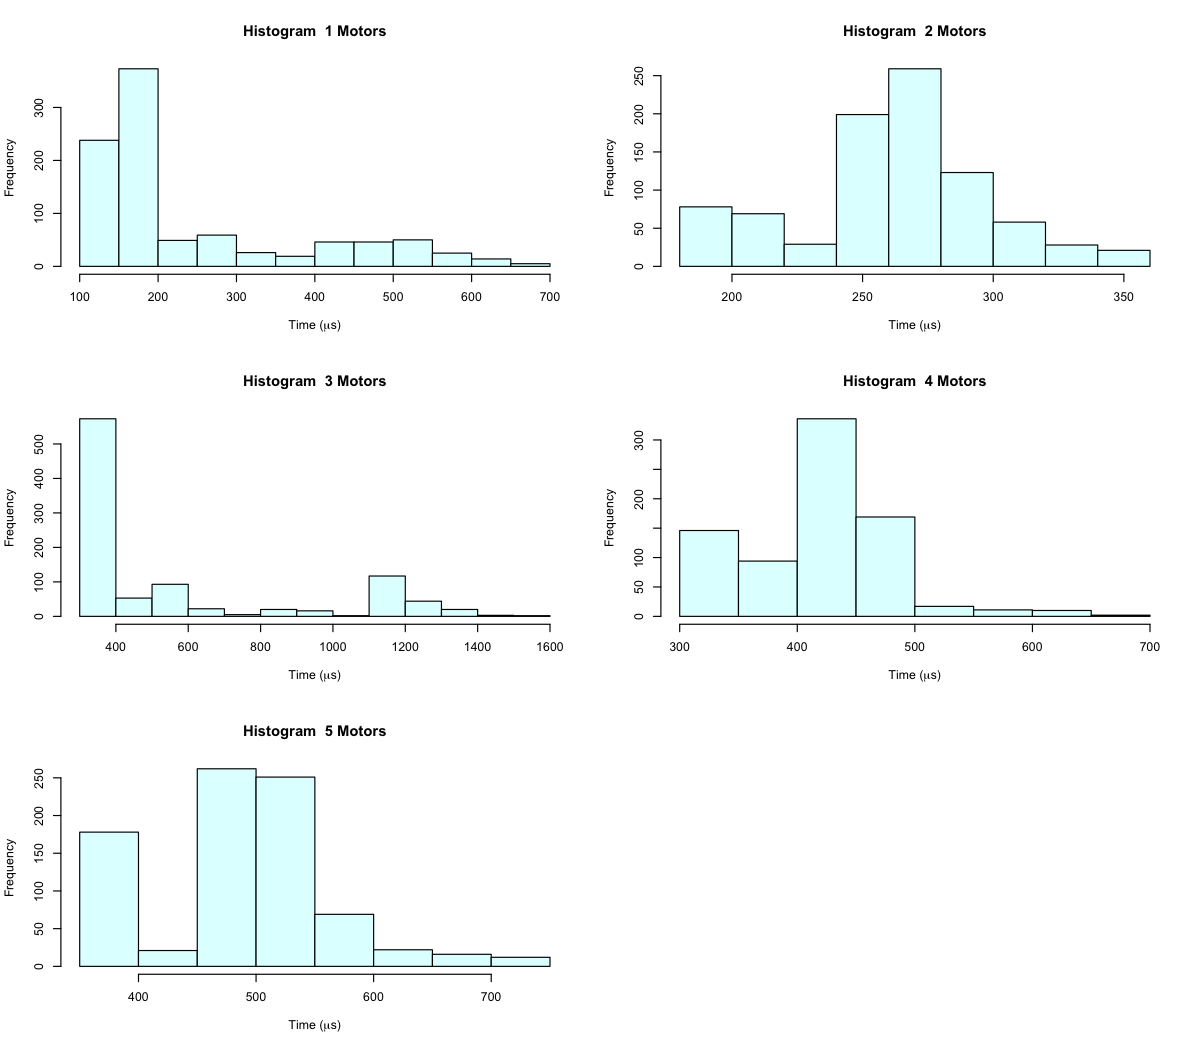
\includegraphics[width=1.0\textwidth]{evaluation/graphics/Droid/Galaxy/HistMotorsDroidGalaxy.png} 
    \caption[Histogramas de motores Droid-Galaxy]{Histogramas de motores  Droid-Galaxy\\Fuente: elaboración propia (2018)} 
    \label{fig:droid-galaxy-hist-motors}
  \end{center}
\end{figure}

\begin{figure}[H]
  \begin{center} 
   	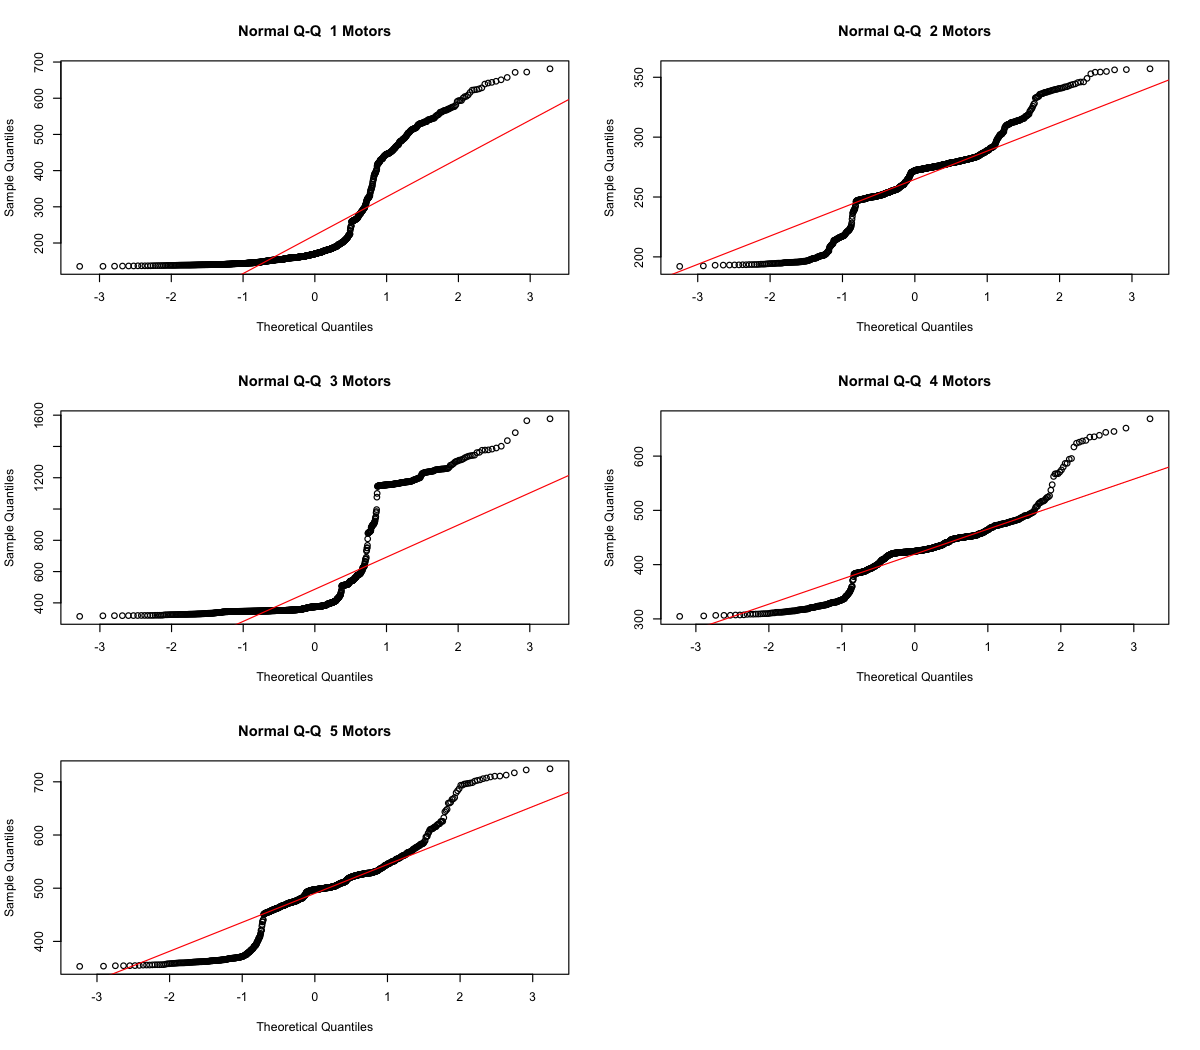
\includegraphics[width=1.0\textwidth]{evaluation/graphics/Droid/Galaxy/NormalQQMotorsDroidGalaxy.png} 
    \caption[Gráfico QQ de motores Droid-Galaxy]{Gráficos QQ de motores Droid-Galaxy\\Fuente: elaboración propia (2018)} 
    \label{fig:droid-galaxy-QQ-motors}
  \end{center}
\end{figure}

\begin{figure}[H]
  \begin{center} 
   	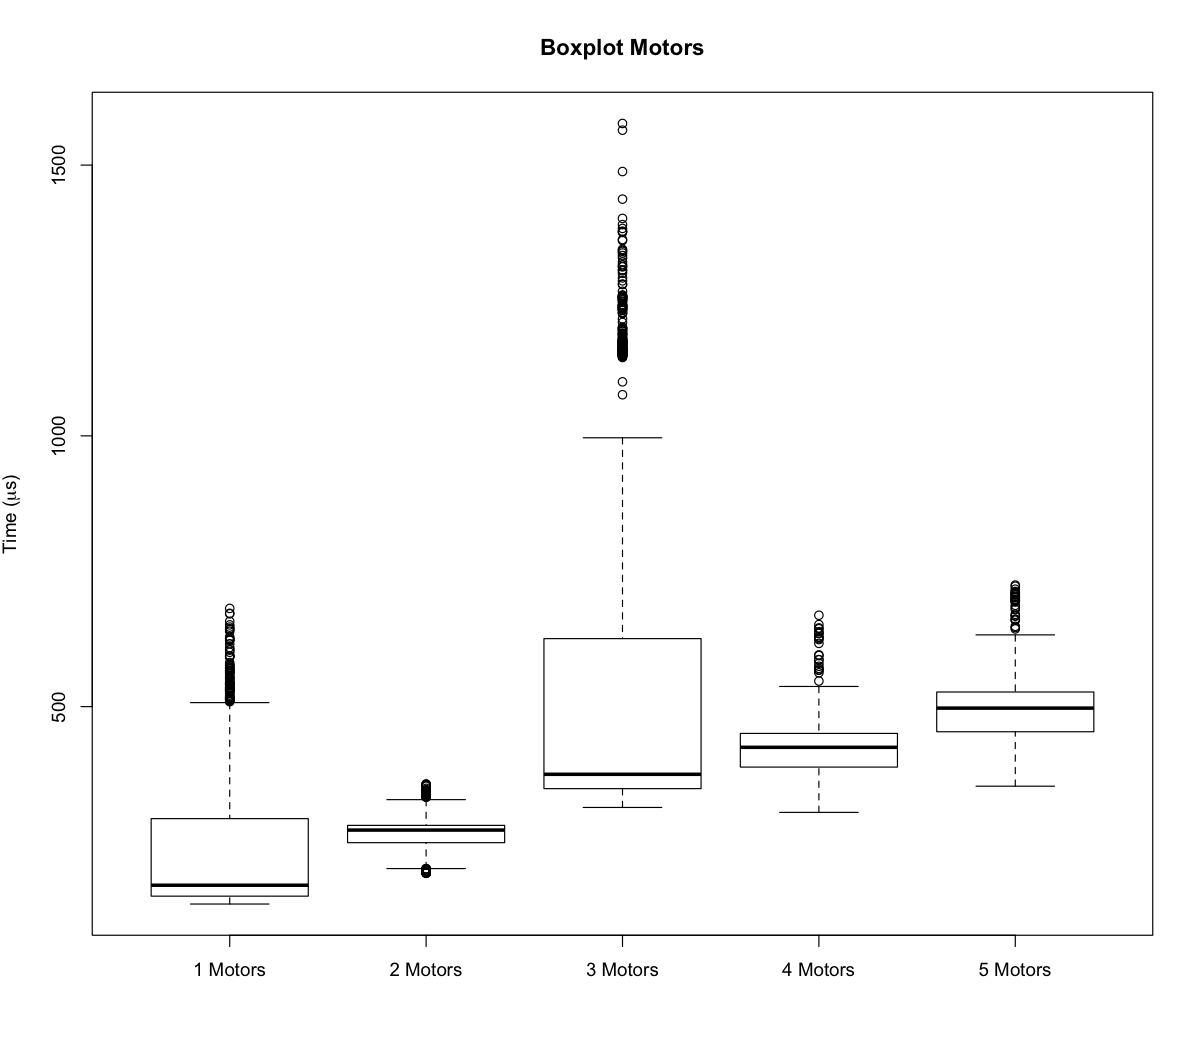
\includegraphics[width=0.8\textwidth]{evaluation/graphics/Droid/Galaxy/BoxplotMotorsDroidGalaxy.png} 
    \caption[Gráficos de cajas de motores Droid-Galaxy]{Gráficos de cajas de motores Droid-Galaxy\\Fuente: elaboración propia (2018)} 
    \label{fig:droid-galaxy-boxplot-motors}
  \end{center}
\end{figure}



\subsubsection{Flexores}
En el caso de los flexores, se realizó solamente una prueba para la obtención de datos desde la placa Arduino, con el único flexor físico disponible. Se utilizó una API de bajo nivel en Java desarrollada, en base a la C\# de bajo nivel. El resumen de los resultados de la prueba se muestra en la Tabla \ref{table:flexor-droid-galaxy}. De la tabla se puede observar que la muestra presenta una asimetría positiva, lo que implica que la cola de la distribución se encuentra a la derecha, por tanto, la media se encuentra desplazada hacia la izquierda, su Curtosis al ser positiva indica que posee mayor concentración de datos en las colas que una distribución normal. Esto puede apreciarse en el histograma de la Figura \ref{fig:droid-galaxy-hist-flexors} en conjunto con el diagrama de cajas de la Figura \ref{fig:droid-galaxy-boxplot-flexors}. En el gráfico Q-Q de la Figura \ref{fig:droid-galaxy-QQ-flexors}, se puede apreciar que la curva no sigue una distribución normal de manera estricta, sino que presenta acercamientos a ella, en forma sinusoidal.

% {START} RESUME TABLE ---------------------------------
%\extracolsep{-11pt}
%\caption[Resumen resultado pruebas flexor Droid-Galaxy]{Resumen resultado pruebas flexor Droid-Galaxy \\ Fuente: Elaboración propia (2018)}
%\label{table:flexor-droid-galaxy}

% Table created by stargazer v.5.2.2 by Marek Hlavac, Harvard University. E-mail: hlavac at fas.harvard.edu
% Date and time: Tue, Jul 03, 2018 - 19:48:03
% Requires LaTeX packages: dcolumn 
\begin{table}[!htbp] \centering 
\caption[Resumen resultado pruebas flexor Droid-Galaxy]{Resumen resultado pruebas flexor Droid-Galaxy en $\mu s$\\ Fuente: Elaboración propia (2018)}
\label{table:flexor-droid-galaxy}
\begin{tabular}{@{\extracolsep{-11pt}} D{.}{.}{-3} D{.}{.}{-3} D{.}{.}{-3} D{.}{.}{-3} D{.}{.}{-3} D{.}{.}{-3} D{.}{.}{-3} D{.}{.}{-3} } 
\\[-1.8ex]\hline 
\hline \\[-1.8ex] 
\multicolumn{1}{c}{Motors} & \multicolumn{1}{c}{Mean} & \multicolumn{1}{c}{Median} & \multicolumn{1}{c}{Min} & \multicolumn{1}{c}{Max} & \multicolumn{1}{c}{Std. Dev.} & \multicolumn{1}{c}{Skewness} & \multicolumn{1}{c}{Kurtosis} \\ 
\hline \\[-1.8ex] 
1 & 121,879.900 & 108,551.400 & 34,473.860 & 252,435.200 & 38,318.940 & 0.658 & 2.637 \\ 
\hline \\[-1.8ex] 
\end{tabular} 
\end{table} 
% {END} RESUME TABLE ---------------------------------

\begin{figure}
 \begin{center} 
   	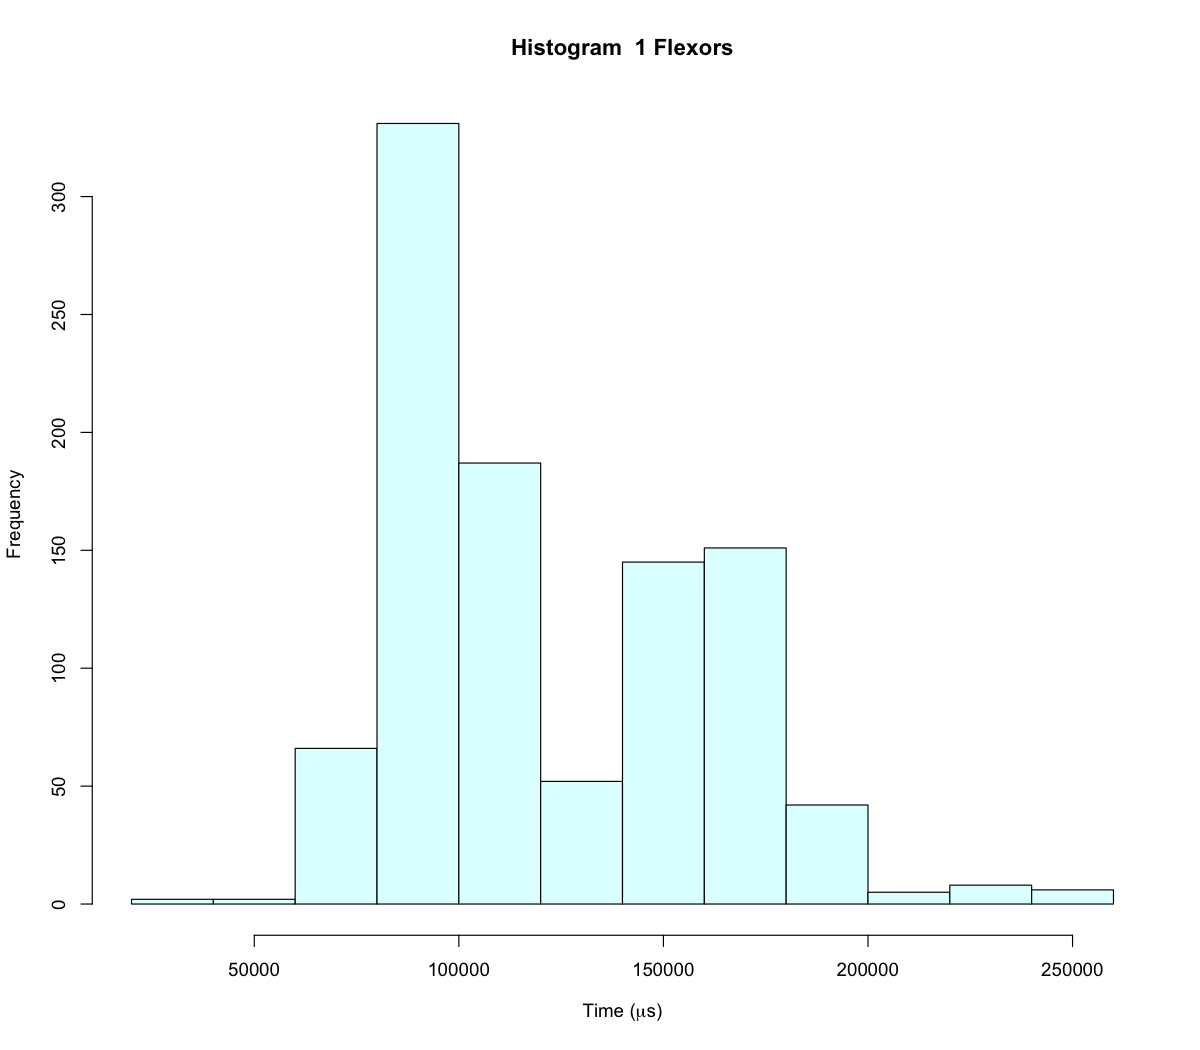
\includegraphics[width=0.5\textwidth]{evaluation/graphics/Droid/Galaxy/HistFlexorsDroidGalaxy.png} 
    \caption[Histogramas de flexores Droid-Galaxy]{Histogramas de flexores  Droid-Galaxy\\Fuente: elaboración propia (2018)} 
    \label{fig:droid-galaxy-hist-flexors}
  \end{center}
\end{figure}

\begin{figure}[H]
  \begin{center} 
   	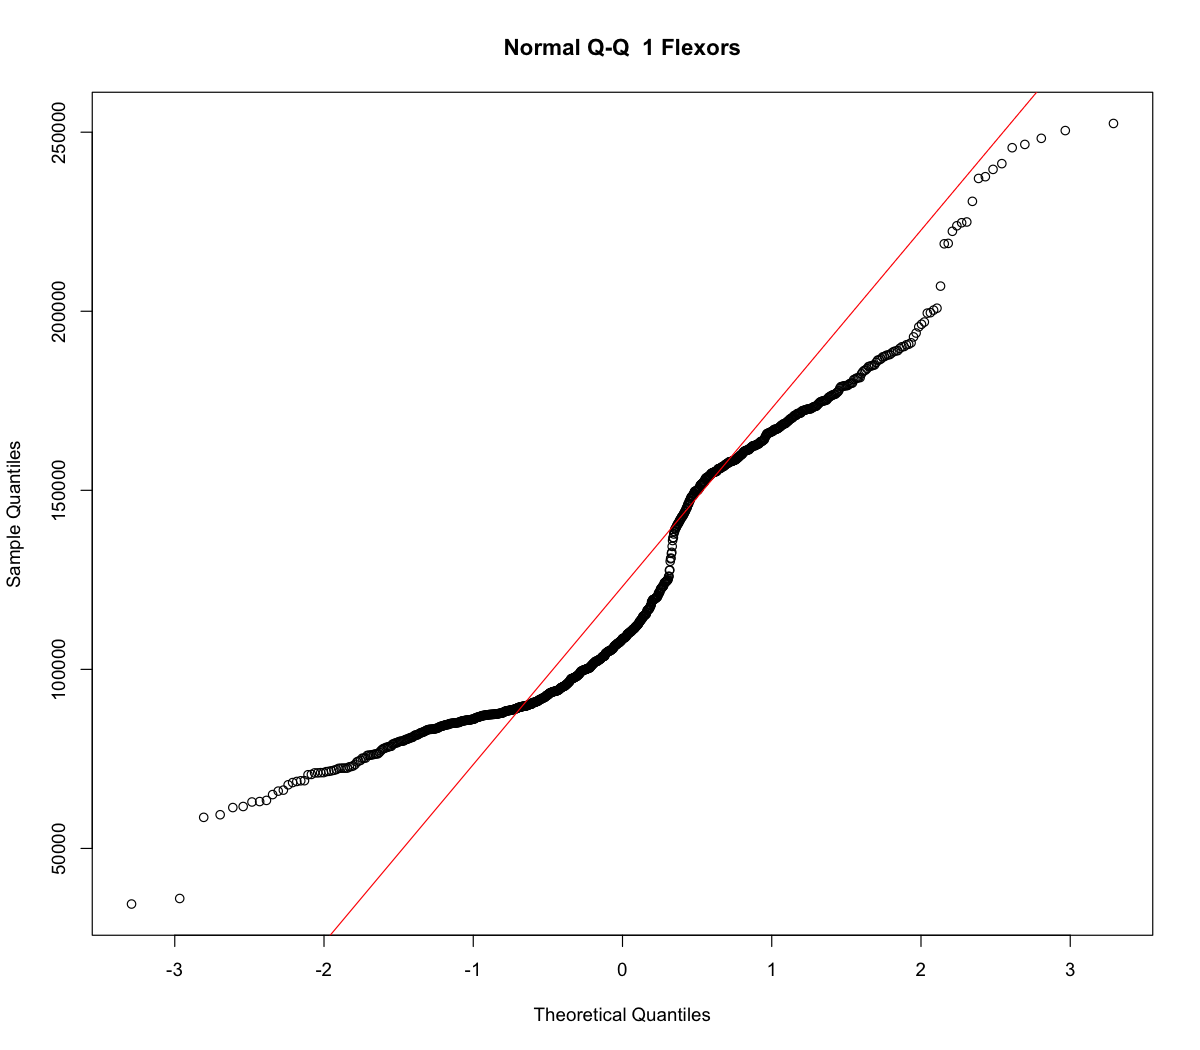
\includegraphics[width=0.5\textwidth]{evaluation/graphics/Droid/Galaxy/NormalQQFlexorsDroidGalaxy.png} 
    \caption[Gráfico QQ de flexores Droid-Galaxy]{Gráficos QQ de flexores Droid-Galaxy\\Fuente: elaboración propia (2018)} 
    \label{fig:droid-galaxy-QQ-flexors}
  \end{center}
\end{figure}

\begin{figure}[H]
  \begin{center} 
   	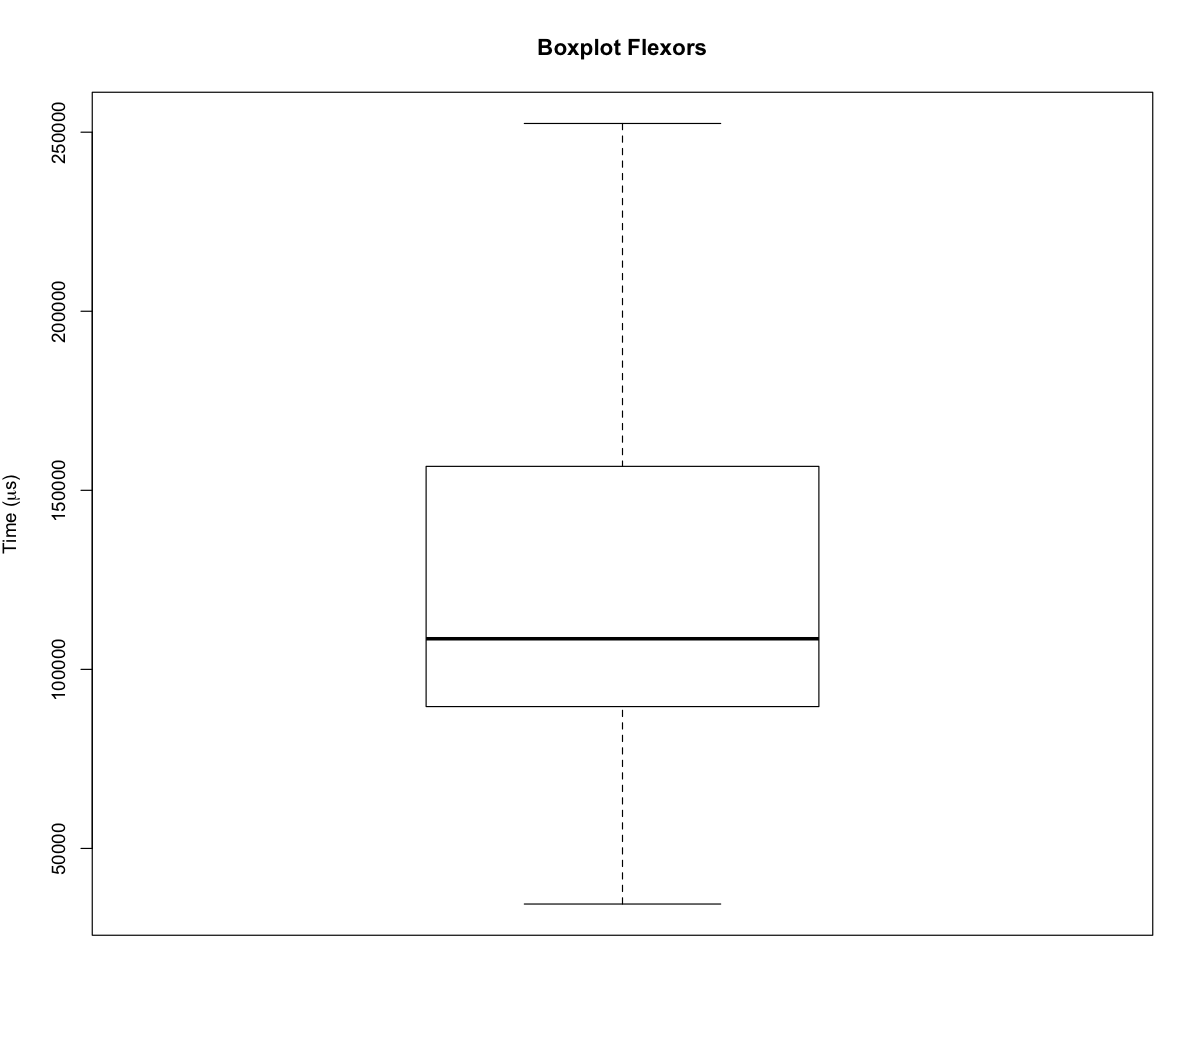
\includegraphics[width=0.5\textwidth]{evaluation/graphics/Droid/Galaxy/BoxplotFlexorsDroidGalaxy.png} 
    \caption[Gráficos de cajas de flexores Droid-Galaxy]{Gráficos de cajas de flexores Droid-Galaxy\\Fuente: elaboración propia (2018)} 
    \label{fig:droid-galaxy-boxplot-flexors}
  \end{center}
\end{figure}





\subsection{Prototipo 4: Xamarin - Galaxy}

\subsubsection{Motores}
% {START} RESUME TABLE ---------------------------------
%\caption[Resumen resultado pruebas motor Xamarin-Galaxy]{Resumen resultado pruebas motor Xamarin-Galaxy \\ Fuente: Elaboración propia (2018)}
%\label{table:motor-xamarin-galaxy}

% Table created by stargazer v.5.2.2 by Marek Hlavac, Harvard University. E-mail: hlavac at fas.harvard.edu
% Date and time: Tue, Jul 03, 2018 - 19:43:49
% Requires LaTeX packages: dcolumn 
\begin{table}[!htbp] \centering 
\caption[Resumen resultado pruebas motor Xamarin-Galaxy]{Resumen resultado pruebas motor Xamarin-Galaxy en $\mu s$ \\ Fuente: Elaboración propia (2018)}
\label{table:motor-xamarin-galaxy}
\begin{tabular}{@{\extracolsep{5pt}} D{.}{.}{-3} D{.}{.}{-3} D{.}{.}{-3} D{.}{.}{-3} D{.}{.}{-3} D{.}{.}{-3} D{.}{.}{-3} D{.}{.}{-3} } 
\\[-1.8ex]\hline 
\hline \\[-1.8ex] 
\multicolumn{1}{c}{Motors} & \multicolumn{1}{c}{Mean} & \multicolumn{1}{c}{Median} & \multicolumn{1}{c}{Min} & \multicolumn{1}{c}{Max} & \multicolumn{1}{c}{Std. Dev.} & \multicolumn{1}{c}{Skewness} & \multicolumn{1}{c}{Kurtosis} \\ 
\hline \\[-1.8ex] 
1 & 299.835 & 268.800 & 231.500 & 512 & 77.214 & 1.376 & 4.065 \\ 
2 & 367.823 & 387.100 & 282 & 600.800 & 59.888 & 0.290 & 2.832 \\ 
3 & 363.318 & 358.200 & 333 & 472.100 & 26.389 & 1.707 & 6.343 \\ 
4 & 491.245 & 506.050 & 380.800 & 785.600 & 78.420 & 0.503 & 3.042 \\ 
5 & 574.120 & 600 & 429.200 & 832.200 & 84.596 & 0.045 & 2.703 \\ 
\hline \\[-1.8ex] 
\end{tabular} 
\end{table} 
% {END} RESUME TABLE ---------------------------------

\begin{figure}
 \begin{center} 
   	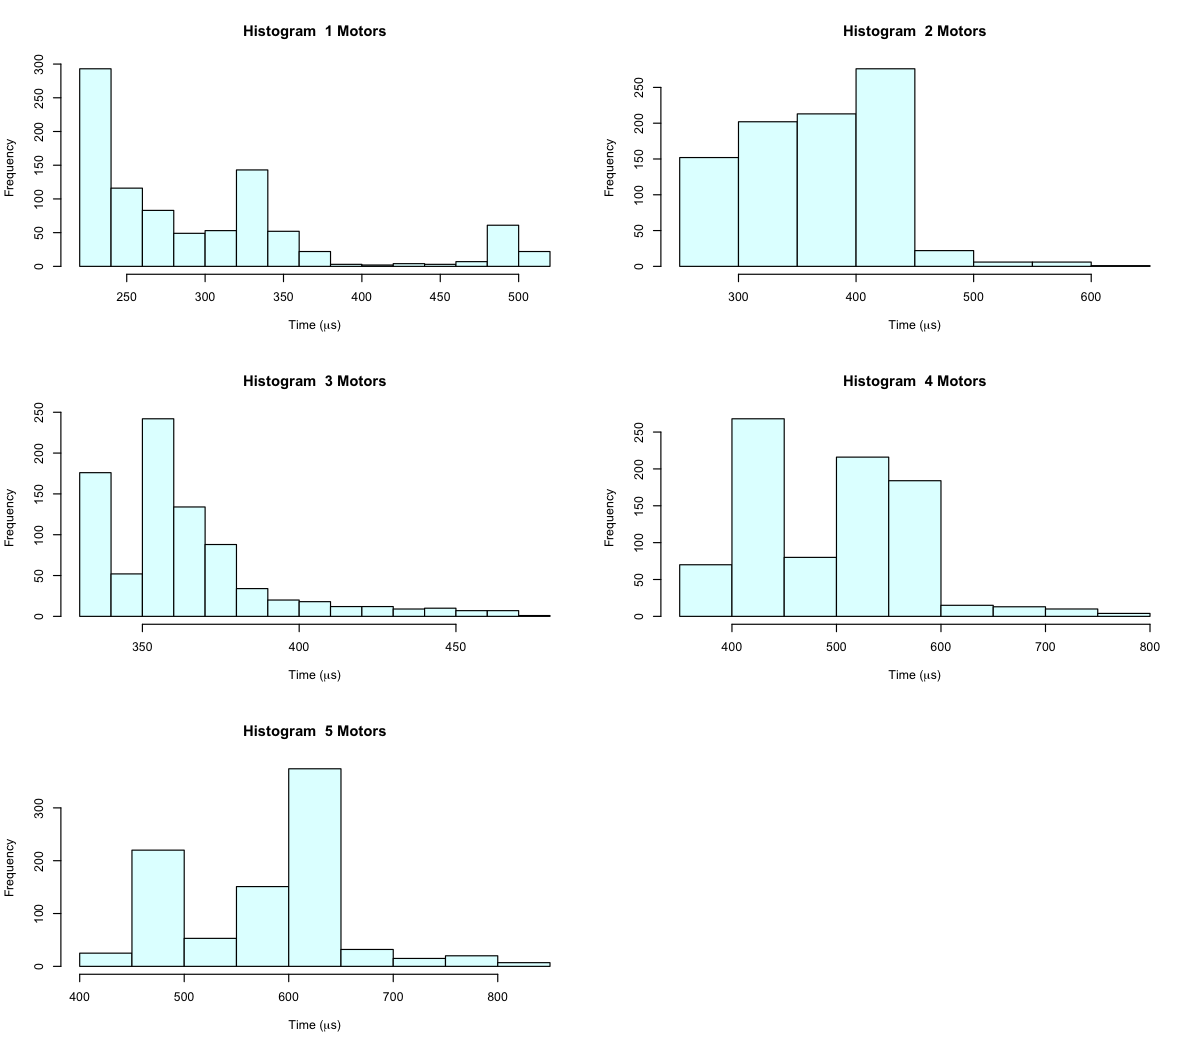
\includegraphics[width=1.0\textwidth]{evaluation/graphics/Xamarin/Galaxy/HistMotorsXamarinGalaxy.png} 
    \caption[Histogramas de motores Xamarin-Galaxy]{Histogramas de motores  Xamarin-Galaxy\\Fuente: elaboración propia (2018)} 
    \label{fig:xamarin-galaxy-hist-motors}
  \end{center}
\end{figure}

\begin{figure}[H]
  \begin{center} 
   	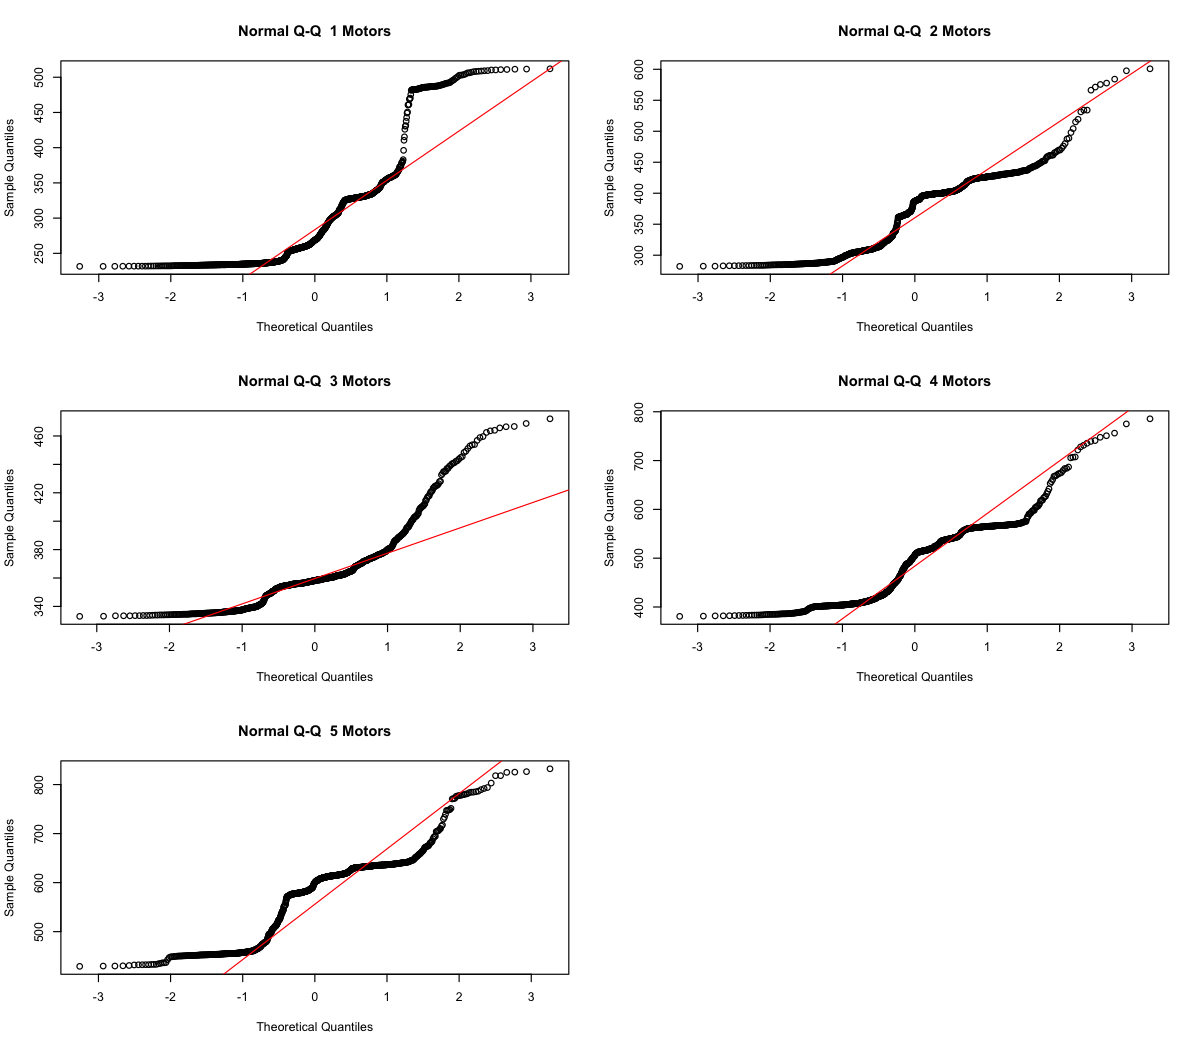
\includegraphics[width=1.0\textwidth]{evaluation/graphics/Xamarin/Galaxy/NormalQQMotorsXamarinGalaxy.png} 
    \caption[Gráfico QQ de motores Xamarin-Galaxy]{Gráficos QQ de motores Xamarin-Galaxy\\Fuente: elaboración propia (2018)} 
    \label{fig:xamarin-galaxy-QQ-motors}
  \end{center}
\end{figure}

\begin{figure}[H]
  \begin{center} 
   	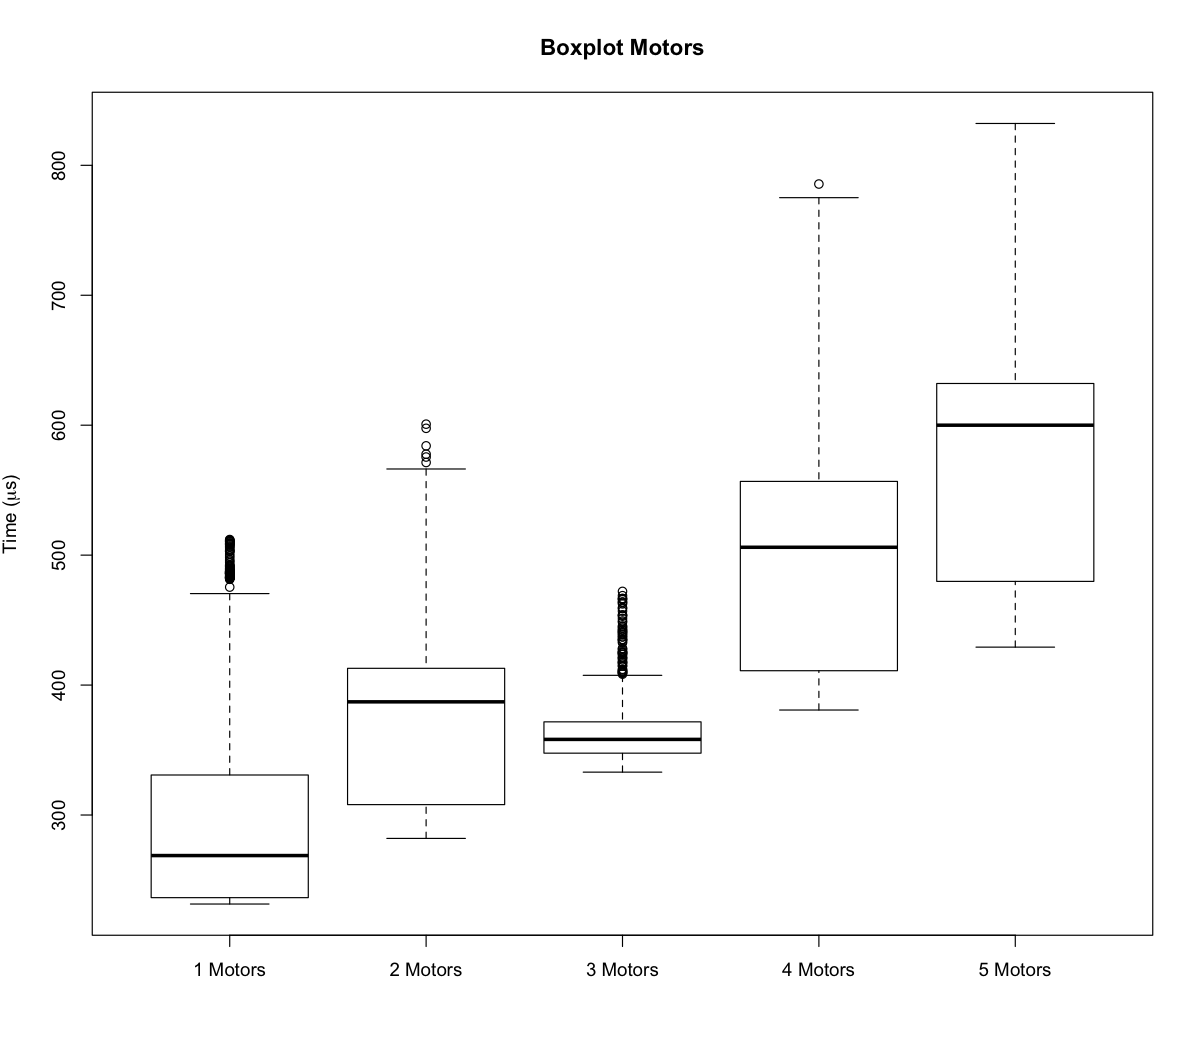
\includegraphics[width=0.8\textwidth]{evaluation/graphics/Xamarin/Galaxy/BoxplotMotorsXamarinGalaxy.png} 
    \caption[Gráficos de cajas de motores Xamarin-Galaxy]{Gráficos de cajas de motores Xamarin-Galaxy\\Fuente: elaboración propia (2018)} 
    \label{fig:xamarin-galaxy-boxplot-motors}
  \end{center}
\end{figure}

\subsubsection{Flexores}
% {START} RESUME TABLE ---------------------------------
%\extracolsep{-11pt}
%\caption[Resumen resultado pruebas flexor Xamarin-Galaxy]{Resumen resultado pruebas flexor Xamarin-Galaxy \\ Fuente: Elaboración propia (2018)}
%\label{table:flexor-xamarin-galaxy}

% Table created by stargazer v.5.2.2 by Marek Hlavac, Harvard University. E-mail: hlavac at fas.harvard.edu
% Date and time: Tue, Jul 03, 2018 - 20:10:45
% Requires LaTeX packages: dcolumn 
\begin{table}[!htbp]
\centering 
\caption[Resumen resultado pruebas flexor Xamarin-Galaxy]{Resumen resultado pruebas flexor Xamarin-Galaxy en $\mu s$\\ Fuente: Elaboración propia (2018)}
\label{table:flexor-xamarin-galaxy}
\begin{tabular}{@{\extracolsep{-11pt}} D{.}{.}{-3} D{.}{.}{-3} D{.}{.}{-3} D{.}{.}{-3} D{.}{.}{-3} D{.}{.}{-3} D{.}{.}{-3} D{.}{.}{-3} } 
\\[-1.8ex]\hline 
\hline \\[-1.8ex] 
\multicolumn{1}{c}{Motors} & \multicolumn{1}{c}{Mean} & \multicolumn{1}{c}{Median} & \multicolumn{1}{c}{Min} & \multicolumn{1}{c}{Max} & \multicolumn{1}{c}{Std. Dev.} & \multicolumn{1}{c}{Skewness} & \multicolumn{1}{c}{Kurtosis} \\ 
\hline \\[-1.8ex] 
1 & 123,483.700 & 109,237.600 & 55,364.200 & 253,747.900 & 39,493.110 & 0.696 & 2.824 \\ 
\hline \\[-1.8ex] 
\end{tabular} 
\end{table} 
% {END} RESUME TABLE ---------------------------------

\begin{figure}
 \begin{center} 
   	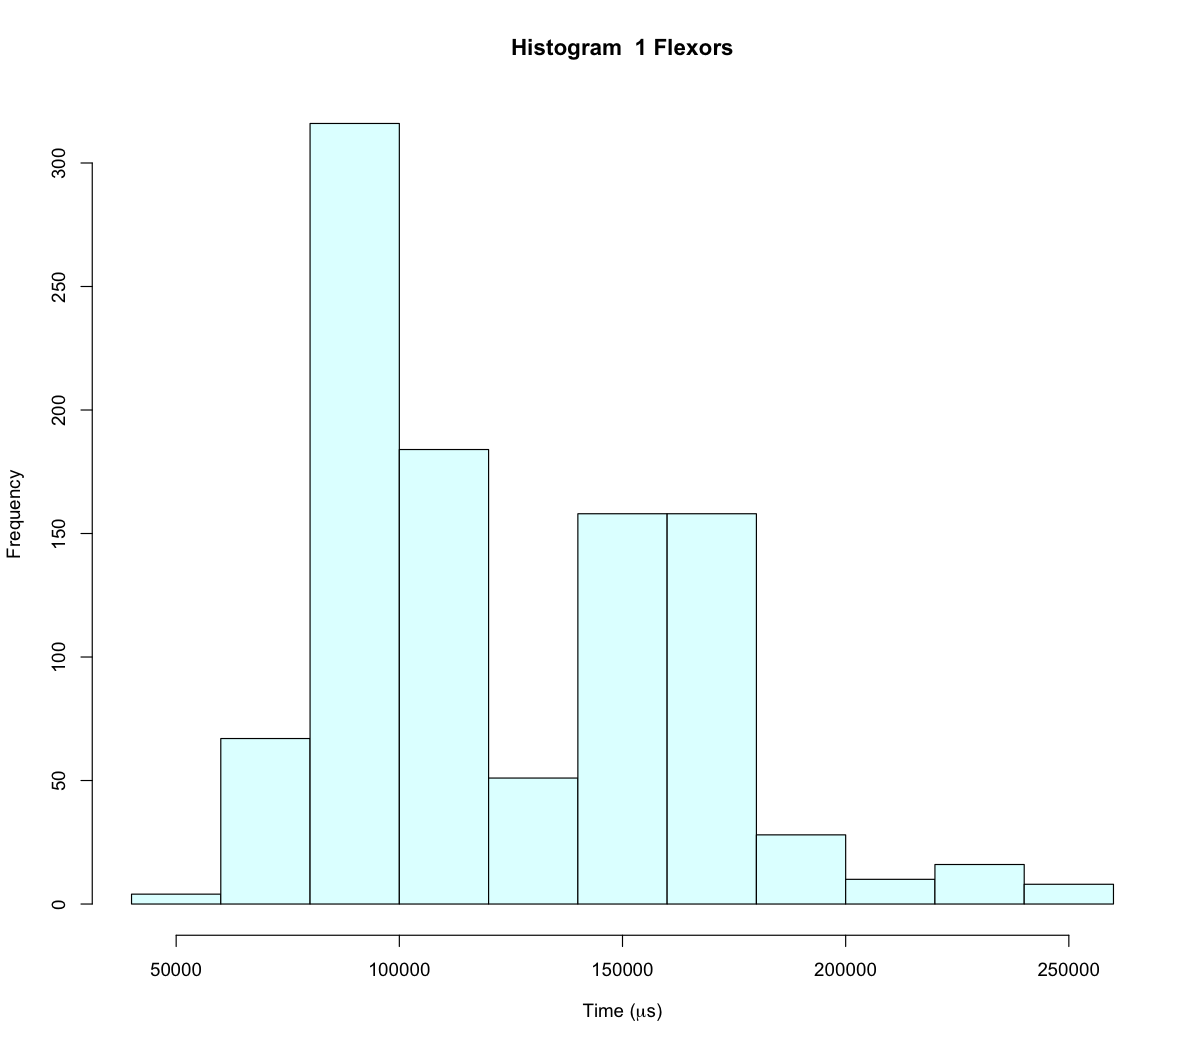
\includegraphics[width=0.5\textwidth]{evaluation/graphics/Xamarin/Galaxy/HistFlexorsXamarinGalaxy.png} 
    \caption[Histogramas de flexores Xamarin-Galaxy]{Histogramas de flexores Xamarin-Galaxy\\Fuente: elaboración propia (2018)} 
    \label{fig:xamarin-galaxy-hist-flexors}
  \end{center}
\end{figure}

\begin{figure}[H]
  \begin{center} 
   	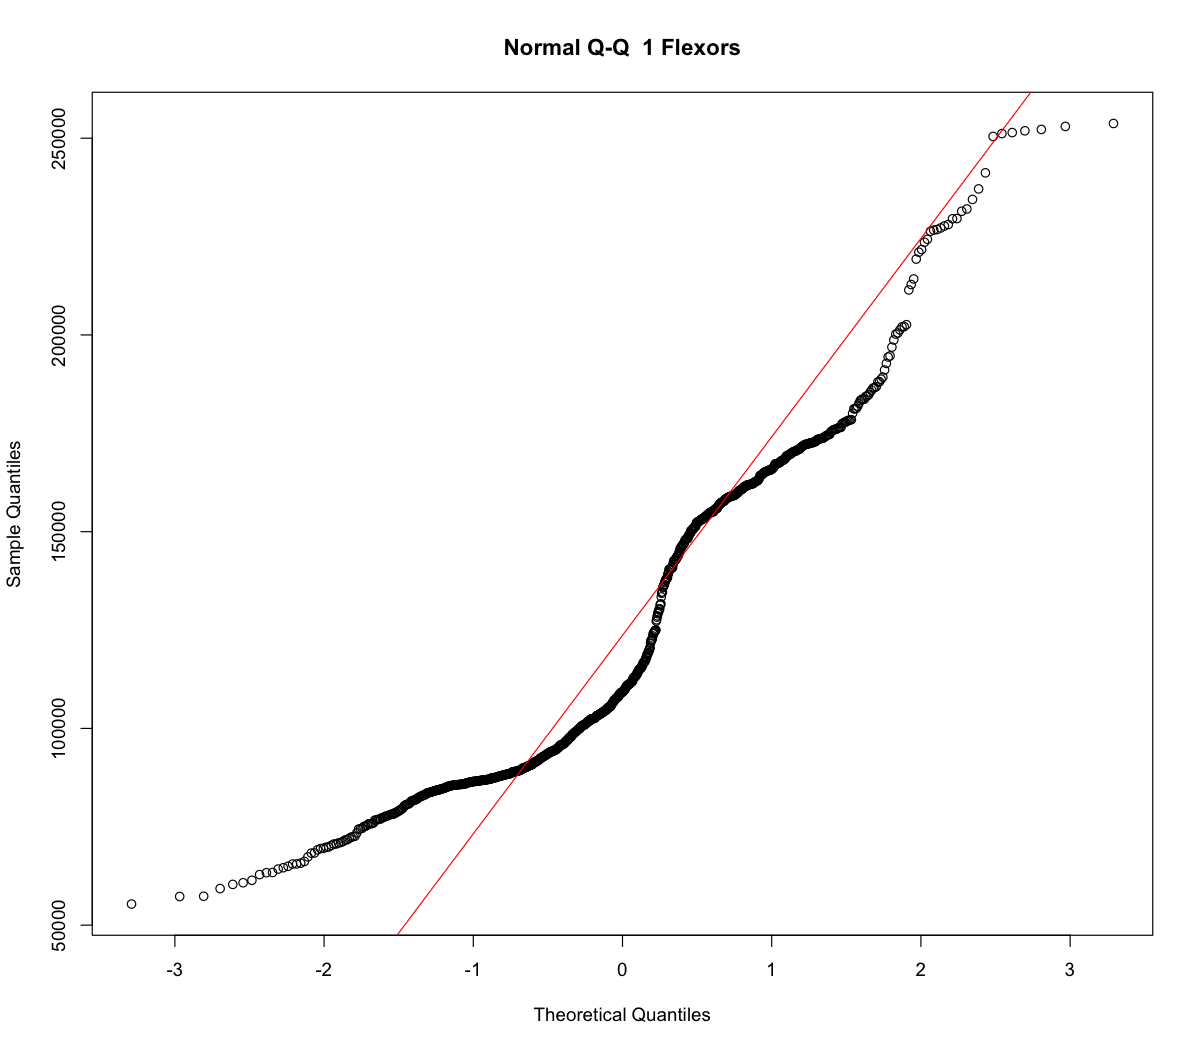
\includegraphics[width=0.5\textwidth]{evaluation/graphics/Xamarin/Galaxy/NormalQQFlexorsXamarinGalaxy.png} 
    \caption[Gráfico QQ de flexores Xamarin-Galaxy]{Gráficos QQ de flexores Xamarin-Galaxy\\Fuente: elaboración propia (2018)} 
    \label{fig:xamarin-galaxy-QQ-flexors}
  \end{center}
\end{figure}

\begin{figure}[H]
  \begin{center} 
   	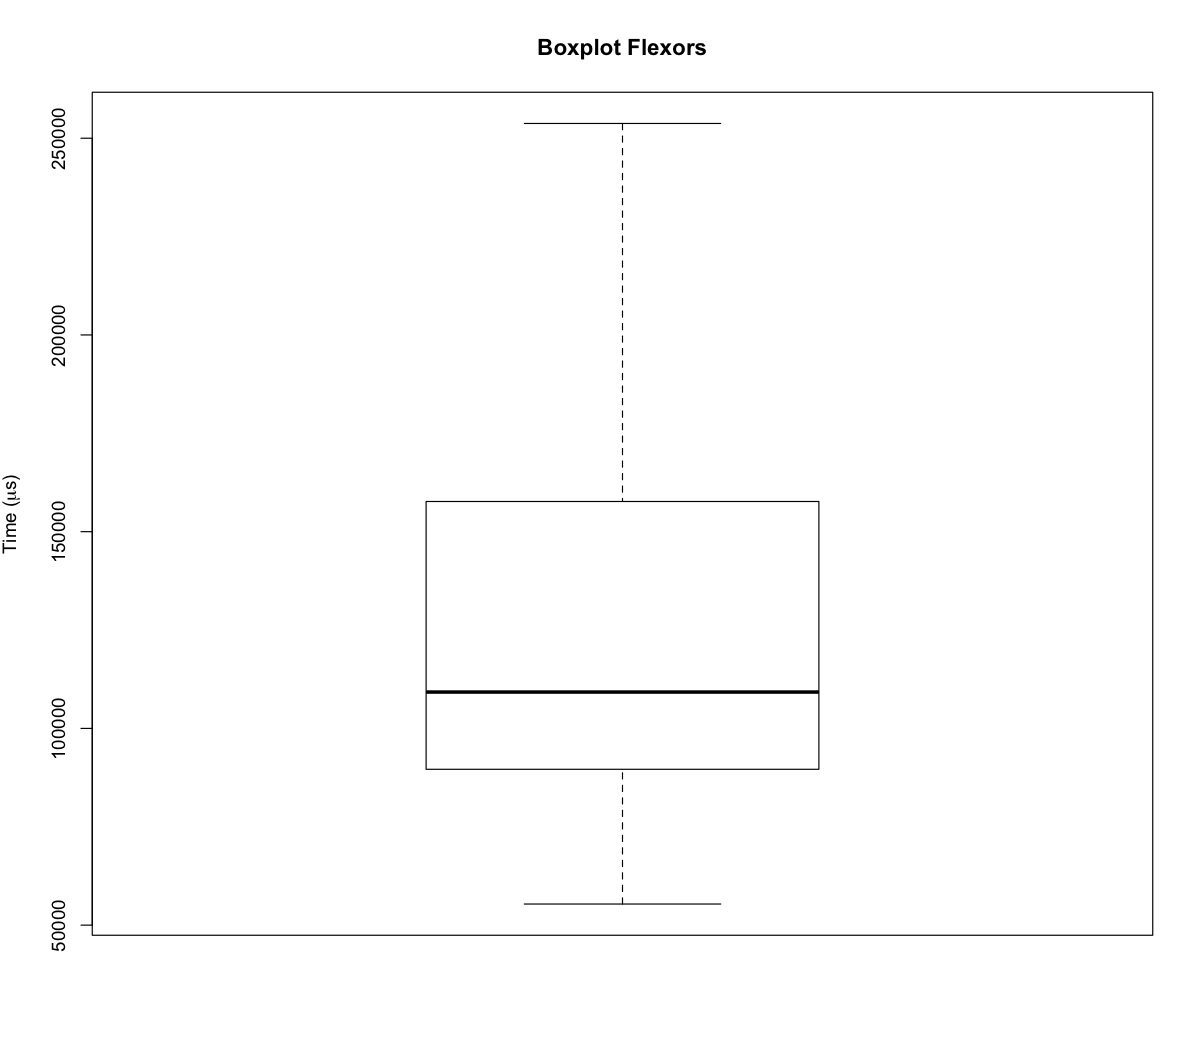
\includegraphics[width=0.5\textwidth]{evaluation/graphics/Xamarin/Galaxy/BoxplotFlexorsXamarinGalaxy.png} 
    \caption[Gráficos de cajas de flexores Xamarin-Galaxy]{Gráficos de cajas de flexores Xamarin-Galaxy\\Fuente: elaboración propia (2018)} 
    \label{fig:xamarin-galaxy-boxplot-flexors}
  \end{center}
\end{figure}



\subsection{Prototipo 3 : Droid - Nexus}

\subsubsection{Motores}
% {START} RESUME TABLE ---------------------------------
%\caption[Resumen resultado pruebas motor Droid-Nexus]{Resumen resultado pruebas motor Droid-Nexus  en $\mu s$\\ Fuente: Elaboración propia (2018)}
%\label{table:motor-droid-nexus} 

% Table created by stargazer v.5.2.2 by Marek Hlavac, Harvard University. E-mail: hlavac at fas.harvard.edu
% Date and time: Tue, Jul 03, 2018 - 19:28:30
% Requires LaTeX packages: dcolumn 
% Table created by stargazer v.5.2.2 by Marek Hlavac, Harvard University. E-mail: hlavac at fas.harvard.edu
% Date and time: Mon, Sep 03, 2018 - 17:49:12
\begin{table}[!htbp] \centering 
\caption[Resumen resultado pruebas motor Droid-Nexus]{Resumen resultado pruebas motor Droid-Nexus  en $\mu s$\\ Fuente: Elaboración propia (2018)}
\label{table:motor-droid-nexus} 
\begin{tabular}{@{\extracolsep{5pt}} cccccccc} 
\\[-1.8ex]\hline 
\hline \\[-1.8ex] 
motors & Mean & Median & Min & Max & Std. Dev. & Skewness & Kurtosis \\ 
\hline \\[-1.8ex] 
$1$ & $187.574$ & $171.979$ & $133.646$ & $335.416$ & $44.577$ & $0.337$ & $1.905$ \\ 
$2$ & $231.251$ & $192.761$ & $168.230$ & $482.136$ & $63.706$ & $0.773$ & $2.835$ \\ 
$3$ & $237.638$ & $220.105$ & $202.812$ & $387.813$ & $44.517$ & $1.965$ & $5.687$ \\ 
$4$ & $262.838$ & $258.646$ & $240.938$ & $391.615$ & $20.442$ & $2.567$ & $13.078$ \\ 
$5$ & $336.917$ & $301.250$ & $276.667$ & $592.553$ & $79.910$ & $1.566$ & $3.872$ \\ 
\hline \\[-1.8ex] 
\end{tabular} 
\end{table} 
% {END} RESUME TABLE ---------------------------------

La Figura \ref{fig:droid-nexus-hist-motors}, muestra los histogramas de las latencias obtenidas al mandar los mensajes de activación y desactivación. Se realizaron pruebas desde uno a cinco motores.

\begin{figure}
 \begin{center} 
   	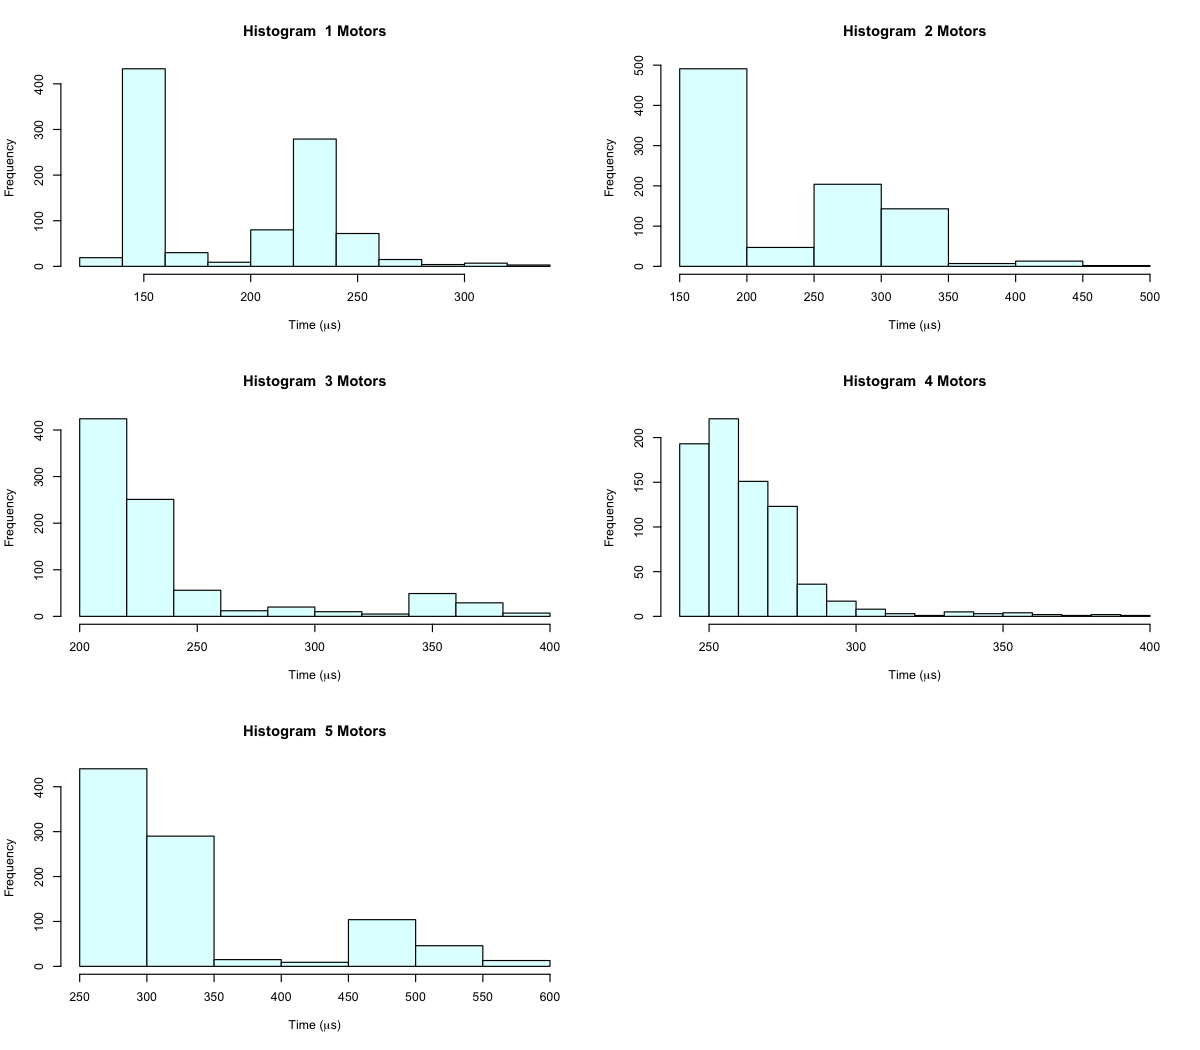
\includegraphics[width=1.0\textwidth]{evaluation/graphics/Droid/Nexus/HistMotorsDroidNexus.png} 
    \caption[Histogramas de motores Droid-Nexus]{Histogramas de motores  Droid-Nexus\\Fuente: elaboración propia (2018)} 
    \label{fig:droid-nexus-hist-motors}
  \end{center}
\end{figure}

\begin{figure}[H]
  \begin{center} 
   	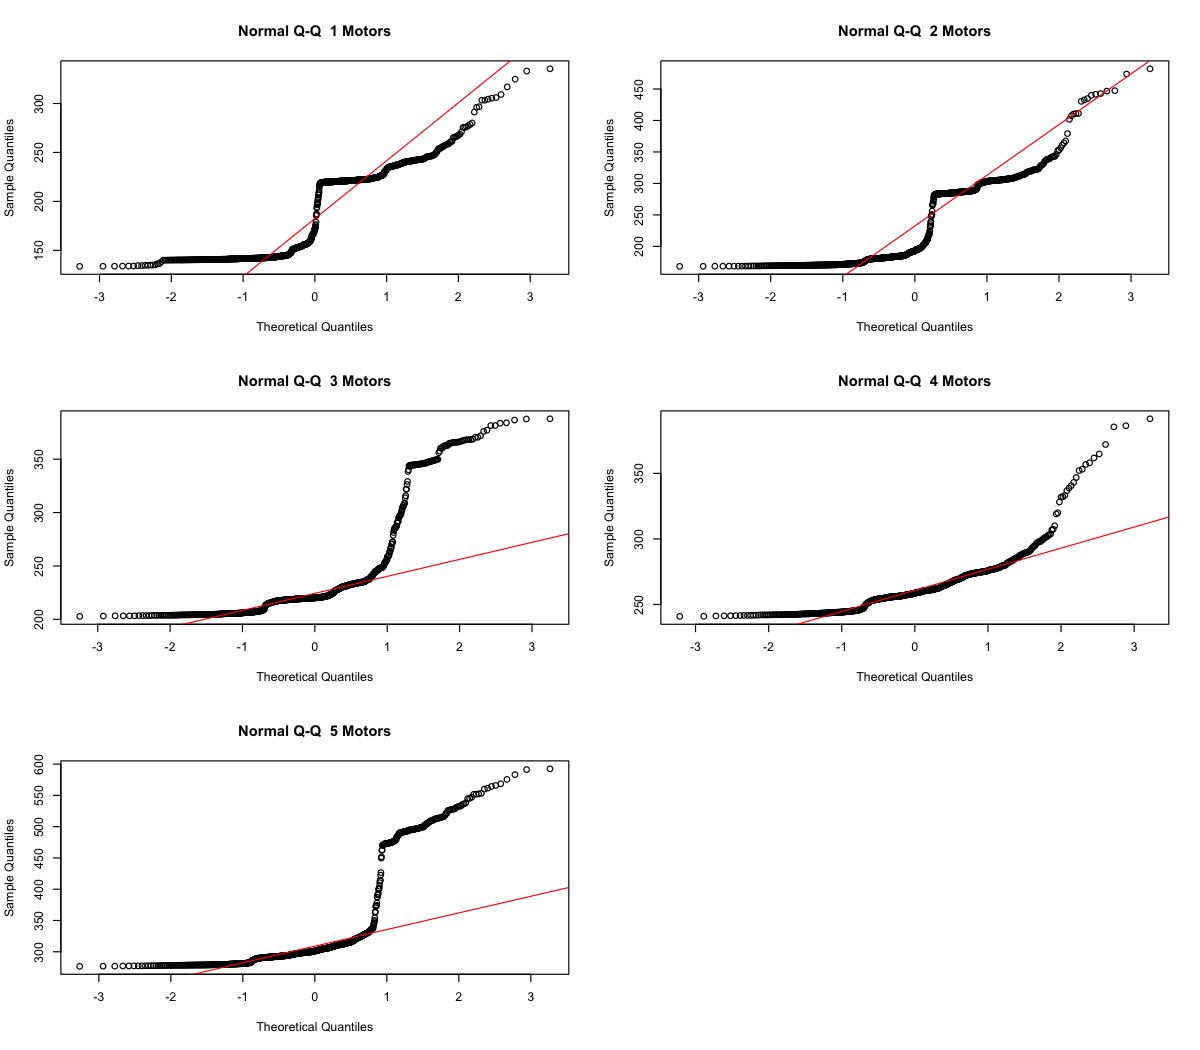
\includegraphics[width=1.0\textwidth]{evaluation/graphics/Droid/Nexus/NormalQQMotorsDroidNexus.png} 
    \caption[Gráfico QQ de motores Droid-Nexus]{Gráficos QQ de motores Droid-Nexus\\Fuente: elaboración propia (2018)} 
    \label{fig:droid-nexus-QQ-motors}
  \end{center}
\end{figure}

\begin{figure}[H]
  \begin{center} 
   	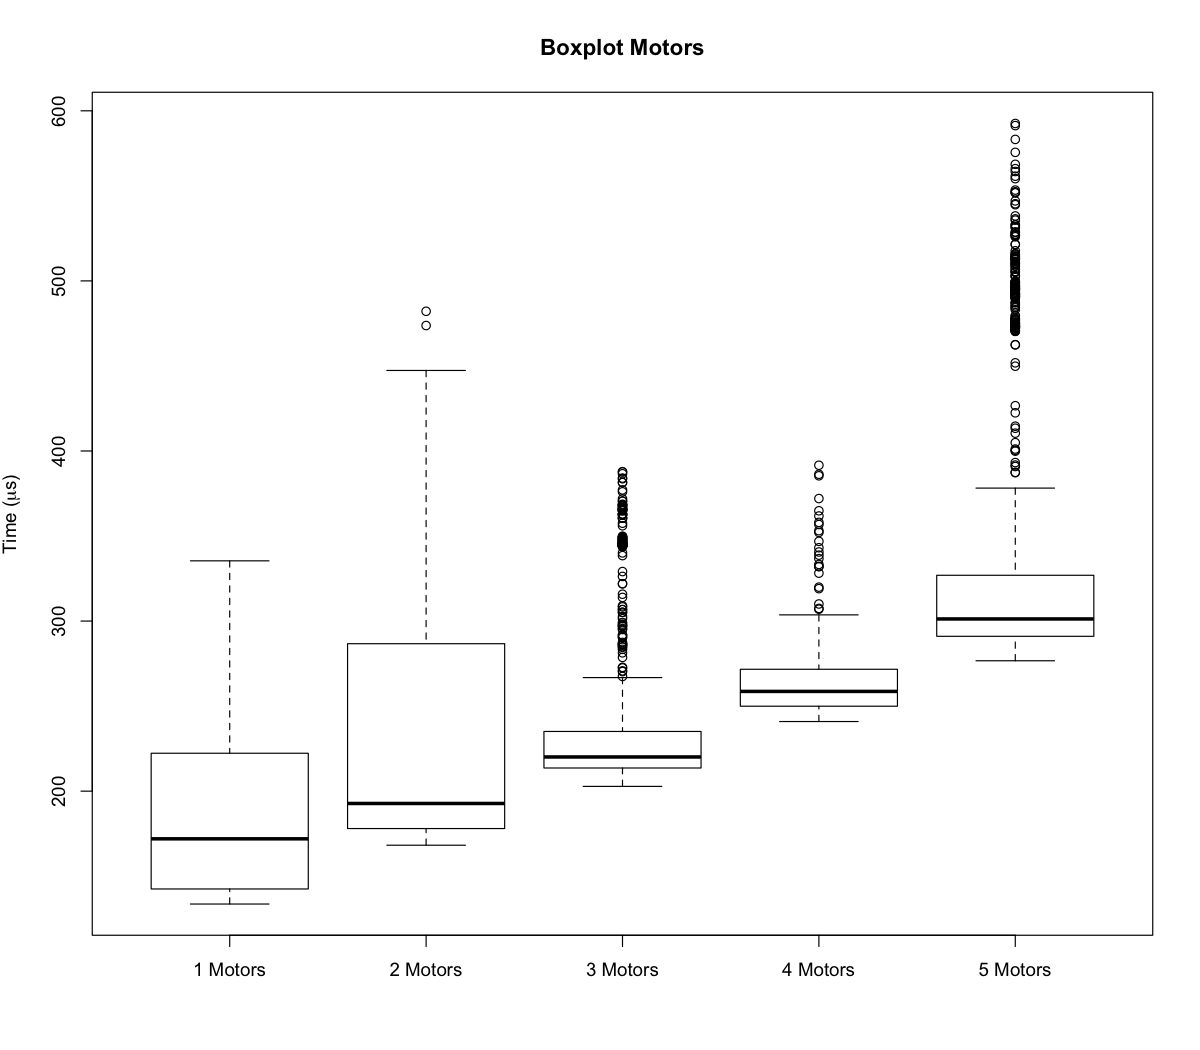
\includegraphics[width=0.8\textwidth]{evaluation/graphics/Droid/Nexus/BoxplotMotorsDroidNexus.png} 
    \caption[Gráficos de cajas de motores Droid-Nexus]{Gráficos de cajas de motores Droid-Nexus\\Fuente: elaboración propia (2018)} 
    \label{fig:droid-nexus-boxplot-motors}
  \end{center}
\end{figure}

\subsubsection{Flexores}
% {START} RESUME TABLE ---------------------------------
%\extracolsep{-11pt}
%\caption[Resumen resultado pruebas flexor Droid-Nexus]{Resumen resultado pruebas flexor Droid-Nexus en $\mu s$\\ Fuente: Elaboración propia (2018)}
%\label{table:flexor-droid-nexus}

% Table created by stargazer v.5.2.2 by Marek Hlavac, Harvard University. E-mail: hlavac at fas.harvard.edu
% Date and time: Mon, Sep 03, 2018 - 17:53:15
\begin{table}[!htbp] \centering 
\caption[Resumen resultado pruebas flexor Droid-Nexus]{Resumen resultado pruebas flexor Droid-Nexus en $\mu s$ \\ Fuente: Elaboración propia (2018)}
\label{table:flexor-droid-nexus}
\begin{tabular}{@{\extracolsep{5pt}} cccccccc} 
\\[-1.8ex]\hline 
\hline \\[-1.8ex] 
flexors & Mean & Median & Min & Max & Std. Dev. & Skewness & Kurtosis \\ 
\hline \\[-1.8ex] 
$1$ & $109,671$ & $114,496$ & $48,099.480$ & $172,982.100$ & $24,155.450$ & $-0.304$ & $2.621$ \\ 
\hline \\[-1.8ex] 
\end{tabular} 
\end{table} 
% {END} RESUME TABLE ---------------------------------

\begin{figure}
 \begin{center} 
   	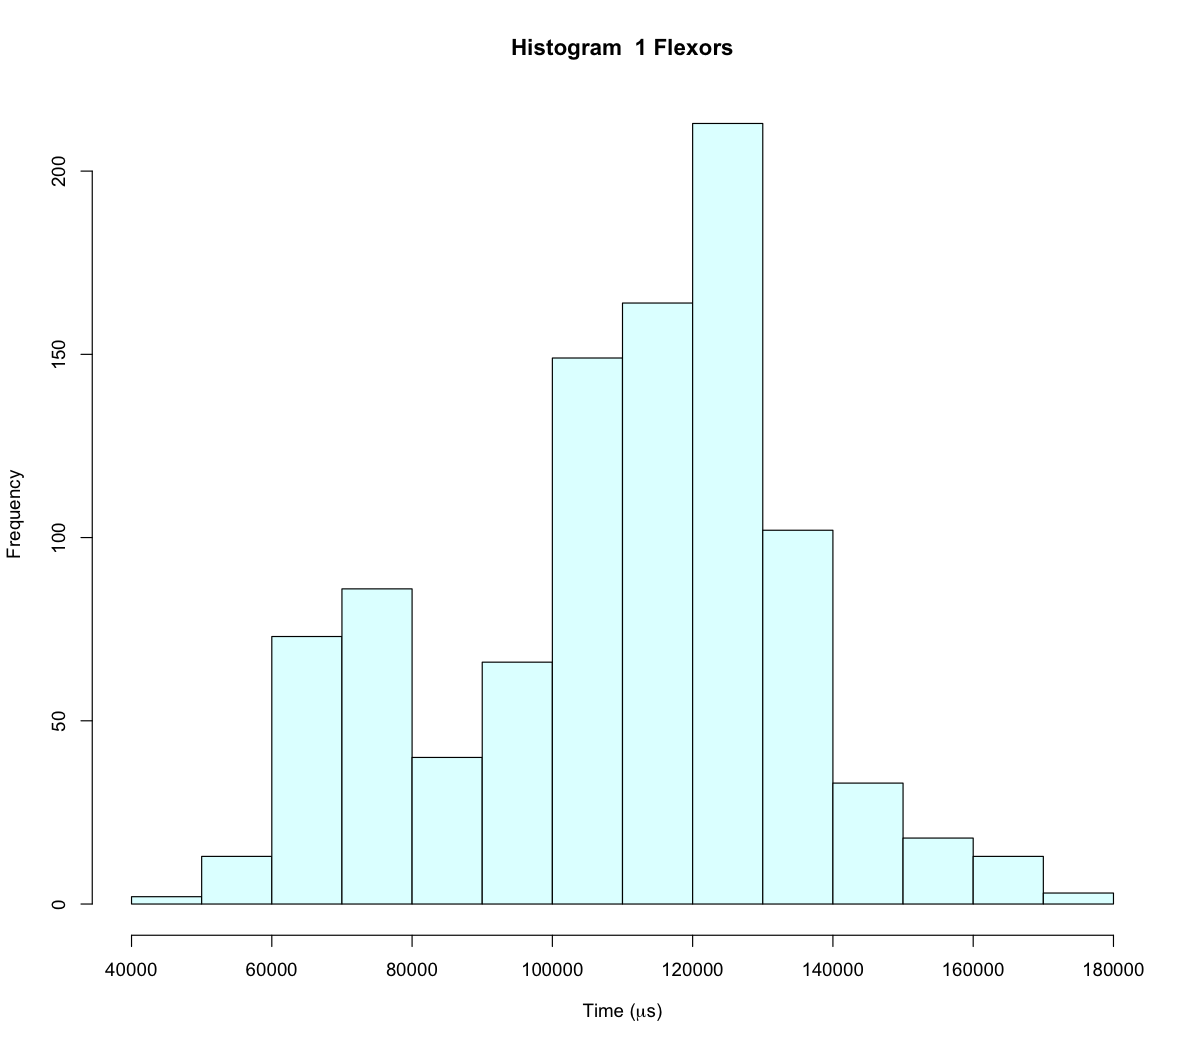
\includegraphics[width=0.5\textwidth]{evaluation/graphics/Droid/Nexus/HistFlexorsDroidNexus.png} 
    \caption[Histogramas de flexores Droid-Nexus]{Histogramas de flexores  Droid-Nexus\\Fuente: elaboración propia (2018)} 
    \label{fig:droid-nexus-hist-flexors}
  \end{center}
\end{figure}

\begin{figure}[H]
  \begin{center} 
   	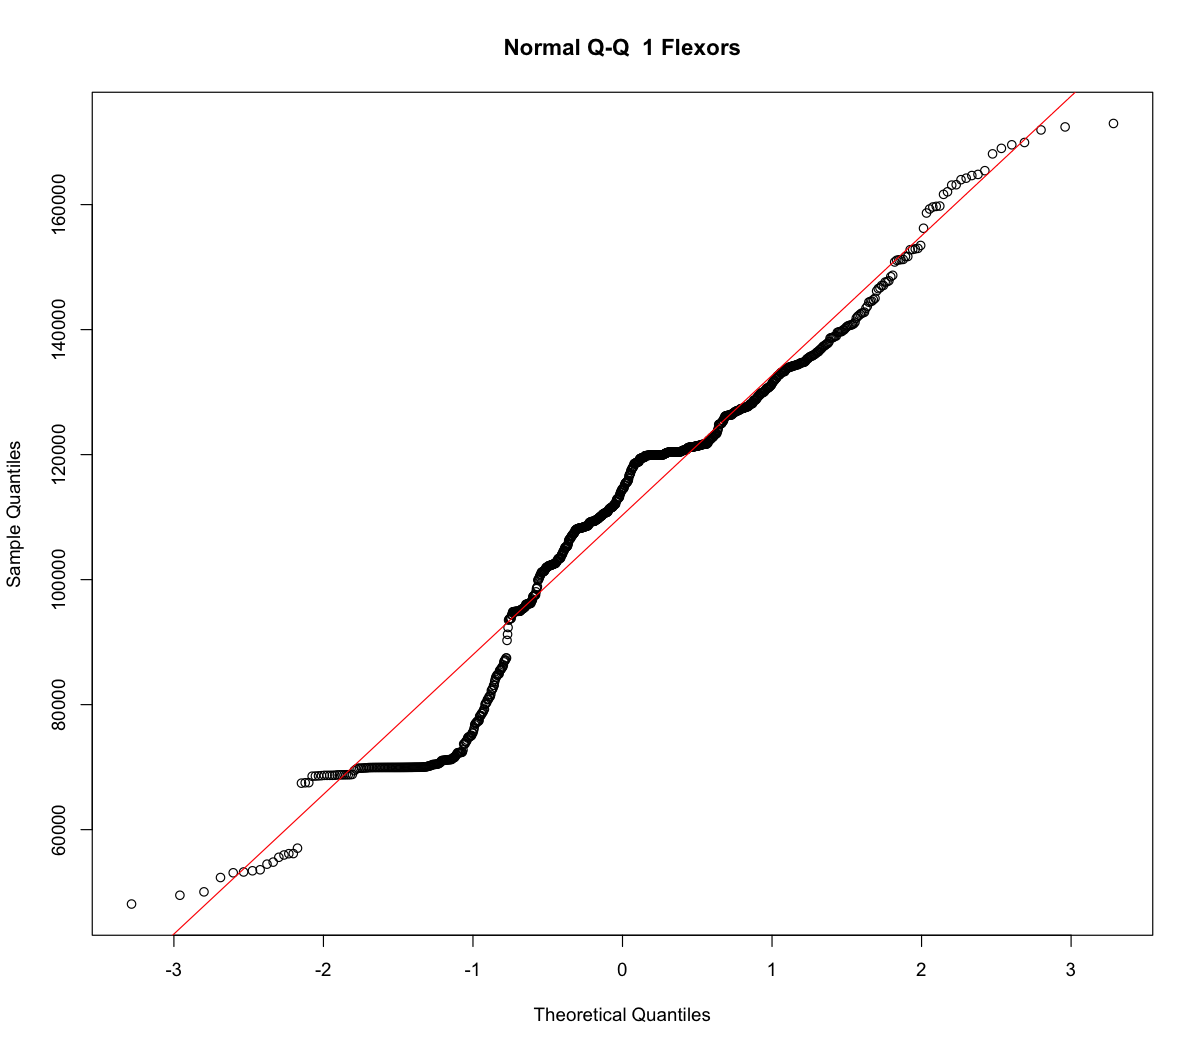
\includegraphics[width=0.5\textwidth]{evaluation/graphics/Droid/Nexus/NormalQQFlexorsDroidNexus.png} 
    \caption[Gráfico QQ de flexores Droid-Nexus]{Gráficos QQ de flexores Droid-Nexus\\Fuente: elaboración propia (2018)} 
    \label{fig:droid-nexus-QQ-flexors}
  \end{center}
\end{figure}

\begin{figure}[H]
  \begin{center} 
   	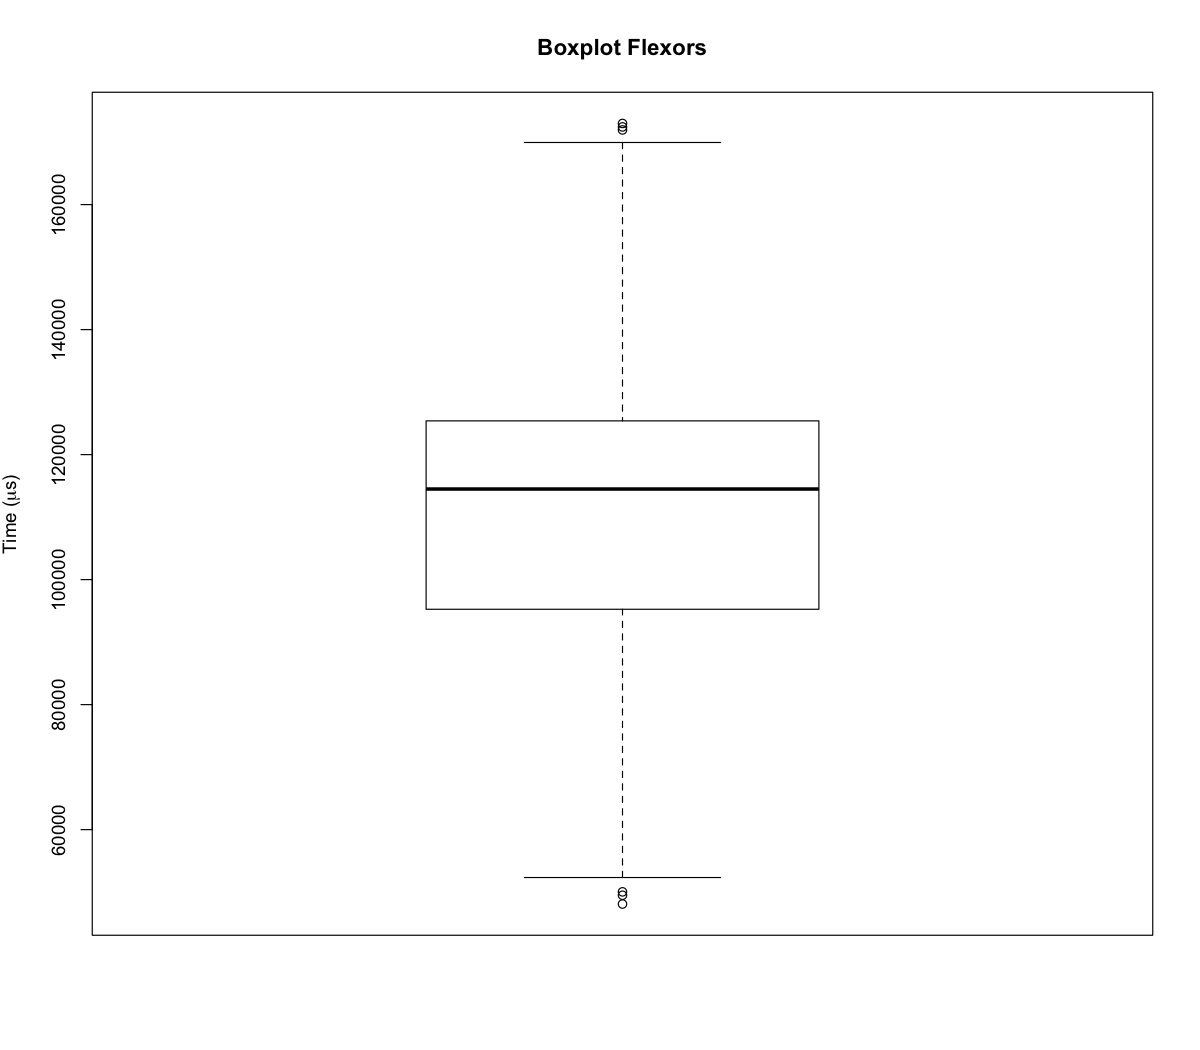
\includegraphics[width=0.5\textwidth]{evaluation/graphics/Droid/Nexus/BoxplotFlexorsDroidNexus.png} 
    \caption[Gráficos de cajas de flexores Droid-Nexus]{Gráficos de cajas de flexores Droid-Nexus\\Fuente: elaboración propia (2018)} 
    \label{fig:droid-nexus-boxplot-flexors}
  \end{center}
\end{figure}

\subsection{Prototipo 4: Xamarin - Nexus}

\subsubsection{Motores}

% {START} RESUME TABLE ---------------------------------
%\caption[Resumen resultado pruebas motor Xamarin-Nexus]{Resumen resultado pruebas motor Xamarin-Nexus  en $\mu s$\\ Fuente: Elaboración propia (2018)}
%\label{table:motor-xamarin-nexus} 

% Table created by stargazer v.5.2.2 by Marek Hlavac, Harvard University. E-mail: hlavac at fas.harvard.edu
% Date and time: Mon, Sep 03, 2018 - 17:56:53
\begin{table}[!htbp] \centering 
\caption[Resumen resultado pruebas motor Xamarin-Nexus]{Resumen resultado pruebas motor Xamarin-Nexus  en $\mu s$\\ Fuente: Elaboración propia (2018)}
\label{table:motor-xamarin-nexus} 
\begin{tabular}{@{\extracolsep{5pt}} cccccccc} 
\\[-1.8ex]\hline 
\hline \\[-1.8ex] 
motors & Mean & Median & Min & Max & Std. Dev. & Skewness & Kurtosis \\ 
\hline \\[-1.8ex] 
$1$ & $206.856$ & $193.600$ & $185.300$ & $288.900$ & $29.516$ & $1.673$ & $4.187$ \\ 
$2$ & $296.004$ & $243.100$ & $225.600$ & $570.200$ & $83.534$ & $0.995$ & $2.558$ \\ 
$3$ & $275.752$ & $275.400$ & $264.100$ & $316.400$ & $8.007$ & $1.078$ & $5.129$ \\ 
$4$ & $309.417$ & $307.950$ & $296.600$ & $333.300$ & $6.822$ & $0.707$ & $3.544$ \\ 
$5$ & $363.526$ & $341.100$ & $328.400$ & $545.300$ & $54.915$ & $2.211$ & $6.235$ \\ 
\hline \\[-1.8ex] 
\end{tabular} 
\end{table} 
% {END} RESUME TABLE ---------------------------------

La Figura \ref{fig:xamarin-nexus-hist-motors}, muestra los histogramas de las latencias obtenidas al mandar los mensajes de activación y desactivación. Se realizaron pruebas desde uno a cinco motores.

\begin{figure}
 \begin{center} 
   	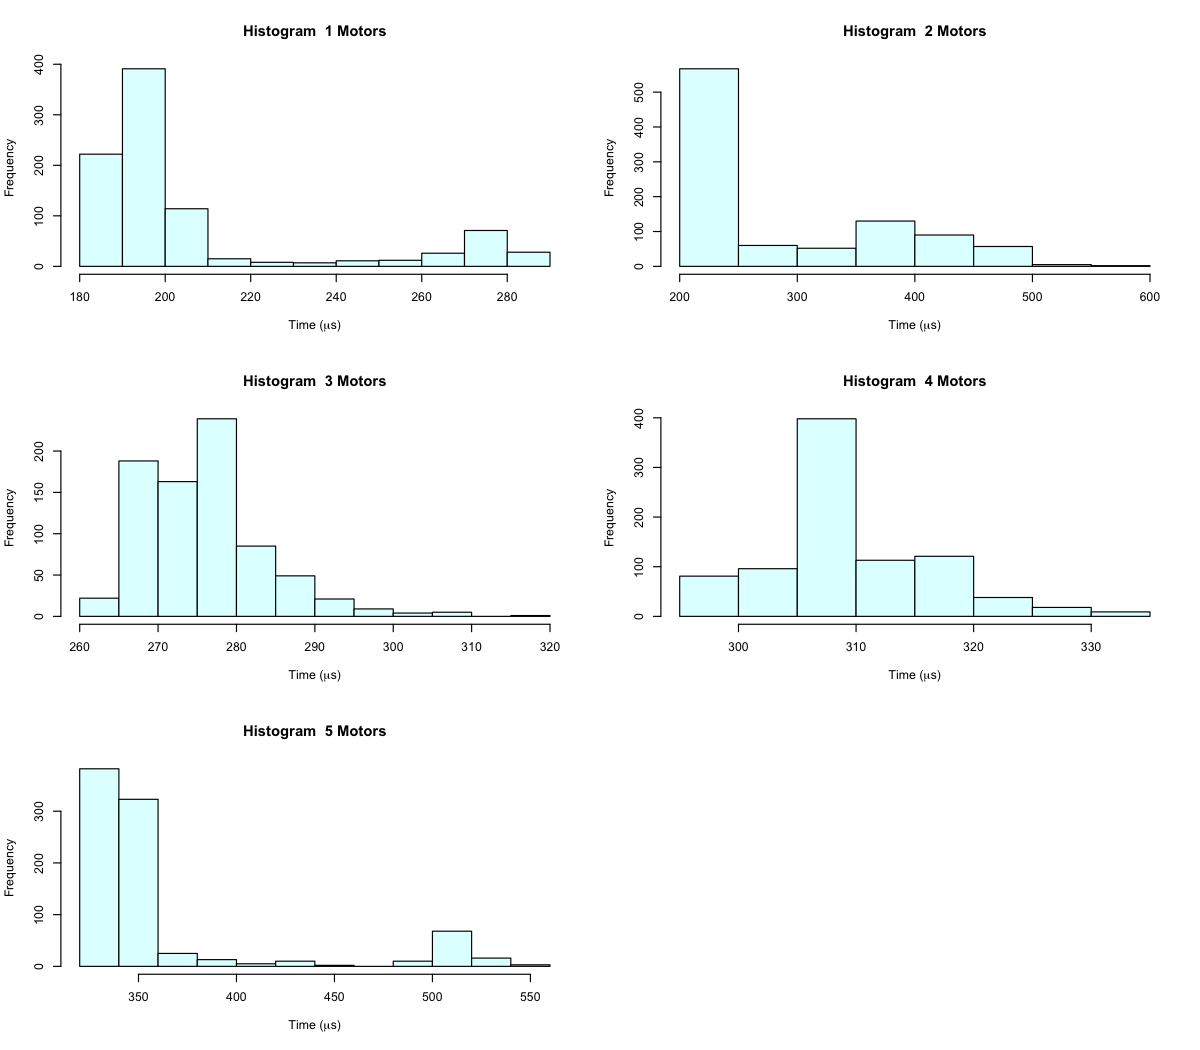
\includegraphics[width=1.0\textwidth]{evaluation/graphics/Xamarin/Nexus/HistMotorsXamarinNexus.png} 
    \caption[Histogramas de motores Xamarin-Nexus]{Histogramas de motores  Xamarin-Nexus\\Fuente: elaboración propia (2018)} 
    \label{fig:xamarin-nexus-hist-motors}
  \end{center}
\end{figure}

\begin{figure}[H]
  \begin{center} 
   	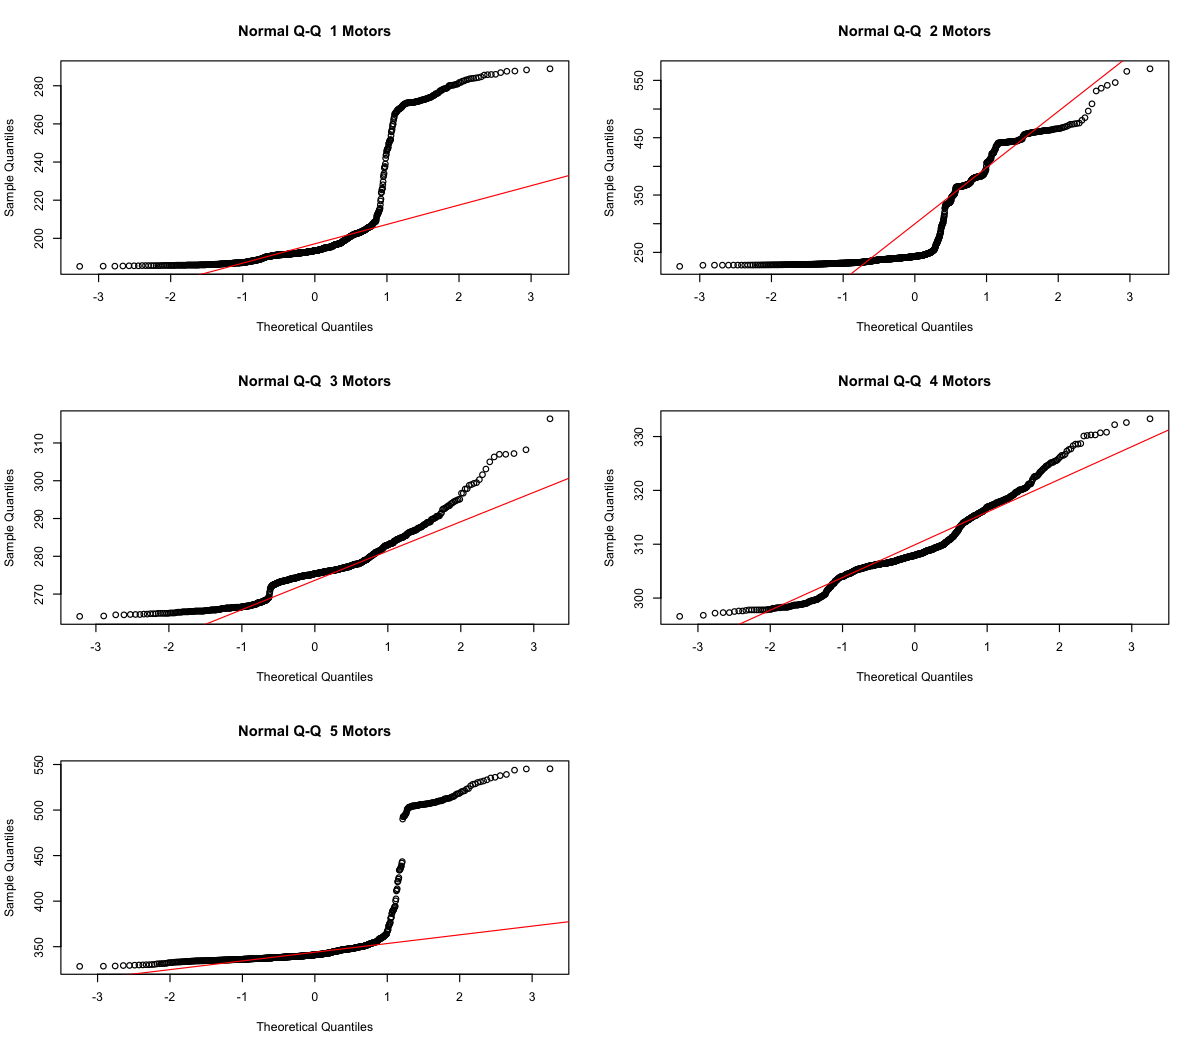
\includegraphics[width=1.0\textwidth]{evaluation/graphics/Xamarin/Nexus/NormalQQMotorsXamarinNexus.png} 
    \caption[Gráfico QQ de motores Xamarin-Nexus]{Gráficos QQ de motores Xamarin-Nexus\\Fuente: elaboración propia (2018)} 
    \label{fig:xamarin-nexus-QQ-motors}
  \end{center}
\end{figure}

\begin{figure}[H]
  \begin{center} 
   	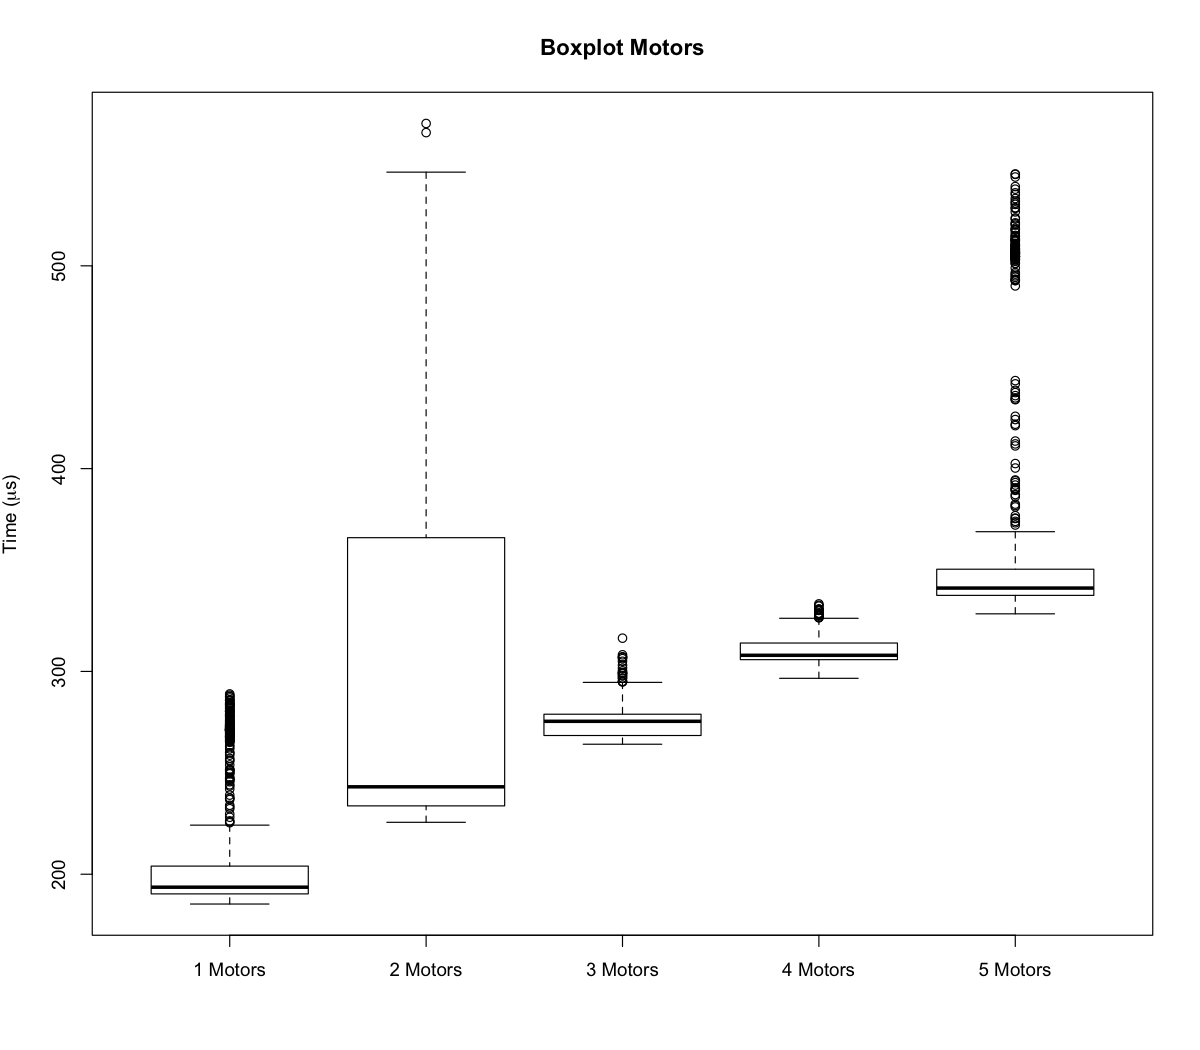
\includegraphics[width=0.8\textwidth]{evaluation/graphics/Xamarin/Nexus/BoxplotMotorsXamarinNexus.png} 
    \caption[Gráficos de cajas de motores Xamarin-Nexus]{Gráficos de cajas de motores Xamarin-Nexus\\Fuente: elaboración propia (2018)} 
    \label{fig:xamarin-nexus-boxplot-motors}
  \end{center}
\end{figure}


\subsubsection{Flexores}

% {START} RESUME TABLE ---------------------------------
%\extracolsep{-11pt}
%\caption[Resumen resultado pruebas flexor Xamarin-Nexus]{Resumen resultado pruebas flexor Xamarin-Nexus en $\mu s$ \\ Fuente: Elaboración propia (2018)}
%\label{table:flexor-xamarin-nexus}

% Table created by stargazer v.5.2.2 by Marek Hlavac, Harvard University. E-mail: hlavac at fas.harvard.edu
% Date and time: Mon, Sep 03, 2018 - 18:04:31
\begin{table}[!htbp] \centering 
\caption[Resumen resultado pruebas flexor Xamarin-Nexus]{Resumen resultado pruebas flexor Xamarin-Nexus en $\mu s$ \\ Fuente: Elaboración propia (2018)}
\label{table:flexor-xamarin-nexus}
\begin{tabular}{@{\extracolsep{5pt}} cccccccc} 
\\[-1.8ex]\hline 
\hline \\[-1.8ex] 
flexors & Mean & Median & Min & Max & Std. Dev. & Skewness & Kurtosis \\ 
\hline \\[-1.8ex] 
$1$ & $109,677$ & $110,958$ & $67,022.400$ & $158,703.500$ & $18,411.270$ & $-0.353$ & $2.914$ \\ 
\hline \\[-1.8ex] 
\end{tabular} 
\end{table} 
% {END} RESUME TABLE ---------------------------------

\begin{figure}
 \begin{center} 
   	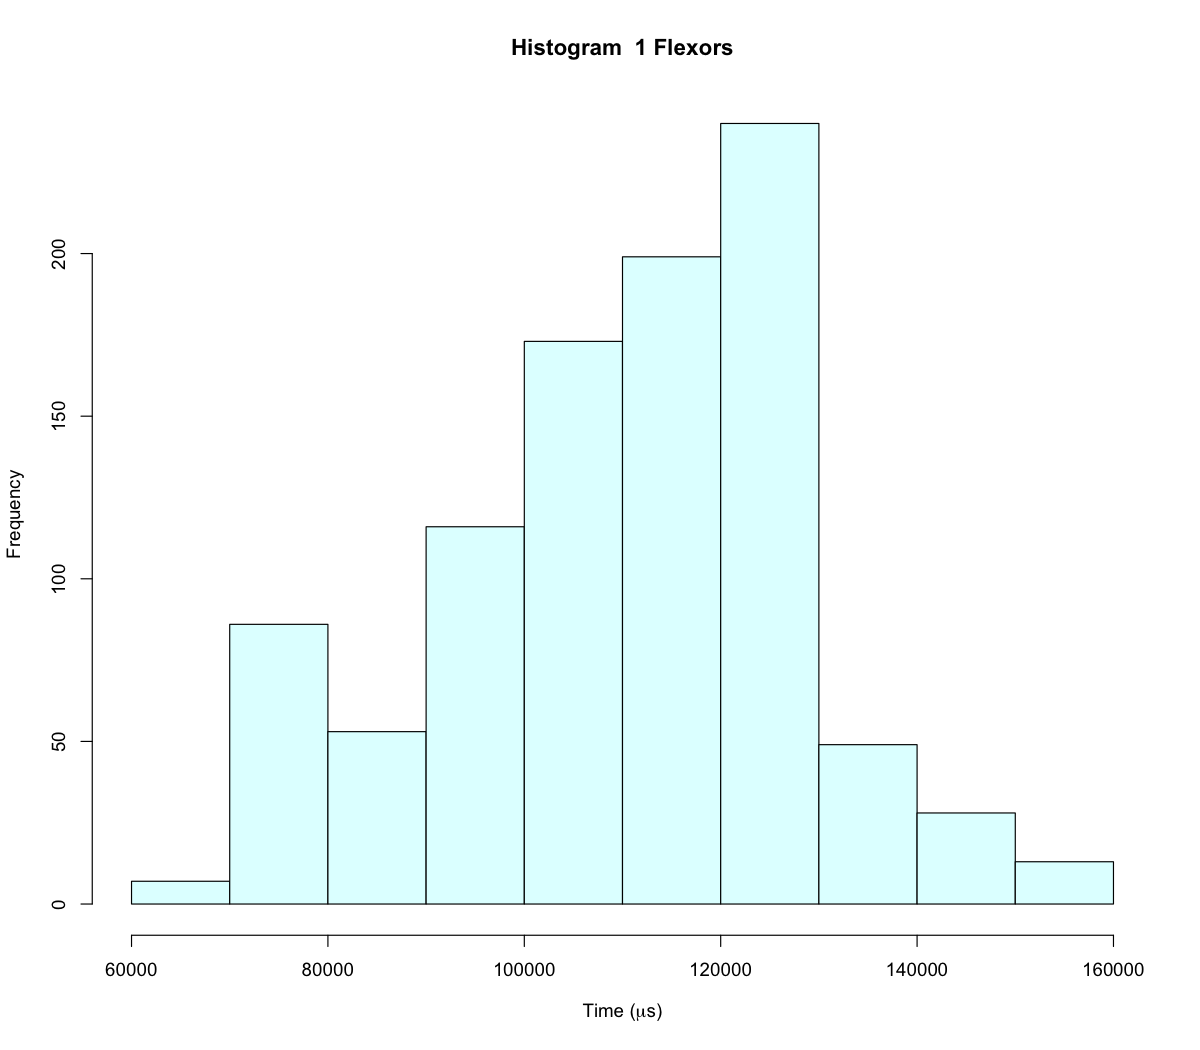
\includegraphics[width=0.5\textwidth]{evaluation/graphics/Xamarin/Nexus/HistFlexorsXamarinNexus.png} 
    \caption[Histogramas de flexores Xamarin-Nexus]{Histogramas de flexores  Xamarin-Nexus\\Fuente: elaboración propia (2018)} 
    \label{fig:xamarin-nexus-hist-flexors}
  \end{center}
\end{figure}

\begin{figure}[H]
  \begin{center} 
   	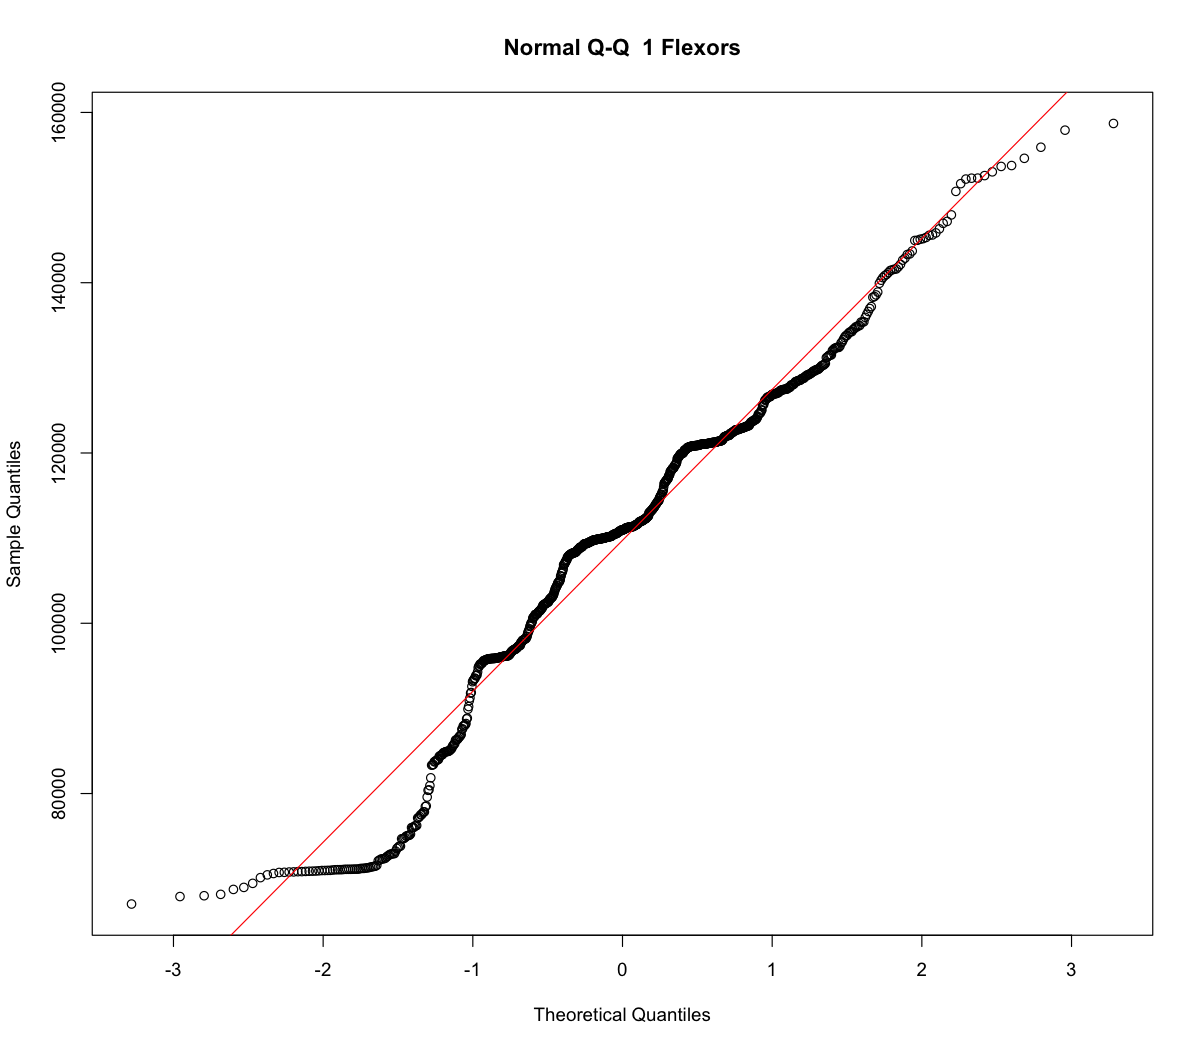
\includegraphics[width=0.5\textwidth]{evaluation/graphics/Xamarin/Nexus/NormalQQFlexorsXamarinNexus.png} 
    \caption[Gráfico QQ de flexores Xamarin-Nexus]{Gráficos QQ de flexores Xamarin-Nexus\\Fuente: elaboración propia (2018)} 
    \label{fig:xamarin-nexus-QQ-flexors}
  \end{center}
\end{figure}

\begin{figure}[H]
  \begin{center} 
   	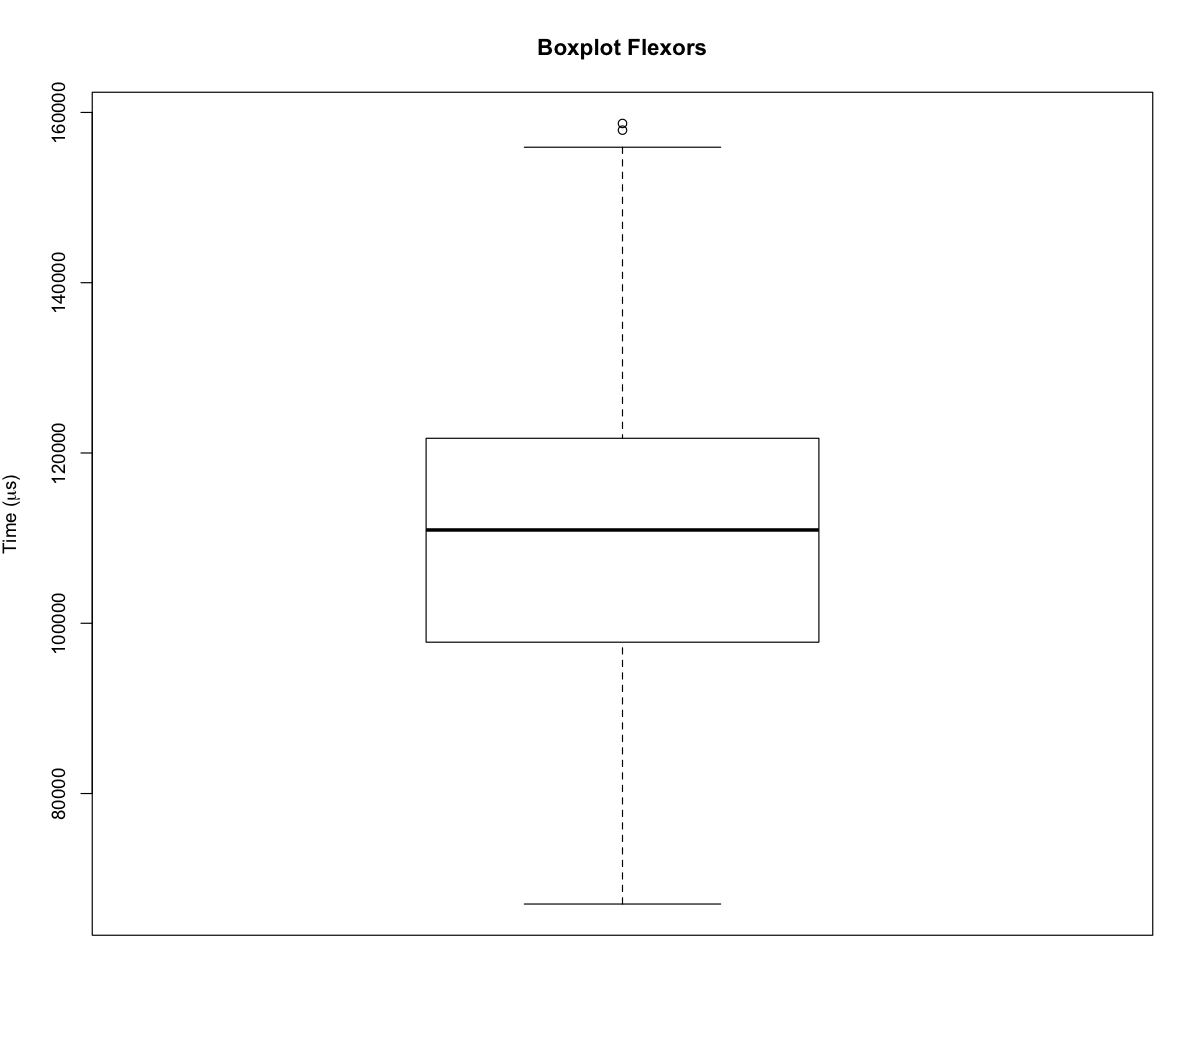
\includegraphics[width=0.5\textwidth]{evaluation/graphics/Xamarin/Nexus/BoxplotFlexorsXamarinNexus.png} 
    \caption[Gráficos de cajas de flexores Xamarin-Nexus]{Gráficos de cajas de flexores Xamarin-Nexus\\Fuente: elaboración propia (2018)} 
    \label{fig:xamarin-nexus-boxplot-flexors}
  \end{center}
\end{figure}

	\section{Evaluación tiempo de activación}

\subsection{API C\#}

\subsection{API Java}
	\section{Evaluación tiempo de lectura de datos usando APIs}
El tipo de prueba que se realizó es el mismo que el utilizado por \cite{tesis-cerda-rodrigo}, por tanto se considera como ciclo de lectura cuando el software de control Arduino, envía los valores de todos los flexores agregados, esto es realizado en paralelo a la lectura de todos los datos que entrega el IMU. Cada medición considera el tiempo transcurrido desde la generación del mensaje en el software de control hasta que llega a la API de alto nivel. Se realizaron 1000 pruebas de ciclos lectura utilizando un Baudrate de 57600, un LoopDelay igual a 0 ms y Threshold igual a 0 en la placa Arduino. Se realizaron pruebas con el IMU enviando la información completa (acelerómetro, giroscopio y magnetómetro) y modificando la cantidad de flexores desde uno a 1 a 10, siendo simulados solamente con un flexor físico en la placa. El dispositivo utilizado para la evaluación técnica de las APIs fue el Samsung Galaxy S5 Mini.

\subsection{API C\#}
%Flexores e IMU update resources

% {START} RESUME TABLE ---------------------------------
%\caption[Resumen resultado pruebas de lectura flexores e IMU usando API C\# ]{Resumen resultado pruebas de lectura flexores e IMU usando API C\#  en $\mu s$\\ Fuente: Elaboración propia (2018)}
%\label{table:flexors&imu-xamarin-galaxy-api}

% Table created by stargazer v.5.2.2 by Marek Hlavac, Harvard University. E-mail: hlavac at fas.harvard.edu
% Date and time: Tue, Sep 04, 2018 - 17:29:17
\begin{table}[!htbp] \centering 
\caption[Resumen resultados de pruebas de lectura flexores e IMU usando API C\#]{Resumen resultados de pruebas de lectura flexores e IMU usando API C\# en $\mu s$\\ Fuente: Elaboración propia (2018)}
\label{table:flexors&imu-xamarin-galaxy-api}
\begin{tabular}{@{\extracolsep{5pt}} cccccccc} 
\\[-1.8ex]\hline 
\hline \\[-1.8ex] 
flexors & Mean & Median & Min & Max & Std. Dev. & Skewness & Kurtosis \\ 
 & $\mu s$ & $\mu s$ & $\mu s$ & $\mu s$ & $\mu s$ &     & \\ 
\hline \\[-1.8ex] 
$1$ & $16,038.830$ & $15,068.100$ & $7,417.900$ & $28,865.600$ & $4,484.658$ & $0.692$ & $2.908$ \\ 
$2$ & $1,365.986$ & $1,271.700$ & $376.800$ & $3,635.400$ & $704.429$ & $0.816$ & $3.307$ \\ 
$3$ & $3,133.853$ & $2,734.500$ & $895.200$ & $8,272.900$ & $1,636.889$ & $1.166$ & $3.906$ \\ 
$4$ & $5,251.955$ & $4,796.100$ & $1,605$ & $12,720.200$ & $2,327.944$ & $0.877$ & $3.417$ \\ 
$5$ & $7,391.620$ & $6,823.100$ & $2,496.400$ & $16,335.200$ & $2,972.165$ & $0.739$ & $3.123$ \\ 
$6$ & $9,445.057$ & $8,723.800$ & $3,565$ & $20,047.800$ & $3,703.347$ & $0.815$ & $3.074$ \\ 
$7$ & $11,231.080$ & $10,768.700$ & $4,948.100$ & $21,445.900$ & $3,611.584$ & $0.609$ & $2.891$ \\ 
$8$ & $12,864.060$ & $12,476.600$ & $6,264.900$ & $24,091.800$ & $3,660.714$ & $0.646$ & $3.045$ \\ 
$9$ & $14,512.320$ & $14,120.300$ & $7,632.200$ & $27,282$ & $4,010.673$ & $0.657$ & $2.891$ \\ 
$10$ & $15,967.690$ & $15,187.800$ & $9,808$ & $27,444.800$ & $3,769.420$ & $0.806$ & $3.086$ \\ 
\hline \\[-1.8ex] 
\end{tabular} 
\end{table} 
% {END} RESUME TABLE ---------------------------------

La Figura \ref{fig:xamarin-galaxy-hist-flexor&imu-api}, muestra los histogramas de las latencias obtenidas al recibir los mensajes de los flexores e IMU, modificando la cantidad de flexores de uno a diez.

\begin{figure}
 \begin{center} 
   	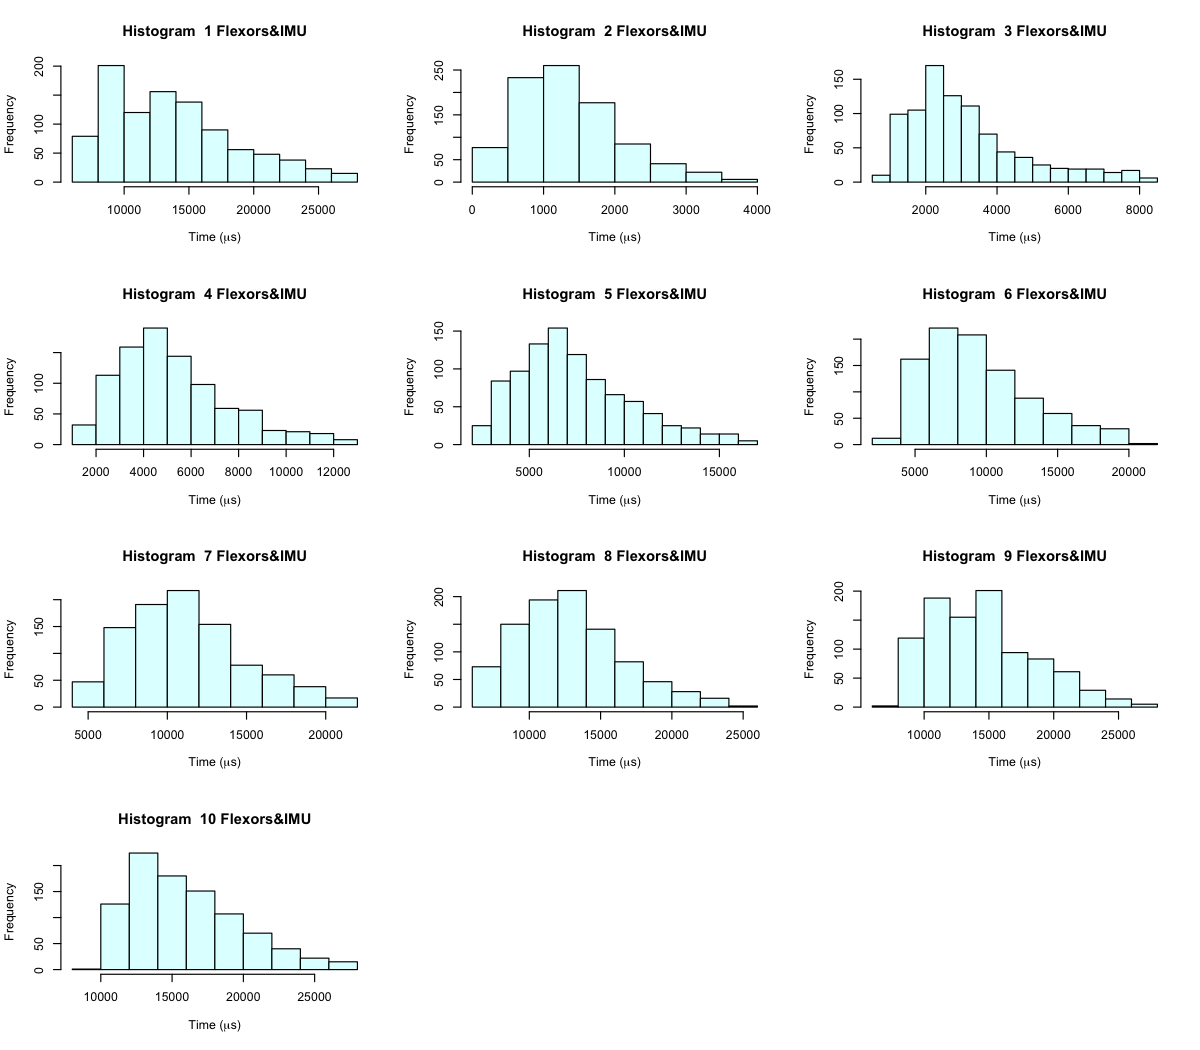
\includegraphics[width=1.0\textwidth]{evaluation/graphics/Xamarin/Galaxy-APITest/HistFlexors&IMUXamarinGalaxy-APITest.png}
   \centering
    \caption[Histogramas de Flexores e IMU usando API C\#]{Histogramas de Flexores e IMU usando API C\# \\Fuente: elaboración propia (2018)}
    \label{fig:xamarin-galaxy-hist-flexors&imu-api}
  \end{center}
\end{figure}

\begin{figure}[H]
  \begin{center} 
   	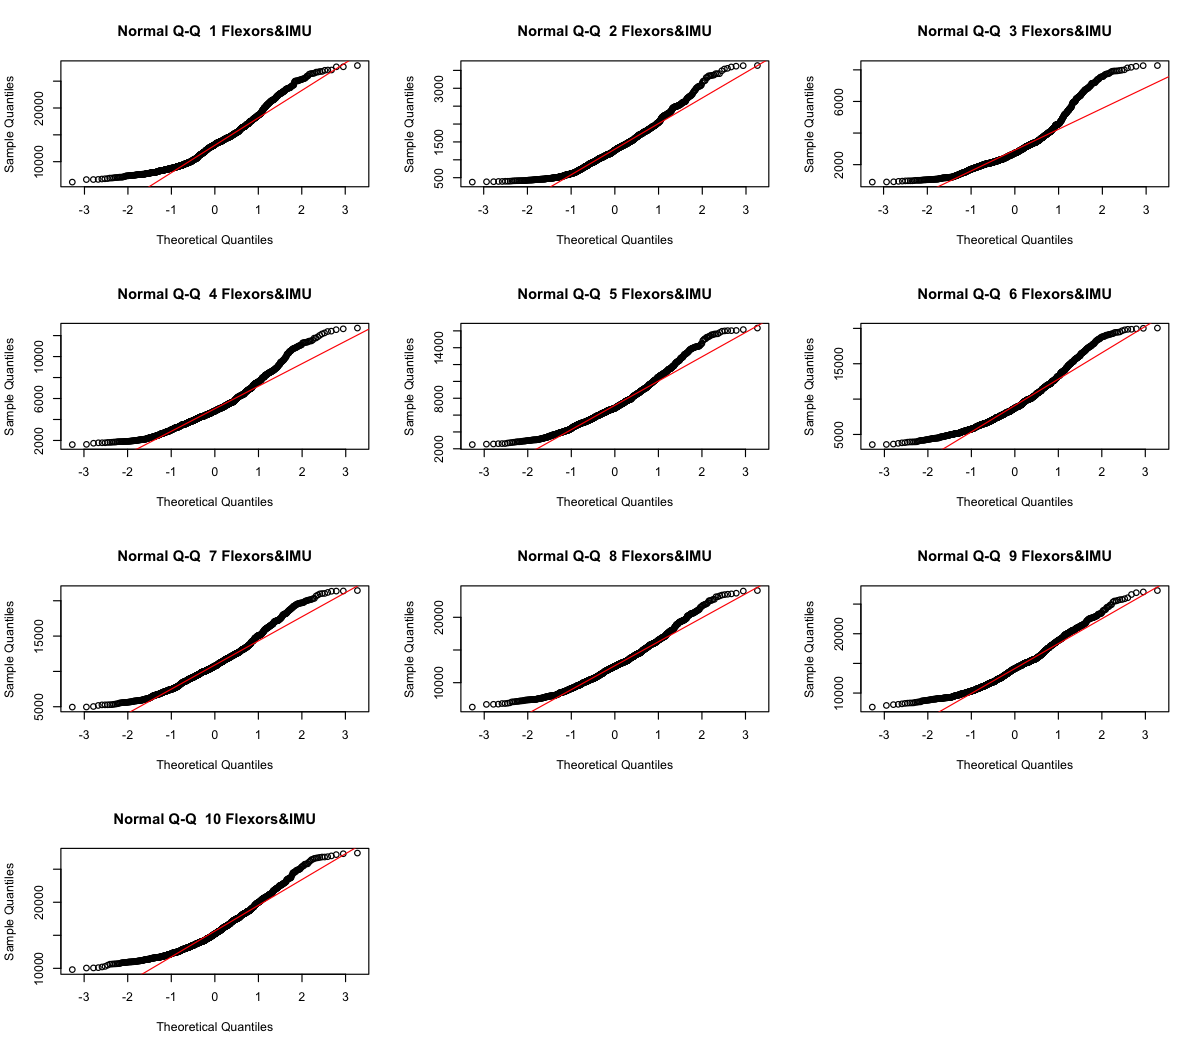
\includegraphics[width=1.0\textwidth]{evaluation/graphics/Xamarin/Galaxy-APITest/NormalQQFlexors&IMUXamarinGalaxy-APITest.png} 
   	\centering
    \caption[Gráfico QQ de Flexores e IMU usando API C\# ]{Flexores e IMU usando API C\# \\Fuente: elaboración propia (2018)} 
    \label{fig:xamarin-galaxy-QQ-flexors&imu-api}
  \end{center}
\end{figure}

\begin{figure}[H]
  \begin{center} 
   	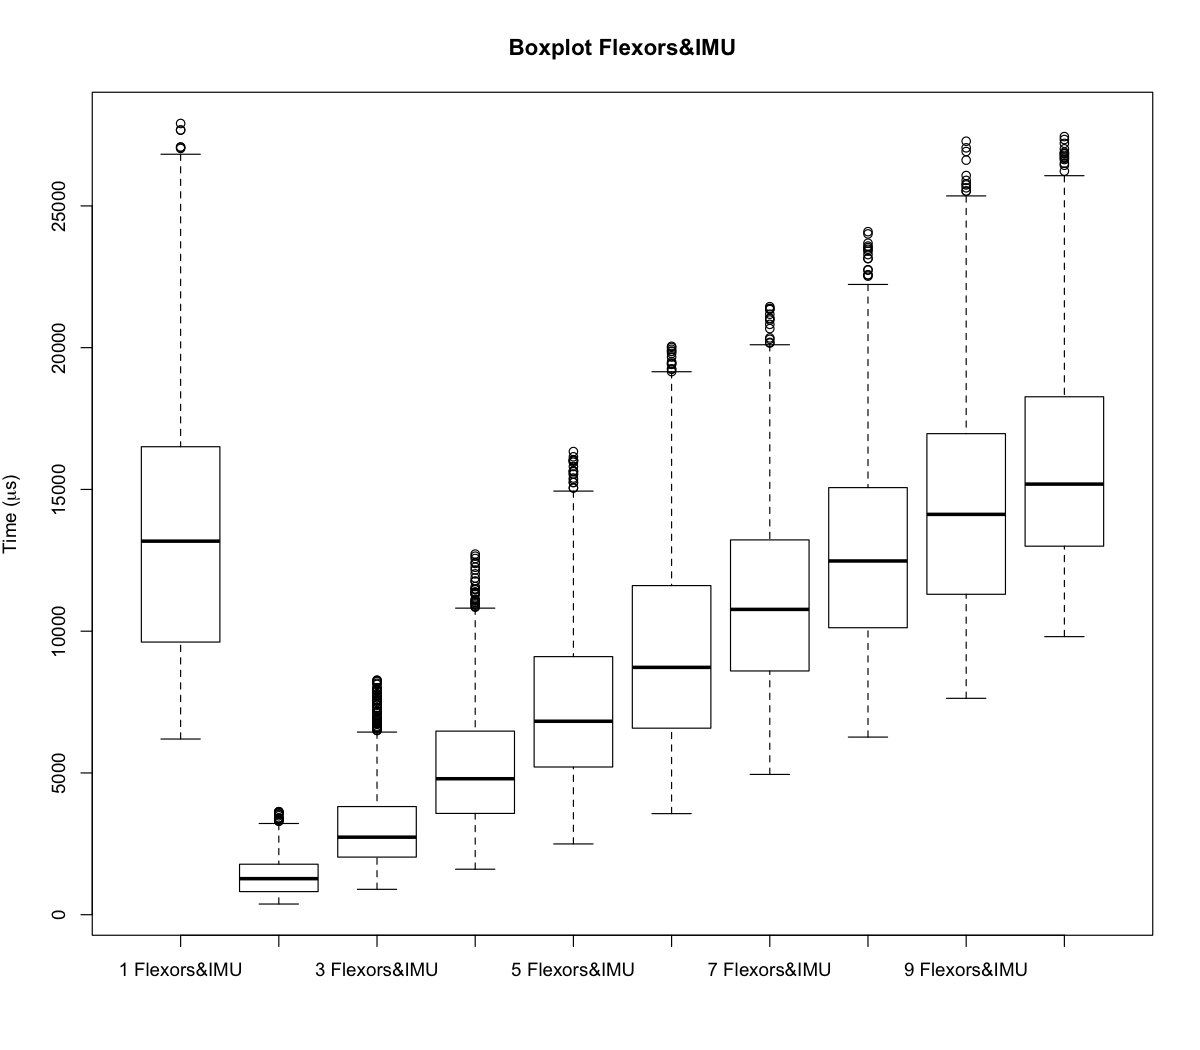
\includegraphics[width=0.8\textwidth]{evaluation/graphics/Xamarin/Galaxy-APITest/BoxplotFlexors&IMUXamarinGalaxy-APITest.png} 
   	\centering
    \caption[Gráficos de cajas de Flexores e IMU usando API C\#  ]{Gráficos de cajas de Flexores e IMU usando API C\# \\Fuente: elaboración propia (2018)} 
    \label{fig:xamarin-galaxy-boxplot-flexors&imu-api}
  \end{center}
\end{figure}

\subsection{API Java}
	\section{Resumen}
	
\newpage
\chapter{Conclusiones}
Este capítulo presenta las conclusiones del proyecto 
	\section{Objetivos}
En esta sección se concluye sobre el objetivo general y específicos del proyecto, detallando el nivel de completitud de cada uno.

\subsection{Objetivos específicos}

\subsubsection{Desarrollar la aplicación de configuración de OpenGlove en Android. Permitiendo la creación, visualización, actualización y eliminación de los perfiles de configuración:}

Se logró desarrollar la aplicación de configuración utilizando Xamarin.Forms permitiendo compartir la interfaz de usuario, realizando modificaciones mínimas según los patrones de diseño para iOS y Android. Además se logró compartir el código sobre el almacenamiento y el servidor WebSocket,  esto fue logrado utilizando paquetes de software compatibles\footnote{Paquetes de software NuGet: \url{https://www.nuget.org/packages}} con Xamarin.Forms (.NET Standar 2.0). Con esto se logró abstraer la complejidad de las configuraciones de la placa, de la IMU, los mapeos los flexores y actuadores, gracias a esta herramienta que permite configurar y administrar los distintos perfiles de configuración que pueden ser utilizados de manera independiente en cada dispositivo Bluetooth. Las diferentes iteraciones del desarrollo de esta aplicación fueron detalladas en la Sección \ref{seccion-prototipos}. La estructura y descripción puede se detalló en la Subsección \ref{subseccion-estructura-aplicacion-configuracion} de este documento.

Adicionalmente esta aplicación permite probar los actuadores, flexores e IMU previamente configurados.También permite la administración de los dispositivos Bluetooth vinculados, todo esto haciendo uso de la API C\# desarrollada en paralelo a esta aplicación.


\subsubsection{Desarrollar APIs en Java y C\# que permitan la administración de dispositivos Bluetooth en segundo plano en Android permitiendo la conexión, desconexión, activación y listado de guantes OpenGlove.  También permitirá la activación y control de actuadores, flexores e IMU} 

El desarrollo de las APIs fue realizado completamente para los dos lenguajes de programación Java y C\#, permitiendo realizar todas las funcionalidades descritas en este objetivo. Estas APIs fueron desarrolladas como clientes WebSocket que se comunican bajo un protocolo de mensajes especificado en el Anexo de este documento. Gracias a esto los desarrolladores pueden implementar diferentes funcionalidades a sus aplicaciones, como lo es el caso de la aplicación de configuración de este proyecto, el cual brinda funcionalidades que permiten probar los actuadores, flexores e IMU. La estructura y descripción de las APIs de alto nivel desarrolladas se detalla en la Subsección \ref{subseccion-estructura-apis-hl}. El comportamiento de las APIs fue detallado en la \ref{seccion-comportamiento-apis}.

%\item Implementar la autenticación mediante cuentas de Google para acceder a los perfiles de configuración en FireBase \footnote{Base de datos no relacional en la nube Firebase \url{https://firebase.google.com/?hl=es-419}}.

\subsubsection{Realizar evaluaciones de rendimiento para las APIs Java y C\# :} 
Se lograron realizar las evaluaciones de rendimiento necesarias para las APIs, considerando también las evaluaciones que buscaban comparar el desarrollo de aplicaciones nativas en Android usando Android Studio con el uso de Xamarin.Forms como herramienta multiplataforma para aplicaciones nativas. Las evaluaciones permitieron determinar los rendimientos obtenidos en los dispositivos móviles. En comparación a los resultados obtenidos en el trabajo de\cite{tesis-cerda-rodrigo}, los de este proyecto presentaron rendimientos inferiores, pero esto es debido a las limitaciones del dispositivo móvil utilizado, comparado con el ordenador en el que el trabajo previo fue evaluado. El Capítulo \ref{capitulo-evaluacion-tecnica}

\subsubsection{Demostrar el uso del SDK en un ambiente de VR, AR o MR, utilizando las APIs desarrolladas:}
Fue posible realizar una prueba de concepto simple, utilizando las herramientas de GoogleARCore/GoogleVR, generando colisiones en regiones especificadas para activar los actuadores y generando el movimiento gracias a los datos provistos por el IMU. De esta forma es posible demostrar de manera práctica el uso de las APIs en los ambientes de AR, VR o MR. la sección de pruebas 




\subsection{Objetivo general}
El objetivo general del proyecto fue desarrollar un SDK que permita dar soporte a OpenGlove en dispositivos móviles. Como producto final se obtiene una aplicación de configuración para Android, con APIs en lenguajes de programación Java y C\#. Se proporciona un SDK para dispositivos móviles de Código Abierto (Open Source) que incluye las APIs de alto nivel, la documentación y todo los recursos generados durante el desarrollo del proyecto (prototipos, iconos, imágenes, diagramas, etc.) 
	\section{Resultados obtenidos}
Esta sección se concluye sobre los resultados obtenidos sobre el desarrollo de software y los resultados de las pruebas realizadas en el presente trabajo.

\subsection{Desarrollo de software}
El desarrollo de software de este proyecto tiene como producto final el SDK para dispositivos móviles, el cual se compone de las APIs de alto nivel, la aplicación de configuración, pruebas de concepto y toda la documentación generada durante el proyecto. Estas APIs desarrolladas en Java y C\# dan soporte a la gestión de dispositivos Bluetooth, los actuadores, sensores de flexibilidad  y sensor de rastreo IMU. Pudiendo hacer uso de estas en ambientes de Realidad Virtual, Aumentada o Mixta en dispositivos móviles, con tecnologías que sean compatibles con los lenguajes de programación ya mencionados.

\subsection{Resultados de las pruebas}
	
	Los resultados de las pruebas de rendimiento son aceptables dado que no superan el umbral de latencia máximo que las personas pueden detectar. Esto puede ser mejorado utilizando dispositivos con mayores prestaciones que el utilizado en las pruebas de rendimiento, por tanto, las especificaciones de Hardware del dispositivo móvil utilizado, se plantean como requerimientos mínimos recomendados para utilizar OpenGlove en Android, considerando siempre disponer de prestaciones superiores de acuerdo a los requerimientos mínimos para las aplicaciones de Realidad Virtual, Aumentada o Mixta.
%	\subsubsection{Tiempo de respuesta}
%	\subsubsection{Líneas de código}
	\section{Alcances y limitaciones}
	\section{Trabajo futuro}

\begin{itemize}
	\item Redactando ...
	\item Dar soporte del SDK en iOS, desarrollando los componentes específicos faltantes.
	\item Desarrollar patrones de activación de actuadores extensibles en las APIs de alto nivel, para evitar que el desarrollador deba crear sus propios patrones básicos cada vez, y que pueda extender estos patrones.
	\item Extender el protocolo de comunicación de las APIs de alto nivel al SDK de Windows, para soportar la activación de actuadores mediante mensajes utilizando WebSocket.
	\item Ver la posibilidad de extender este proyecto en otras plataformas\footnote{Plataformas soportadas por Xamarin.Forms \url{https://github.com/xamarin/Xamarin.Forms/wiki/Platform-Support}}, dado que Xamarin.Forms Android, iOS y UWP (universal Windows Platform) en una versión estable.
\end{itemize}
	\section{Observaciones finales}

{\setstretch{1.0}						% Interlineado en las páginas finales
% ### Optativo: Glosario ###
\clearpage
\addcontentsline{toc}{chapter}{Glosario}
\glosario{

\begin{itemize}

\item \textbf{Actuadores:} Un actuador es un dispositivo inherentemente mecánico cuya función es proporcionar fuerza para mover o ``actuar” otro dispositivo mecánico. La fuerza que provoca el actuador proviene de tres fuentes posibles: Presión neumática, presión hidráulica, y fuerza motriz
eléctrica (motor eléctrico o solenoide). Dependiendo de el origen de la fuerza el actuador
se denomina ``neumático'',  ``hidráulico'' o ``eléctrico''  \citep{actuadores}. 

\item \textbf{API:} \textit{Application Program Interface} por sus siglas en inglés es código que actúa como interfaz para la programación de aplicaciones, permitiendo por ejemplo, que dos aplicaciones se comuniquen entre si, como el acceder a funcionalidades sin la necesidad de conocer la complejidad del código implementado\citep{techtarget-API}.

\item \textbf{Augmented Reality (AR):} La realidad aumentada (AR) es el uso de información en tiempo real en forma de texto, gráficos, audio y otras mejoras virtuales integradas con objetos del mundo real. Es este elemento del ``mundo real'' lo que diferencia a AR de la realidad virtual. AR integra y agrega valor a la interacción del usuario con el mundo real, frente a una simulación. \citep{gartner-group-AR}.

\item \textbf{Haptic Feedback:} Haptics es una tecnología táctil o de retroalimentación de fuerza que aprovecha el sentido del tacto de una persona al aplicar vibraciones y / o movimiento a la punta del dedo del usuario. Esta estimulación puede ayudar a la tecnología en el desarrollo de objetos virtuales en la pantalla del dispositivo. En su sentido más amplio, hápticos puede ser cualquier sistema que incorpore elementos táctiles y vibre a través de un sentido del tacto \citep{gartner-group-haptics}.

\item \textbf{IMU (Inertial Measurement Unit):} Los sensores inerciales, también llamados IMU (Unidad de medición inercial), son dispositivos electrónicos de medición que permiten estimar la orientación de un cuerpo de las fuerzas inerciales que el cuerpo experimenta. Su principio de funcionamiento se basa en la medición de las fuerzas de aceleración y velocidad angular ejercidas independientemente en masas pequeñas ubicadas en el interior \citep{IMU-sensor-01}.

\item  \textbf{OpenGlove:} es un guante desarrollado por la Universidad de Santiago de Chile, por el grupo de investigación y desarrollo Interaction, el cual provee \textit{haptic feedback} o retroalimentación táctil en ambientes virtuales, como también la captura de movimientos de la mano \citep{openglove-info-page}.

\item \textbf{Mixed reality (MR):}  La realidad mixta es el resultado de mezclar el mundo físico con el mundo digital. La realidad mixta es la siguiente evolución en la interacción entre el hombre, la computadora y el entorno, y abre posibilidades que antes estaban restringidas a nuestra imaginación. Es posible gracias a los avances en visión artificial, potencia de procesamiento gráfico, tecnología de visualización y sistemas de entrada. El término realidad mixta fue presentado originalmente en un artículo de 1994 por Paul Milgram y Fumio Kishino, ``Una taxonomía de visualizaciones de realidad mixta". Su trabajo introdujo el concepto del continuum de virtualidad y se centró en cómo se aplica la categorización de la taxonomía a las exhibiciones. Desde entonces, la aplicación de la realidad mixta va más allá de las pantallas, pero también incluye la información ambiental, el sonido espacial y la ubicación. \citep{microsoft-MR}.

\item \textbf{SDK:} conjunto de utilidades de desarrollo para escribir aplicaciones de software, generalmente asociadas a entornos específicos (por ejemplo, el SDK de Windows) \citep{gartner-group-SDK}.

\item \textbf{UX:}	La ``experiencia de usuario'' abarca todos los aspectos de la interacción del usuario final con la empresa, sus servicios y sus productos \citep{nngroup-ux}.

\item \textbf{Virtual Reality (VR):}  La realidad virtual (VR) proporciona un entorno 3D generado por computadora que rodea al usuario y responde a las acciones de esa persona de forma natural, generalmente a través de pantallas inmersivas montadas en la cabeza y el seguimiento de la cabeza. También se pueden usar guantes que proporcionen seguimiento de las manos y retroalimentación háptica (sensible al tacto). Los sistemas basados en sala brindan una experiencia 3D para múltiples participantes; sin embargo, son más limitados en sus capacidades de interacción. \citep{gartner-group-VR}.

\item \textbf{WebSocket}: WebSocket es un protocolo que provee un canal de comunicación bidireccional y simultáneo (full-duplex) entre un cliente y un servidor, utilizando un único socket TCP (Transmission Control Protocol). \citep{websocket-html5}

\end{itemize}

}

% ### Bibliografía de la tesis ###
\clearpage
\addcontentsline{toc}{chapter}{Referencias bibliogr\'aficas} % Comando para agregar el índice a la Tabla de
\bibliographystyle{apa-good}
\bibliography{bibliografia}

% ### Optativo: Anexos de la tesis ###
%\clearpage
%\anexo
%\addcontentsline{toc}{chapter}{Anexos}

%\chapter{Título del anexo ejemplo}
\label{finales:anexo1}
El 15 de junio del 2012 la Agencia Acreditadora Colegio de Ingenieros de Chile S.A., otorga la acreditación de la carrera de Ingeniería Civil Informática de la Universidad de Santiago de Chile sede Santiago, en sus jornadas diurna y vespertinas por un plazo de 5 años.
% ### Anexos ###

% ### Optativo: Apéndices de la tesis ###
%\clearpage
%\apendice
%\addcontentsline{toc}{chapter}{Apéndices}

% ### Apéndices ###
%\chapter{Título del apéndice ejemplo}
\label{finales:apendice1}
El 15 de junio del 2012 la Agencia Acreditadora Colegio de Ingenieros de Chile S.A., otorga la acreditación de la carrera de Ingeniería Civil Informática de la Universidad de Santiago de Chile sede Santiago, en sus jornadas diurna y vespertinas por un plazo de 5 años.
} % end \setstretch{1.0}

\end{document}
% end